\documentclass[
draft,
oneside,
% paper=B5,
% openright,
% DIV=13,
% BCOR=5mm,
]{scrbook}

\usepackage{mathtools}
\usepackage[final]{pdfpages}
\usepackage{amsfonts}
\usepackage{biblatex}
\usepackage{xcolor}
\usepackage{graphicx}
\usepackage{bm}
\usepackage{braket}
\usepackage{amsthm}
\usepackage{microtype}
\usepackage{thmtools}
\usepackage{siunitx}
\usepackage{subcaption}
\usepackage{tikz}
\usepackage{pgfplots}
\usepackage{pgfplotstable}
\usepackage{hyperref}
\usepackage{float}
\usepackage{etoolbox}
\usepackage{booktabs}
\usepackage{multirow}
\usepackage[final]{listings}
\usepackage{cleveref}
\usepackage{comment}
\usepackage{slashed}  % Gives the /slashed{A} macro. Consider in the future to switch with manually greated macro /slashed made from /not operator, as read in forum (supposedly looks better)
\usepackage[acronym]{glossaries}
\usepackage{hyperref}
\hypersetup{
hidelinks,
final=true,
}
\usepgfplotslibrary{colormaps}
\pgfplotsset{compat=1.18}
\usepgfplotslibrary{groupplots}
\usepgfplotslibrary{external}
\tikzexternalize
\tikzsetexternalprefix{figures/external/}
% \pgfkeys{/pgf/images/include external/.code={\href{file:#1}{\pgfimage{#1}}}} %% for draft mode. See pgf manual
\pgfkeys{/pgf/images/include external/.code={\href{file:#1}{\includegraphics[draft=false]{#1}}}} %% for draft mode. See pgf manual

\setacronymstyle{short-long}

\addbibresource{Master.bib}
\addbibresource{manual.bib}
\renewcommand\multicitedelim{\addsemicolon\space}


% \usepackage{fancyhdr}

%%% Header %%%%
% Layout 0
% \pagestyle{fancy}
% \addtolength{\headwidth}{\marginparsep}
% \addtolength{\headwidth}{\marginparwidth}
% \renewcommand{\chaptermark}[1]{\markboth{#1}{}}
% \renewcommand{\sectionmark}[1]{\markright{\thesection\ #1}}
% \fancyhf{}
% \fancyhead[LE,RO]{\textbf{\thepage}}
% \fancyhead[LO]{\textbf{\rightmark}}
% \fancyhead[RE]{\textbf{\leftmark}}
% \fancypagestyle{plain}{%
% \fancyhead{} % get rid of headers
% \renewcommand{\headrulewidth}{0pt} % and the line
% }
% Layout 1
% \pagestyle{fancy}
% % \addtolength{\headwidth}{\marginparsep}
% \addtolength{\headwidth}{\marginparwidth}
% \renewcommand{\chaptermark}[1]{\markboth{\MakeUppercase{#1}}{}}
% \renewcommand{\sectionmark}[1]{\markright{\thesection.\ #1}}
% % \fancyhead[LE,RO]{\thepage}
% \fancyhead{}
% \fancyhead[RO]{\rightmark}
% \fancyhead[LE]{\leftmark}
% \fancyfoot{}
% \fancyfoot[LE,RO]{\thepage}

% % Layout 2 %%
% \pagestyle{fancy}
% \renewcommand{\chaptermark}[1]%
% {\markboth{\MakeUppercase{\thechapter.\ #1}}{}}
% \renewcommand{\sectionmark}[1]%
% {\markright{\MakeUppercase{\thesection.\ #1}}}
% \renewcommand{\headrulewidth}{0.5pt}
% \renewcommand{\footrulewidth}{0pt}
% \newcommand{\helv}{%
% \fontfamily{phv}\fontseries{b}\fontsize{9}{11}\selectfont}
% \fancyhf{}
% \fancyhead[LE,RO]{\helv \thepage}
% \fancyhead[LO]{\helv \rightmark}
% \fancyhead[RE]{\helv \leftmark}

\newcommand{\cbox}[2][yellow]{%
  \colorbox{#1}{\parbox{\dimexpr\linewidth-2\fboxsep}{\strut #2\strut}}%
}
\newcommand{\todo}[2][orange]{\hfill\break{\bfseries\cbox[#1]{#2}}\break}
% \renewcommand{\todo}{\empty}

% \setlength\multlinegap{0pt}  %% Make multline go all the way left

\newcommand{\pe}{\phantom{=}}
% \newcommand{\sign}{\operatorname{sign}}
\DeclareMathOperator\sign{sign}
\DeclareMathOperator\arctanh{arctanh}
\renewcommand{\vec}{\bm}
\renewcommand{\Im}{Im}
\DeclareMathOperator{\Tr}{Tr}
\newcommand{\qvec}[1]{\mathfrak{#1}} % Used for two-dim vec

\declaretheorem[thmbox=S]{Proposition}
\declaretheorem[thmbox=M, style=remark]{summary}
\declaretheoremstyle[
    spaceabove=6pt,
    spacebelow=6pt,
    headfont=\normalfont\itshape,
    bodyfont = \normalfont,
    postheadspace=1em,
    qed=\( \square \),
    headpunct={:}]{myproofstyle}
\declaretheorem[style=myproofstyle, unnumbered]{Proof}
\declaretheorem[name=Theorem]{theorem}

% \newcommand{\gls}[1]{#1}  % Hack until glossaries work
\newacronym{qed}{QED}{quantum electrodynamics}
\newacronym{qft}{QFT}{quantum field theory}
\newacronym{trim}{TRIM}{time reversal independent momenta}
\makeglossaries


\begin{document}
% \includepdf{frontpagethesis.pdf}
\frontmatter
\tableofcontents

\mainmatter
\chapter{Topological materials}
\section[Weyl and Dirac cones]{Weyl and Dirac cones in condensed matter physics}
\label{sec:weyl-dirac-cones}
%% Much is taken from https://www.tandfonline.com/doi/pdf/10.1080/00018732.2014.927109?needAccess=true
Dirac and Weyl cones are the emergence of non-gapped linear energy bands in condensed matter physics, in effect exhibiting relativistic behavior at non-relativistic speeds.
We here give a very brief introduction to these materials.
Firstly, we will consider the so-called band crossing, and how the opening of a gap at the band crossing behaves differently in two and three dimensions.
Then, various perturbations that do not open a gap will be considered, giving interesting effects in the dispersion relations.
Lastly, a consideration of these materials in light of Berry curvature and the topological quantity of Chern numbers will be given.

While the nearly free quasi-particle model performs very well for most metals, with the Hamiltonian $p^2 / (2m^*)$, with $m^{*}$ some effective mass, this model fails for the Dirac-materials.
Instead of obeying the Schrödinger equation as most materials, they obey a Dirac equation, with the speed of light being replaced by the Fermi velocity $v_F$.
As in the high energy case, the Dirac equation may be decomposed into chiral Weyl equations in the massless case.
Setting $v_F = 1$ for simplicity one gets the Hamiltonian
\begin{equation}
  \label{eq:27}
H_D = s v_{F} \vec{\sigma} \vec{p},
\end{equation}
where $\vec{\sigma}$ are the Pauli matricies, $v_F$ the Fermi velocity, $\vec{p}$ the momentum, and $s=\pm 1$ denotes the chirality.
% It is here important to note that the spin degree of freedom expressed by the Pauli matricies, may either be real spin or some pseudo spin degree of freedom.
It is here important to note that the Pauli matrices represent either real spin degree of freedom or some pseudo spin degree of freedom.
Examples of pseudo spin is that of bipartite lattices, such as Graphene, in which case one must be careful when for example applying time reversal, as only real spin is odd under this operation, and not pseudo spin.

The dispersion of the Hamiltonian (\ref{eq:27}) has a band crossing at  $\vec{p} = 0$.
For the two-dimensional case, a perturbation on the form $m \sigma_z$, with $m$ some parameter, can open up a gap in the dispersion relation.
This is easily verified by writing out the Hamiltonian and solving the eigenproblem
\begin{align}
  H_D^{(2D)} &= s v_{F} (p_x \sigma_x + p_y \sigma_y) + m \sigma_z.\\
  \left|
  H_D^{(2D)} - E
  \right| &= 0.
\end{align}
As the Hamiltonian commutes with the momentum operator, we replace the momentum operator with its eigenvalues
\begin{equation}
E = \pm v_F \hbar \sqrt{k_x^2 + k_y^2 + \frac{m^2}{\hbar ^2 v_{F}^2}}.
\end{equation}
There are no solutions $k_x, k_y$ making the energy levels degenerate.
The crossing is thus only protected by symmetry considerations, and is not \emph{topologically protected}.

In three dimensions the situation is somewhat different, with the Hamiltonian  
\begin{equation}
  H_D^{(3D)} = s v_F ( p_x \sigma_x + p_y \sigma_y + p_z \sigma_z).
\end{equation}
In this case, no perturbing term may open a gap at the crossing.
There is no $2\times 2$ matrix $\sigma_4$ that anticommutes with the Pauli matricies and also is linearly independent, i.e. there is no ``fourth'' Pauli matrix, and thus no perturbative term will open the gap.
Say for example we add a term like $m \sigma_z$, where the $z$-direction was chosen arbitrarily.
The only effect this will have on the crossing is to translate it in $p_z$.
Tying this back to the accidental degeneracy, we see that no matter the perturbation, the three-dimensional momentum space will always have a point of degeneracy, i.e., a crossing.
The crossing is \emph{topologically protected}.
A more formal approach to topological materials, is that of topological invariants -- numbers related to the topology of the material.
Having a non-trivial topological invariant number, is the very definition of topological materials, and we will in subsection \ref{sec:chern-number-weyl} show that Dirac cones makes the Chern number of these materials non-trivial.

The Hamiltonian in Eq. (\ref{eq:27}) is not the most general, if we allow for anisotropy in the system.
In three dimensions we have more generally the Hamiltonian
\begin{equation}
  \label{eq:38}
  H(\vec{k}) = \vec{v}_0 \vec{k} + (\vec{v} \odot \vec{k}) \vec{\sigma} ,
\end{equation}
where $\vec{v}_0$ is  the \emph{tilt vector}, $\vec{v}$ is some, anisotropic velocity, $(\vec{v} \odot \vec{k})_i = v_i k_i$ is the Hadamard product of the anisotropic velocity and the momentum,  and $\vec{\sigma}$ are the Pauli matrices corresponding to spin degree of freedom.
Here we will consider two interesting cases.
Firstly, we will consider perturbations in the tilt-less isotropic case, $\vec{v}_0 = 0,  \vec{v}_i = v_F \hat{x}_i$.
Then, a tilted system without perturbations is considered.

Consider an isotropic tilt-less system;
introduce to the system a pseudospin degree of freedom, thus extending the system to $4\times 4$-matricies.
The Hamiltonian of the system~\cite{armitageWeylDiracSemimetals2018a}
\begin{equation}
  \label{eq:29}
  H = v_F \tau _x \otimes \vec{\sigma} \vec{k} + m \tau _z \otimes I_2 + b I_2 \otimes \sigma _z + b' \tau _z \otimes \sigma _x,
\end{equation}
with $\vec{\tau}$ the Pauli matricies related to the pseudospin, and $I_2$ the identity matrix of dimension 2.
The perturbing parameters $m, b, b'$ are a mass parameter, and Zeeman fields in the $z$ and $x$ direction, respectively.
Ignore for now $b'$, i.e. $b' = 0$, which is related to a state known as the line node semimetal.
Notice  that the $b$ term breaks time reversal symmetry in the system, as the real spin $\sigma $ is odd under time reversal.
The eigenvalues of this system~\cite{armitageWeylDiracSemimetals2018a}
\begin{equation}
  E_{s \mu }(\vec{k}) = s \left[
    m^2 + b^2 + v_{F}^2k^2 + 2 \mu  b \sqrt{v_F^2 k_z^2 + m^2}
  \right]^{\frac{1}{2}},
\end{equation}
with $s=\pm 1, \mu = \pm 1$ encoding the degeneracies related to the spin and pseudospin degrees of freedom, respectively.
There are still linear dispersions for $b > m$.
For $b < m$, a gap opens, and the dispersion is non-linear.
In fact, this is simply a shift in $k_z$ of the Dirac cone, as  is seen by rewriting
\begin{equation}
  E_{s \mu }(\vec{k}) = s v_F
  \left[
    k_x^2 + k_y^2 + \left( \sqrt{k_z^2 +  \frac{m^2}{v_{F}^2}} + \mu \frac{b}{v_{F}} \right)^2
  \right]^{\frac{1}{2}}.
\end{equation}
This still has Weyl node solutions at $k_z^2 = (b^2-m^2) /v_F^2$, where the dispersion is linear in the vicinity of the nodal solutions.
This thus separates two Dirac nodes in momentum space, giving  a \emph{Weyl} semimetal.
This also illustrates that the decomposition in Eq. (\ref{eq:27}) is valid around either of the shifted nodes.
Expanding around one of the Dirac points of the Weyl semimetal, the Hamiltonian is exactly Eq. (\ref{eq:27}), after decomposing the $4 \times 4$ Hamiltonian into its two chiral  $2\times 2$ Weyl constituents.

If one instead perturbs the system with a Zeeman field in the $x$-direction, i.e. having a $b' > 0$, the splitting is instead in energy, giving nodal loop where the two cones intersect.
We will not go into any depth on these types of materials.
\todo{Possibly rewrite the following sentence}
The three cases described here: unperturbed, where the two cones are superimposed; perturbed by $b$, where the cones are separated in momentum; and perturbed by $b'$, where the cones are separated in energy, are shown in Figure \ref{fig:conetypes}.
Notice that in the two latter cases, the Dirac points, i.e. crossings, are not superimposed.
As will be discussed in section \ref{sec:weyl-dirac-cones}, this makes the crossings very robust, as the two nodes must merge before a gap may be opened.

The second case to consider, is a finite tilting vector $\vec{v}_0$, where we will consider only real spin, thus reducing the system back to the two-dimensional case in Eq. (\ref{eq:38}).
For the isotropic case, $\vec{v}_i = v_F \hat{x}_i$, the energy bands are~\cite{ottesenOpticalConductivityDirac2021}
\begin{equation}
  E_s(\vec{k}) = \vec{v}_0 \vec{k} + s v_F |k|.
\end{equation}
Tehse types of systems, which are the systems of interest for this thesis, are considered in detail in section \ref{sec:typeii}.

\begin{figure}[p!]
  \centering
  % \includegraphics[width=\textwidth]{figures/cone}
  % \includegraphics[width=\textwidth]{figures/cones_types-verysmall}
  \includegraphics[width=\textwidth]{figures/cones-types-col1-opaque.png}
  \caption{Dispersion curves in the $k_z, k_x$-plane. \textbf{(Left)} Dirac material with superimposed cones. \textbf{(Center)} Time reversal symmetry broken, giving a Weyl material with the cones separated in momentum  space. \textbf{(Right)} The cones shifted in energy, givng a nodal loop.}
  \label{fig:conetypes}
\end{figure}

\begin{figure}[p!]
  \centering
  % \includegraphics[width=0.75\textwidth]{figures/tilt_cone}
  % \includegraphics[width=0.75\textwidth]{figures/conesTransparent-verysmall.png}
  \includegraphics[width=\textwidth]{figures/cones-tilt-color1.png}
  \caption{Tilted Dirac cones.
    From left to right the tilt increases, from no tilt in the first cone to overtilt in the last.
    The three first are Type-I Weyl semimetals, the last is a Type-II semimetal.
    See main text for details.
  }
  % \caption{Tilted cone. \textbf{(Left)} Type I Weyl semimetal, with no tilt.
  %   \textbf{(Center)} Type  I Weyl semimetal, with tilt.
  %   \textbf{(Right)} Type II Weyl semimetal, meaning the tilt makes the upper part of the cone go below horizontal.}
  \label{fig:tiltcone}
\end{figure}

\subsection{Chern number of the Weyl point}\label{sec:chern-number-weyl}
In order to more explicitly demonstrate the topological nature of the state in Eq. (\ref{eq:27}), we will find a non-zero topological invariant associated with that state.
Thereby showing that the material is a topological material.
The topological number we will calculate is the Chern number, related to the Berry curvature of the bands in some enclosed surface.
In order to calculate the Chern number, we must first find an expression for the Berry curvature of our system.
This derivation will follow closely Berry's original derivation~\cite{berryQuantalPhaseFactors1984} of the Berry phase of a two-level system with the Hamiltonian
\begin{equation}
  \label{eq:30}
  H(\vec{R}) = \frac12 \vec\sigma \vec{R}.
\end{equation}
Some notation has been modernized with inspiration from the treatment of the Berry phase of the spin-$1 /2$ particle in an external magnetic field in~\citeauthor{holsteinAdiabaticTheoremBerry1989}~\cite{holsteinAdiabaticTheoremBerry1989}.

Suppose we have a Hamiltonian $H(t)$, and that its $t$-dependence can be parameterized by $\vec{R} = \vec{R}(t)$, as in $H(t) = H(\vec{R}(t))$.
Any evolution of the Hamiltonian through time, may then be described as a geometric path through the $\vec{R}$-space.
As the reader might be aware, Berry's most famous discovery was that a closed path through $\vec{R}$-space gives an observable phase to the system, unlike the non-physical dynamical phase, which may be removed by a suitable choice of gauge.
Here we will however focus on the so-called Berry curvature, $\vec{B}$, a vector field which will be shown to be useful in the categorization of topological materials.
Note that there is some variation in the literature on the naming of the various quantities, and the sign convention used.
In particular, the word Berry curvature will in some literature refer to a rank two tensor, while our quantity $\vec{B}$ is referred to as the Berry field strength.
In particular, if we let the rank two tensor be denoted $F_{ij}$, the Berry field strength $\vec{B}$ is given by
\begin{equation}
  B_i = \epsilon_{ijk} F_{jk}.
\end{equation}
\todo{Consider rewriting some of  this. Look in topology book}
The Berry curvature for the state $n$ is explicitly defined as~\cite{berryQuantalPhaseFactors1984}
\todo{Should we add some more comments about adabiatic? See topo book}
\begin{equation}
  \vec{B_n}(\vec{R}) =
  -\Im \sum_{m\neq n}
  \frac{
    \braket{n(\vec{R}) | \nabla_{\vec{R}} H | m(\vec{R}) }
    \times
    \braket{m(\vec{R}) | \nabla_{\vec{R}} H | n(\vec{R}) }
  }{
    (E_m(\vec{R}) - E_n(\vec{R}))^2
  },
\end{equation}
where $\times $ denotes the cross product.
Notice that for a degeneracy $E_n = E_m$ there will be an infinity in $\vec{B_n}$.
Considering the Berry curvature as a field in $\vec{R}$-space, this resembles a source, as will become relevant later.
This may now be applied to for example the Weyl semimetal, both in the interest of solidifying the above theory, and as it will be useful in future  consideration.

The Hamiltonian around the Weyl point is
\begin{equation}
  H = v_F \vec\sigma \cdot \vec{p},
\end{equation}
with $v_F$ the Fermi velocity, $\vec{\sigma}$ the Pauli matrices, and $\vec{p}$ the momentum operator.
% \todo{Now suddenly R is not dependent  on t??}
By letting $\vec{R} = v_F \vec{p}$, the Berry curvature of the Hamiltonian can be found.
The eigenvalues of this system are
\begin{equation}
    E_+ = -E_-
    = |R|.
\end{equation}
The aforementioned degeneracy is here of course the Weyl point, where $E_+ = E_- = 0$.
Noting that
\begin{equation}
  \nabla_{\vec{R}} H = \vec\sigma,
\end{equation}
we can calculate the Berry curvature easily.
Denote by $\ket{+}$ the state with the eigenvalue $E_+$ and $\ket{-}$ the state with the eigenvalue $E_-$.
Take also, without loss of generality, $\vec{R}$ to be in the $z$-direction.
This gives
\begin{equation}
  \vec{B}_+ = -\Im
  \frac{
    \braket{+ | \vec\sigma | -}
    \times
    \braket{- | \vec\sigma | +}
  }{
    4 R^2
  }.
\end{equation}
As $\ket{+}$ and $\ket{-}$ are eigenstates of $\sigma_z$ and orthogonal to each other, only the $z$-component of the cross product may contain non-zero contributions.
\begin{equation}
  \begin{split}
    \vec{B}_+ &= - \frac{\hat{z}}{4 R^2}
    \Im \left(
    \braket{+ | \sigma_x | -}
    \braket{- | \sigma_y | +}
    -
    \braket{+ | \sigma_y | -}
    \braket{- | \sigma_x | +}
    \right)\\
    &= - \frac{ \hat{z}}{2 \vec{R}^2}.
  \end{split}
\end{equation}
Here, the effect of the Pauli matrices on the eigenvectors was used, according to
\begin{align}
  \sigma_x \ket{\pm} &= \ket{\mp}\\
  \sigma_y \ket{\pm} &= \pm i \ket{\mp}
\end{align}
Returning to general axis orientations, one has
\begin{equation}
  B_+ = - \hat{R} / 2\vec{R}^2 = - \vec{R} / 2 \vec{R}^3.
\end{equation}
For the $\ket{+}$-band, the Weyl point thus takes the form of a negative monopole in $R$-space;
this motivates the requirement that Weyl points must always appear in pairs of opposite chirality, as the divergence of the Berry curvature must always be zero over the entire sample.
\todo{There should probably be some care taken here with the sign of $v_F$.}

As mentioned, the Chern number is one of several numbers that is used to classify topological materials.
The Chern number is defined as
\begin{equation}
  C = \frac{1}{2\pi} \oint_{\partial C} \vec{B_+} \cdot \mathrm{d}\vec{S},
\end{equation}
where the integral is taken over the closed surface $\partial C$, enclosing the volume $C$.
Noting that the Berry curvature has the shape of a monopole source at $\vec{p} = 0$, we immediately know the value of this quantity from electromagnetism.
We will, however, carry out the computation explicitly here.
With the divergence theorem in mind, it behooves us to find the divergence of the Berry curvature.
This divergence is zero everywhere except in the monopole source, giving
\begin{equation}
  \nabla \cdot \vec{B_+} = -\frac12 \nabla \cdot \hat{R} / R^2 = -2 \pi \delta(\vec{p}),
\end{equation}
where $\delta$ is the Dirac delta distribution.
By virtue of the divergence theorem the Chern number is then found to be
\begin{equation}\label{eq:chern}
  C = \frac{1}{2\pi} \int_C \nabla \cdot \vec{B_+} \mathrm{d} C = -1,
\end{equation}
where the property of integrals over Dirac delta distributions was used.

Note that some literature will have a Chern number differing from \eqref{eq:chern} by the sign of the Fermi velocity,
\begin{equation}
  C = - \operatorname{sign}(v_F).
\end{equation}
This simply comes from the definition of the eigenstates.
We have put the sign dependence in the state, making the $E_+$ state always have positive eigenenergy.
In literature that instead defines $E_+ = v_F |R|$ the state's energy will depend on the sign of the Fermi velocity, and as a consequence, the sign dependence will end up in the Chern number instead.

The overall divergence of Berry curvature must be zero, or equivalently, the sum of the Chern numbers must be zero.
The Hamiltonian Eq. (\ref{eq:30}) chosen with the opposite chirality,
\begin{equation}
  H(\vec{R}) = -\frac{1}{2} \vec{\sigma} \vec{R},
\end{equation}
has the opposite Berry curvature, and also the opposite Chern number.
Thus, Dirac cones must appear in pairs of opposite chirality, either superimposed as the Dirac semimetal case or separated in momentum space, as the Weyl semimetal.
\todo{Make sure there is no discrepancy between 2D/3D materials above}

In light of the interpretation of the Dirac point as a monopole of Berry curvature, the discussion at the beginning of section \ref{sec:weyl-dirac-cones} on the stability of the band crossing in two and three dimensions gets an intuitive and geometric interpretation.
In Figure~\ref{fig:curvature_plane} the Berry curvature pole is shown in $p$-space, together with a plane parallel to the $xy$-plane, which we will denote the \emph{state plane}.
In the two-dimensional case, the state is confined to the state plane, with the $z$-position of the plane given by any mass terms $m \sigma _z$.
In the three-dimensional case, the state not confined to this plane, as the parameter $p_z$ is a free variable, or alternatively it may be considered as a freedom to move the state plane freely, with its initial position simply shifted by any mass terms.
It is thus obvious that one may never reach the monopole in the two-dimensional case, and thus for no $\vec{k}$ is there a band crossing.
Importantly, the Berry curvature is indeed non-zero, however any closed  curve of integration will give a Chern number of zero;
the  monopole has been moved outside the dimensionality of freedom.
\begin{figure}[ht]
  \centering
  \includegraphics[width=0.5\textwidth]{figures/berryCurvePlanewpath.png}
  \caption{The state plane, transparent yellow, parallel to the $xy$-plane and a Berry curvature monopole at the origin.
  An integration contour is shown in blue dashed.
  See main text for details.}
  \label{fig:curvature_plane}
\end{figure}


% \begin{figure}[ht]
%   \centering
%   \begin{tikzpicture}
%     \coordinate (O) (0,0,0);
%     \draw[->] (O) -- (5,0,0); 
%     \draw[->] (O) -- (0,5,0); 
%     \draw[->] (O) -- (0,0,5); 

%     \def\N{9}
%     \foreach \n in {0,...,\N}
%     {
%       \foreach \t in {0,...,\N}
%       {
%         \draw[->] (xyz spherical cs:radius=1.5,latitude={\n*360/\N},longitude={\t*360/\N}) -- (xyz spherical cs:radius=2,latitude={\n*360/\N},longitude={\t*360/\N});
%       }
%     }
%     \begin{scope}[canvas is zx plane at y=1.7,fill=red]
%       \draw[help lines, opacity=0.7] (-2,-2) grid (2,2);
%       \draw [cyan,thick] plot [smooth cycle] coordinates { (-1,0) (1,1) (1,-2) (0,-1) (-1, -1)};
%       \node[transform shape, rotate=90, yscale=2] at (-1.7,1.5) {$z = 2$}; 
%     \end{scope}
%   \end{tikzpicture}
%   \caption{todo}
%   \label{fig:curvature_plane}
% \end{figure}

\begin{comment}
%%%%   Old text, probably to be deleted %%%%%
\newpage

While the nearly free quasi-particle model performs very well for most metals, with the Hamiltonian $\frac{p^2}{2m^*}$, this models fails for the Dirac-materials.
Instead of obeying the Schrödinger equation as most materials, they obey a Dirac equation with the speed of light being replaced by the Fermi velocity $v_F$.
$$
H_D = v_F \sigma p + m v_F^2 \sigma_z.
$$
Here the spin degree of freedom $\sigma$ is either from the actual spin of the particle or some pseudo-spin degree of freedom such as a bipartite lattice.

The origin of this form for the Hamiltonian varies for different materials.
For graphene, for example, this form of the Hamiltonian follows directly from the tight binding model with a bipartite lattice.
Notice, however, that the spin degree of freedom in this case does not come from the actual spin of the particle, but is rather a pseudo spin degree of freedom coming from the effective two level system that appears as a result of the two positions in each cell.

The band structure of the Hamiltonian is easily found.
Writing out the Hamiltonian, setting $v_F=1$ for simplicity, we get
\begin{equation}
  H_D = p_x \sigma_x + p_y\sigma_y + m \sigma_z,
\end{equation}
which has eigenvalues at
$$
| H_D - E I | = 0.
$$
This gives us the solutions
\begin{equation}
  E = \pm \sqrt{
    k_x^2 + k_y^2 + m^2
  }.
\end{equation}

Just as in the particle physics case, the Dirac equation will exhibit gapless band structures as $m\rightarrow 0$.
As introducing a term $m\sigma_z$ would break inversion symmetry, such systems cannot be gapped.
One may show that in graphene, time and inversion symmetry will force the mass term to be zero, and the gap disappears.
\end{comment}
\begin{comment}
  \begin{figure}
    \begin{tikzpicture}
      \begin{axis}[
        legend style={
          at={(0.5, 0.95)},
          anchor={north},
        },
        legend cell align=left,
        width=13cm,
        cycle list name=linestyles,
        domain=-pi/2:pi/2,
        samples=201,
        ]
        \pgfplotsset{cycle list shift=-1}
        \foreach \m in {0, 0.1, 1, 2} {
          \addplot+[forget plot] {sqrt(x^2 + \m^2)};
          \addplot+ {-sqrt(x^2 + \m^2)};
          \addlegendentryexpanded{$m=\m$}
        }
      \end{axis}
    \end{tikzpicture}
    \caption{Band structure for the 2D Weyl Hamiltonian for various values of the mass term.} 
  \end{figure}
\end{comment}

\section{Type II Weyl semimetals}

The conic section problem with the intersecting plane restricted to pass through the node of the cone is trivially seen to have two solutions: a point and two intersecting lines.
Despite this, the possibility of a Weyl cone tilted beyond the Fermi level was never considered before \citeauthor{soluyanovTypeIIWeylSemimetals2015} described this new class of Weyl semimetals in 2015.
This now seemingly obvious possibility made an already rich field even more exciting, opening up for a wider range of novel and interesting effects.
\todo{add some concrete examples or cites}

In the case of massless fermions, the particle physics equivalent of the Weyl semimetal, such a tilt is not possible, due to the requirement of Lorentz invariance \todo{add cite or explain}.
In condensed matter physics, however, this is not an issue, and it is indeed a real class of materials \todo{cite examples}.
We denote these types of materials Type-II Weyl semimetals, as opposed to Type-I.
The transition between Type-I and Type-II is abrubt -- the Fermi surface goes form a single point to two intersecting lines, in other words going from a zero dimensional to a one dimensional surface.
\todo{Make sure this is indeed a one dimensional surface. It is kind of 1DxZ(2)}
\todo{Make sure it is one dim also for the 3D case, quadric surface, not conic intersection}
Type-II also has electron and particle pockets at the Fermi level.
While the density of states for a Type-I semimetal goes to zero as one approaches the Fermi level, this causes Type-II to have a finite density of states at the Fermi level.
\todo{End with something like: all in all this gives type ii weyl semimetal manifestly different properties from tyep i, useful both in practical applications and as an interesting phenomena seen from a purely scientific perspective}

\subsection{Hamiltonian}
We will firstly consider a slightly more realistic toy model for a Weyl semimetal, with a parameter taking the system from a Type-I to a Type-II.
This is instructive both in order to more intuitively see the origin of the terms causing the tilting of the Dirac cone, and also to see how two Dirac cones in the same Brillouin zone tilt in relation to each other.
We will then continue by linearizing the model around the Weyl points, regaining the familiar form of a Dirac cone, with an additional anisotropy term causing the tilt.

Using the general time-reversal breaking model described by \citeauthor{mccormickMinimalModelsTopological2017} we have
\begin{equation}
  \begin{split}
    H(\vec{k}) &= \left[ ( \cos k_x + \cos k_z - 2 )m + 2 t (\cos k_x - \cos k_0) \right] \sigma_1\\
    &\pe - 2 t \sin k_y \sigma_2 - 2t \sin k_z \sigma_3
    + \gamma (\cos k_x - \cos k_0).
  \end{split}
\end{equation}
The model has Weyl nodes at \(\vec{K}' = (\pm k_{0}, 0,0)\), and the parameter $\gamma$ controls the tilting of the emerging cones.
A value of $\gamma=0$ gives no tilt, while for $\gamma > |2 t|$ the Type-II system emerges.
Figure \ref{fig:ridgeline} shows the cross section \(k_{y} = 0\) of the eigenvalues of this system, as \(\gamma\) is gradually increased from 0 to 0.15 \todo{verify numbers}.
The \(\gamma\)-term ``warps'' the bands, and in the limit of Type-II the hole band crosses the Fermi level into positive energy, while the particle band crosses the Fermi level into negative energies.
We call these hole and electron pockets, respectively.

Linearizing around the Weyl nodes reduces to the familiar expression of a Dirac cone
\begin{equation}
  \label{eq:1}
  H(\vec{K} ^{'\pm} + \vec{k}) \approx \mp 2 t k_{x} \sin k_{0} \sigma_{1} - 2 t (k_{y} \sigma_{2} + k_{z} \sigma_{3}) \mp \gamma k_{x} \sin k_{0} \sigma_{0}, \quad k_{x}, k_{y}, k_{z} \ll 1.
\end{equation}
When the separation between the two nodes is \(\pi\), i.e. \(k_{0} = \pi/ 2 \), the linearized Hamiltonian of around the cone, is
\begin{equation}
  \label{eq:2}
  H'(\vec{k}) = \mp 2 t k_{x} \sigma_{x} - 2t k_{y} \sigma_{y} - 2 t k_{z} \sigma_{z} \mp \gamma k_{x}.
  % h'(\vec{v}) = -2t \vec{k} \vec{\sigma} - \gamma k_{x}.
\end{equation}
However, as the two noes are brought closer together, the effective Fermi velocity in the \(x\)-direction is rescaled, and the system is anisotropic even for no tilt (\(\gamma=0\)).
The expression may be made even more clear by moving the sign \(\pm\)-sign into the tilt parameter \(\gamma\).
The Hamiltonian is invariant under a sign change of the first term, as the isotropic Dirac Hamiltonian is invariant under inversion.
In the tilt-term, we move the sign dependence into \(\gamma \), and the linearized model is
\begin{equation}
  \label{eq:3}
  H'(\vec{k}) = - 2t \vec{k} \vec{\sigma} - \gamma^{\pm} k_{x},
\end{equation}
where \(\gamma ^{\pm} = \pm \gamma \) with the upper sign corresponding to the node at \(k_{x} = + k_{0}\) and the lower sign corresponds to the node at \(k_{x} = - k_{0}\).
As expected, we get two Dirac cones, tilting in opposite direction, but with the same amount.
\todo{How does this affect the Berry curvature and chern number?}
\todo{Maybe prettier/more correct to invert ky and kz, as that would also give the opposite chirality of the dirac points}

The linearized model are accurate in describing low energy interactions around the Fermi level.
For higher energies their validity falls apart, and more complex models are warranted.
In our calculations the linear models is sufficient, and much easier to work with, and we will thus mainly consider the linear model from here on.

\begin{itemize}
  \item gives rise to cones tilting opposite direction
  \item Linearized model valid for low energy interaction. For higher energy, the perfect cone model is not valid, as the cones does in fact touch.
  \item In this model, the hole pocket is ``shared'' between the two cones. There are also models with individual pockets (see \cite{mccormickMinimalModelsTopological2017})
\end{itemize}

\begin{figure}[ht]
  \centering
  \includegraphics[width=0.4\textwidth]{figures/conicSection}
  \caption{\label{fig:conic-section-sketch} }
\end{figure}


\begin{figure}[ht]
  \centering
  \includegraphics[width=0.7\textwidth]{figures/typeIIridgeline}
  \caption{\label{fig:ridgeline} \todo{Write this} The values of the parameters were chosen to be \(m=0.15, t=-0.05, \) and \(2 k_{0}=\pi\).}
\end{figure}

\begin{figure}[ht]
  \centering
  \includegraphics[width=0.7\textwidth]{figures/movetypeiinode}
  \caption{\label{fig:typeii:move-nodes} A Type-II Weyl semimetal with separation between the nodes \(2k_{0} = 0, \pi/2, \pi \).
    See main text for details about the model.}
\end{figure}


\subsection{Eigenstates and Landau levels}
The eigenvalues of Type-II Weyl semimetal simple to find, and are not qualitatively different from those of Type-I, other than the appearence of particle and hole pockets at the Fermi level.
We will also consider the Landau levels of these materials, which importantly are very different from Type-I.
In fact, erroneous treatment of the Landau spectrum of Type-II semimetals caused the original paper describing Type-II materials to mistakenly assert that the chiral anomaly would not be present for certain directions of a background magnetic field \cite{soluyanovTypeIIWeylSemimetals2015}\cite{sharmaChiralAnomalyLongitudinal2017}.

Eigenstates, spin, berry, etc

The issue with the Landau level description is that for certain directions of the \(B\)-field, the levels break down and become imaginary.
For Type-I materials, the description is valid for all dierections of the \(B\)-field, but as the cone tip into a Type-II material, the description breaks down when the \(B\)-field and tilt direction are perpendicular \cite{sharmaChiralAnomalyLongitudinal2017}, and as the magnitude of the tilt is increased, the Landau levels are only valid up to a certain angle between the tilt direction and magnetic field.

Consider the Hamiltonian
\begin{equation}
  \label{eq:4}
  H = \vec{\omega_{0}} \vec{k} + (\vec{v} \odot \vec{k}) \vec{\sigma},
\end{equation}
where \(\vec{\omega_{0}}\) is the tilt vector and \(\vec{v}\) is the Fermi velocity, which in general is anisotropic.
To find the Landau levels in a magnetic field \(\vec{B} = B_{z}\hat{z} \), we will ``Lorentz boost'' the system to a frame where the cone is not tilted, where we may use the usual approach for finding the Landau levels.
Firstly, assume that the tilt vector \(\vec{\omega_{0}}\) is in the \(x,z\)-plane, \(\vec{\omega_{0}} = (\omega_{\perp}, 0, \omega_{\parallel})\), which we can always achieve by a rotation around \(z\).
\todo{Proof by figure}
Introduce the \(\vec{B}\)-field by the minimal coupling \(\vec{k} \to \vec{q} = \vec{k} + e \vec{A}\), and use the Landau gague \(\vec{A} = -B_{z}y \hat{x}\).
The Hamitonian can thus be written
\begin{equation}
  \label{eq:5}
  H_{B} = \omega _{\perp} \left(k_{x} - e B_{z} y \right) + \omega _{\parallel} k_{z} + v_{y} k_{y} \sigma _{y} + v_{z} k_{z} \sigma _{z} + v_{x} \left(k_{x} - e B_{z} y\right) \sigma _{x},
\end{equation}
and the Landau level equation is
\begin{equation}
  \label{eq:6}
  \left(H_{B} - E\right) \ket{\psi } = 0.
\end{equation}
In order to use the ladder operator method used for the untilted cone, we must get rid of the \(q_{x}\) on the diagonal of the Hamiltonian.
To achieve this, we will use a ``Lorentz transformation'', which as we will show only leave \(k_{z}\) and \(E\) in the diagonal.
Act with the hyperbolic rotation operator \(\exp[\Theta /2 \sigma_{x}]\) on Eq. \eqref{eq:6}, and insert identity on the form \(\exp[\Theta /2 \sigma_{x}]\exp[-\Theta /2 \sigma_{x}]\) before the state vector.
By introducing the state in the rotate frame \(\ket{\tilde{\psi}} = \exp[- \Theta /2 \sigma_{x}] \mathcal{N} \ket{\psi } \), with \(\mathcal{N}\) a normalization factor compensating for the non-unitarity of the transformation, we get the eigenvalue equation
\begin{equation}
  \label{eq:7}
  (\exp[\Theta /2 \sigma_{x}] H_{B}\exp[\Theta /2 \sigma_{x}] - E \exp[\Theta \sigma_{x}]) \ket{\tilde{\psi}}.
\end{equation}

We rewrite the Hamiltonian (Eq. \eqref{eq:5}) in a more compact and explicit way
\begin{equation}
  \label{eq:8}
  H_{B} = \left(\omega _{\perp} q_{x} + \omega _{\parallel}\right) \mathcal{I}_2 + \sum_i v_{i} q_{i} \sigma _{i},
\end{equation}
where \(\mathcal{I}_{2}\) is the identity matrix of size 2.
We now make the fortunate observation that, with the hyperbolic rotation operator denoted \( R = \exp [\Theta / 2 \sigma_{x}]\), the diagonal elements of
\[
R \sigma_{i} R
\]
are zero for $i=y$ and non-zero for \(i=x,z\).
We may thus rotate the \(x\) and \(z\) in and out of the diagonal elements, without accidentaly rotating the \(y\) components into the diagonal.

The problematic part of the Hamiltonian with regards to finding the Landau levels, are the terms containing \(q_{x}\) on the diagonal, i.e.
\[
  \omega _{\perp} q_{x} \mathcal{I}_{2} + v_{x} q_{x} \sigma _{x}.
\]
We will now find the boost parameter that eliminates \(q_{x}\) from the diagonal.
We have
\begin{equation}
  \label{eq:9}
  R^{2} = e^{\Theta \sigma _{x} } =
  \begin{pmatrix}
    \cosh \theta & \sinh \theta \\
    \sinh \theta & \cosh \theta
  \end{pmatrix}
\end{equation}
and as $[R, \sigma_{x}] = 0$,
\begin{equation}
  \label{eq:10}
  R \sigma _{x} R =  R^{2} \sigma _{x} =
  \begin{pmatrix}
    \sinh \theta & \cosh \theta \\
    \cosh \theta & \sinh \theta
  \end{pmatrix},
\end{equation}
as the effect of \(\sigma _{x}\) is to transpose the rows.
The requirement for \(q_{x}\) to be rotated out of the diagonal is thus
\begin{equation}
  \label{eq:11}
  \omega _{\perp} \cosh \theta + v_{x} \sinh \theta = 0.
\end{equation}
Solving for \(\theta \) we get
\begin{equation}
  \label{eq:12}
  \theta = \log (
  \pm \frac{\sqrt{v_{x} - \omega _{\perp}}}{\sqrt{v_{x} + \omega _{\perp}}}
  ).
\end{equation}
\todo{NB: depending of choice of sign in log, we get different signs in answer}
Alternatively, written in a slightly suggestive form,
\begin{equation}
  \label{eq:13}
  \tanh \theta =
  - \frac{\omega _{\perp}}{v_{x}}.
\end{equation}
\todo{For pedagogic reasons, include arctanh, which is only valid for -1 < x < 1, explicitly showing the collapse?}

Before we proceed any further, we will put the above into a more solid context, defining some useful quantities and more carefully investigte what is going on, which will be of help later when considering for the regions of validity, and the physical reason behind it.

\todo{nice plot of the landau levels acutally being squeezed}

Introduce the dimensionless \emph{tilt parameter}
\[
  \vec{t} =
  \left(
  \frac{\omega_{0x}}{v_{x}},
  \frac{\omega_{0y}}{v_{y}},
  \frac{\omega_{0z}}{v_{z}}
\right).
\]
Let also \(v_{i} = v_{0} a_{i}\), where \(\vec{a}\) is a vector describing the anisotropy of the system.
In these parameters, the eigenvalues of the system are
\begin{equation}
  \label{eq:14}
  E(\vec{k}) = \vec{\omega_{0}} \vec{k} \pm \sqrt{(v_{i} k_{i})^{2}} = \sqrt{(t_{i} v_{i} k_{i})^{2}} \pm \sqrt{(v_{i} k_{i})^{2}}.
\end{equation}
The system is Type-II if the first term dominates for any \(\vec{k}\), and Type-I if the last term dominates \cite{soluyanovTypeIIWeylSemimetals2015}.
The \(\vec{t}\)-vector is thus a convenient tool for categorization -- if \(t > 1\) we have a Type-II, else we have a Type-I.
\begin{proof}
  We may always rotate our coordinate system such that, without loss of generality, \(\vec{t} = t \hat{x}\).
  In that case, the first term obviously dominates in the \(x\)-direction, when $t>1$.
\end{proof}


Expressed in the parameter \(t\), the result in Eq. \eqref{eq:13} has an intuitive, and quite visual, interpretation.
As described above, we have rotated our frame such that the tilt is confined to the \(x,z\)-plane, i.e. no tilt in the \(y\)-direction.
The required hyperbolic tilt angle to eliminate the \(q_{x}\) in the diagonal elements of the Hamiltonian, originating from the tilt, was
\begin{equation}
  \label{eq:15}
  \theta = - \tanh^{-1} \frac{\omega_{\perp}}{v_{x}} = - \tanh^{-1} t_{x}.
\end{equation}
The inverse of \(\tan \), of course, diverges as the argument approaches \(\pm 1\), as shown in Figure \ref{fig:arctanh}.
\begin{figure}[ht]
  \centering
  % \includegraphics[options]{figures/path.pdf}
  \begin{tikzpicture}
    \pgfkeys{/pgf/declare function={arctanh(\x) = 0.5*(ln((1+\x)/(1-\x)));}}
    \begin{axis}[
      xmin=-1.2, xmax=1.2,
      ymin=-3.9, ymax=3.9,
      samples=200,
      enlarge x limits=false,
      grid=both,
      no markers,
      % axis equal
      xlabel=\(x\),
      ylabel=\(\tanh^{-1} x\),
      % ytick=none,
      ]
      \addplot +[thick,domain=-0.999:0.999] {arctanh(x)};
      \draw +[thick,dashed,domain=-0.99:0.99] (axis cs:1,-4) -- (axis cs:1,4);
      \draw +[thick,dashed,domain=-0.99:0.99] (axis cs:-1,-4) -- (axis cs:-1,4);
    \end{axis}
  \end{tikzpicture}
  \caption{\label{fig:arctanh} Plot of \(\tanh^{-1}\), which diverges as the argument goes to \(\pm 1\).}
\end{figure}
For \(t_{x} < 1\) we are able to find an angle \(\theta \) which transforms our Hamiltonian into a form which we may solve.
For \(t_{x} \geq 1\), however, no (real) solution of \(\theta \) exits, and the Landau level description collapses.
\todo{ Is this argumentation sufficient? What if we just have to use a different approach to find the LLs? }
It is also interesting that there are no restrictions on the tilt in \(z, t_{z}\).
Visually, this can be visualized by plotting the \(t\)-vector inside a unit sphere.
If the vector is outside the unit sphere, it is a Type-II, if it is inside, it is a Type-I.
Also, if the projection of the vector onto the \(x,y\)-plane is on the unit disk, the Landau level description is valid, if not, the Landau levels collapse.
All Type-I materials may thus be described by Landau levels, while it for Type-II is only valid for certain directions of the \(t\)-vector.
As the \(t\)-vector gets larger, the region of valid directions is reduced to an ever smaller cone around \(z\).
\begin{figure}[ht]
  \centering
  \includegraphics[width=0.75\textwidth]{figures/tiltSpherewBackground.png}
  \caption{\label{fig:tiltSphere} TODO}
\end{figure}

We now return to solving Eq. \eqref{eq:7}, using the solution angle we just found.
By insertion, and after some clean up, we get
\emph{note to thorvald: we chose \(\theta = Log \left(+ \dots\right) \)}
\begin{equation}
  \label{eq:16}
  =
  \begin{pmatrix}
    k_z (v_{z} + \omega_{\parallel} \gamma) - E \gamma   & -i k_{y} v_{y} + \gamma q_{x} (v_{x} - \frac{\omega_{\perp}^{2}}{v_{x}}) + E \omega_{\perp} \gamma /v_{x} - k_{z} \omega _{\perp} \omega _{\parallel} \gamma /v_{x}\\
    i k_{y} v_{y} + \gamma q_{x} (v_{x} - \frac{\omega_{\perp}^{2}}{v_{x}}) + E \omega_{\perp} \gamma /v_{x} - k_{z} \omega _{\perp} \omega _{\parallel} \gamma  / v_{x}
    & -k_{z} (v_{z} - \omega_{\parallel} \gamma) - E \gamma
  \end{pmatrix}.
\end{equation}
after some more clean up
\begin{equation}
  \label{eq:17}
  =
  \begin{pmatrix}
    k_z (v_{z} + \omega_{\parallel} \gamma) - E \gamma   & -i k_{y} v_{y} + v_{x} q_{x} / \gamma  - E  \gamma \beta  + k_{z} \omega _{\parallel} \gamma \beta \\
    i k_{y} v_{y} + v_{x} q_{x} / \gamma  - E  \gamma \beta  + k_{z} \omega _{\parallel} \gamma \beta
    & -k_{z} (v_{z} - \omega_{\parallel} \gamma) - E \gamma
  \end{pmatrix}.
\end{equation}
Introducing \(\tilde{q}_{x} = q_{x} / \gamma + \gamma \beta \frac{k_{z} \omega_{\parallel} - E}{v_{x}}\) this may be further simplified as
\begin{equation}
  \label{eq:18}
  \gamma (\omega_{\parallel} k_{z} - E) \mathcal{I}_{2} + \tilde{q}_{x} v_{x} \sigma _{x} + q_{y} v_{y} \sigma _{y} + q_{z} v_{z} \sigma _{z}.
\end{equation}
If we now again introduce the magnetic field using minimal coupling, \(q_{x} \to  q_{x} - ey B_{z} \), this corresponds to an effective field \(B_{z} / \gamma \) in the new quantities, as \(\tilde{q}_{x} \to  \tilde{q}_{x} - e y B_{z} /\gamma \).
The Landau level equation thus reads
\begin{equation}
  \label{eq:19}
  \left[
  \sum\limits_{i} v_{i} \left(\tilde{q}_{i} + e A_{i} \right) \sigma _{i}
\right  ] \ket{\tilde{\psi}} =
(E-\omega_{\parallel} k_{z}) \gamma \ket{\tilde{\psi}},
\end{equation}
where \( \tilde{q}_{x} = q_{x}, \tilde{q}_{y} = q_{y}, \vec{A}=-B_{z} / \gamma  y \hat{x}\).
We may thus use directly the result for the untilted cone, \todo{eq ref}, giving
\begin{equation}
  \label{eq:20}
  \left(E-\omega _{\parallel} k_{z} \right) \gamma = \sign (m) v_{F} \sqrt{2 |m| e \frac{B}{\gamma } \hbar + k_{z}^2 \hbar ^2}
\end{equation}
\begin{equation}
  \label{eq:21}
  E = \omega _{\parallel} k_{z} + \sign(m) v_{F} \sqrt{2 |m| e \frac{B}{\gamma ^3} \hbar + k_{z}^2\hbar ^2 /\gamma ^2}
\end{equation}

We may now use our previous solution
Maybe use squeezing \(\alpha \) instead of \(\gamma \)?
\todo{Fix anisotropic directions}


\todo{Squeezing, etc}



We will boost the frame of the tilted cone such that the system is again isotropic, and use the well known solution for the Landau levels in that frame.
The issue is that the boost is only valid for certain directions of the field.
Add pretty figures describing the situation.


\chapter{Charge current from the conformal anomaly}
We will find the current response of a single Dirac cone, with a temperature gradient $\nabla_y T$ and a magnetic field $B_z$.
The current response of interest in the given geometry is thus in the $x$-direction,
\begin{equation}\label{eq:10}
  J^x = \chi ^{xy} \frac{- \nabla _yT}{T},
\end{equation}
with $\chi^{xy}$  being the response\footnote{The sign in Eq. (\ref{eq:10}) depends on the choice of the response function being the response of the gravitational potential or the temperature gradient. Thus, the sign may differ in the literature.}.
This geometry is shown in Figure \ref{fig:setup}.
\begin{figure}[ht]
  \centering
  \includegraphics[width=0.7\textwidth]{figures/setup.png}
  \caption{Sketch of the geometry used in the derivation. Note that we consider only bulk response, and the finite sample is only for illustration purposes. \label{fig:setup}}
\end{figure}
In the derivation of~\citeauthor{chernodubGenerationNernstCurrent2018}~\cite{chernodubGenerationNernstCurrent2018} the response
\begin{equation}
  \chi ^{xy} = \frac{e^2 v_F B}{18 \pi ^2 \hbar }
\end{equation}
was found, while the derivation of~\citeauthor{arjonaFingerprintsConformalAnomaly2019}~\cite{arjonaFingerprintsConformalAnomaly2019} found
\footnote{The paper is somewhat unclear on what is their final result, as there is some possible confusion related to the number of Landau levels included and whether one is including both or only one Dirac cone.
The above result is what is meant, to the best of our understanding.}
\begin{equation}
  \chi ^{xy} = \frac{e^2 v_F B}{4 \pi ^2 \hbar }.
\end{equation}

Recall the linear response from the Kubo formalism in Eq. (\ref{eq:current-luttinger-gravity-final}), found through Luttinger's approach.
\begin{equation}
  \label{eq:11}
  \braket{J^i}(t, \vec{r}) =
  \int\limits_{-\infty }^{\infty } \mathrm{d}t' \mathrm{d}\vec{r}'
  \int\limits_{-\infty }^{t'} \mathrm{d}t''
  \left\{
    \frac{-i v_F}{\hbar } \Theta (t-t')
    \Braket{
      [J^i(t, \vec{r}), T^{0j} (t'', \vec{r}')]
    }
  \right\}
  \partial _j' \psi (t', \vec{r}').
\end{equation}
Fourier transforming now to the frequency and momentum domain, will be beneficial in our calculations.
As before, the non-perturbed system will be taken to be time and position invariant, such that the correlator in Eq. (\ref{eq:11}) can be taken to depend only on the differences $t-t''$ and $\vec{r} - \vec{r}' $.
Starting with Fourier transforming the position part, notice that the structure of Eq. (\ref{eq:11}) is
\[
  \braket{J^i}(\vec{r}) = \int \mathrm{d} \vec{r}' \chi (\vec{r} - \vec{r}') \partial _j' \psi  (\vec{r}'),
\]
where the temporal parts were dropped for clarity.
This is a convolution, and the Fourier transform is thus simply given by the product of the two factors~\cite{rottmannMatematiskFormelsamling1995}.
\begin{equation}
  \braket{J^i}(\vec{q}) =
  \chi (\vec{q}) (iq_j) \psi (\vec{q}),
\end{equation}
where it was also used that the Fourier transform of a derivative gives the component of the variable.
Showing explicitly how to find the form of the response $\chi $ in momentum space is often overlooked in much literature, and as it does involve some finesse, we want to show it here.
This trick is courtesy of~\citeauthor{changLectureNotesManybody2018}~\cite{changLectureNotesManybody2018}.
By definition, the Fourier transform of the response is, where the variable of integration has been chosen to be $\vec{r}-\vec{r}'$ for later convenience,
\begin{align}
  \chi (\vec{q}) &= \int \mathrm{d}(\vec{r} - \vec{r}') e^{-i\vec{q}(\vec{r}-\vec{r}')} \chi (\vec{r} - \vec{r}')\\
                 &= \int \mathrm{d}(\vec{r} - \vec{r}') e^{-i\vec{q}(\vec{r}-\vec{r}')} C \Braket{
                   \left[
J^i (\vec{r}), T^{0j}(\vec{r}')
                   \right]},\\
\end{align}
where $C$ denotes $t$-dependent prefactors and integrals over time are omitted, again for clarity of notation.
Note that
\begin{equation}
  \int \mathrm{d}(\vec{r} - \vec{r}') = \frac{1}{\mathcal{V}} \int \mathrm{d}\vec{r} \mathrm{d} \vec{r}',
\end{equation}
where $\mathcal{V}$ is the volume of the system.
Thus,
\begin{equation}
  \begin{split}
    \chi (\vec{q}) &= \frac{1}{\mathcal{V}} \int \mathrm{d}\vec{r} \mathrm{d}\vec{r}'
    e^{-i\vec{q}(\vec{r}-\vec{r}')}
    C \Braket{\left[
        J^i(\vec{r}), T^{0j}(\vec{r}')
      \right]}\\
    &= \frac{C}{\mathcal{V}} \Braket{\left[ J^i(\vec{q}), T^{0j}(-\vec{q}) \right]}.
  \end{split}
\end{equation}

Considering now the temporal part, the procedure is simpler.
The linear response still has the form of a convolution, as the response function is only dependent on the difference $t-t'$ by
\begin{equation}
  \chi (t-t') = \int\limits_{-\infty }^0 \mathrm{d} t'' \Theta (t - t')
  \Braket{\left[ J(t-t'), T(t'') \right]},
\end{equation}
where $t''$ was shifted by $t' $, and then the translational invariance of the correlator was used.
In frequency space
\begin{align}
  \chi (\omega ) &= \int \mathrm{d} t e^{i \omega  t} \chi (t)\\
                 &= \int \mathrm{d} t e^{i \omega  t} \int\limits_{-\infty  }^0 \mathrm{d} t''
                   \Theta (t) \Braket{\left[ J(t), T(t'') \right]}.
\end{align}
In frequency and momentum space the response function is thus
\begin{equation}\label{eq:12}
  \chi ^{ij} (w, \vec{q}) =
  \frac{-iv_F}{\mathcal{V} \hbar }
  \int \mathrm{d}t e^{i\omega t}
  \int\limits_{-\infty }^{0} \mathrm{d}t'
  \Theta (t)
  \Braket{\left[
      J^i(t, \vec{q}), T^{0j}(t', -\vec{q})
    \right]}.
\end{equation}

\subsection{Transport and magnetization}
Recall that we generally define the transport coeffieicents
\[
J^i = e^2 L^{ij}_{11} E_j + e L_{12}^{ij} \nabla_jT,
\]
where \( J^i \) is the electrical current.
In our work, we focus on the \( L_{12} \) coefficient, however the following discussion is valid also more generally.
The definition of transport currents becomes more subtle in systems with broken time-reversal symmetry\cite{vanderwurffMagnetovorticalThermoelectricTransport2019, chernodubThermalTransportGeometry2021}.
In such systems, unobservable, circulating \emph{magnetization} currents arise.
These currents do not contribute to transport, but the Kubo treatment derives the local current, which in general also includes non-transporting currents.
Let
\begin{equation}
  \label{eq:13}
  \vec{J} = \vec{J}_{\text{tr}} + \vec{J}_M,
\end{equation}
where \( \vec{J} \) is the total local current, \( \vec{J}_{\text{tr}} \) is the transport current, and \( \vec{J}_M \) is the circulating magnetization current.
While our response \( \chi \) relates to the total current, we are more interested in the experimentally measurable transport resonse \( L^{ij}_{12} \), related to our Kubo result as \cite{arjonaFingerprintsConformalAnomaly2019}
\todo{this might not be a first-hand source. See thermal transport...geometry chernodub eq. 62}
\begin{equation}
  \label{eq:14}
  L_{12}^{ij} = \chi^{12} - \epsilon^{ijl} M_l,
\end{equation}
with \( M_l \) the magnetization.
For zero chemical potential, however, these magnetization currents have been shown to go to zero as \( T \to 0 \).

\section{Eigenvalue problem of the Landau levels of a Weyl Hamiltonian}
To evaluate the correlator of the response function, the matrix elements of the current and energy-momentum tensor must be found.
In order to do this, we find eigenstates in the Landau basis of the system.
We will first consider the untilted Hamiltonian, which we will then use to find the Landau levels of the tilted Hamiltonian.

\subsection{The untilted Hamiltonian}
\label{sec:ll-notilt}
Couple the Weyl Hamiltonian to the magnetic field through minimal coupling
\begin{equation}
  \label{eq:weyl-hamil}
  H_s = s v_F \sigma^i \left( p_i + e A_i \right),
\end{equation}
with $s$ being the chirality, $p_i$ the momentum operator, and $e = |e|$ the coupling constant to the electromagnetic field $\vec{A}$.
Choose coordinates such that $\vec{B} = B_z \hat{\vec{z}}$, which in the Landau gauge gives $\vec{A} = -B_{z}y \: \hat{\vec{x}}$.
As the Hamiltonian is invariant in $x$ and $z$, take the plane wave ansatz $\phi(\vec{r}) = e^{ik_x x + i k_z z} \phi (y)$.
It then follows
\begin{equation}
  H_s \phi(\vec{r}) = E \phi(\vec{r}) \implies \tilde{H}_s \phi(y)  = E \phi(y),
\end{equation}
where $\tilde{H}$ is the result of replacing $p_z \to  k_z, p_x\to   k_x$ in $H_s$, as the plane wave part of $\phi $ have these eigenvalues.
Absorb the chirality $s$ as a sign in the velocity $v_F$, for more concise notation.
Thus, writing everything explicitly, the spectrum is given by
\begin{equation}
  \label{eq:25}
  -  v_F
  \begin{pmatrix}
    - k_z & \partial _y + e y B_{z} /   - k_x\\
    -\partial _y + e y B_{z} /  -k_x & k_z
  \end{pmatrix}
  \phi(y)  = E\phi(y).
\end{equation}
We will now find the spectrum $E$ of the Hamiltonian.

Inspired by the derivation for the spectrum of the 2D Dirac Hamiltonian in~\cite{wehlingDiracMaterials2014}, we introduce the length scale $l_B = 1 /\sqrt{eB}$, and the dimensionless quantity $\chi = y /l_{B} - k_x l_{B}$.
In dimensionless quantities \cref{eq:25} is
\begin{equation}
  -\frac{{ v_F}}{l_{B}}
  \begin{pmatrix}
    -k_z l_B & \partial _{\chi } + \chi \\
    -\partial _{\chi } + \chi & k_z l_B
  \end{pmatrix}
  \phi(y)  =  E \phi(y).
\end{equation}
Let the operators \(a = \left( \chi + \partial _{\chi } \right) / \sqrt{2},\; a^{\dagger} = \left( \chi - \partial _{\chi } \right) /\sqrt{2}\).
One may easily verify the commutation relation $[a, a^{\dagger}] = 1$;
they are ladder operators of the harmonic oscillators, whose eigenstates are $\ket{n}$, with $a\ket{n} = \sqrt{n}\ket{n-1}, a^{\dagger} \ket{n} = \sqrt{n+1} \ket{n+1}$.
In terms of these operators, the system is
\begin{equation}
  -\frac{\sqrt{2}  v_F}{l_B}
  \begin{pmatrix}
    -\frac{k_zl_B}{\sqrt{2}} & a\\
    a^{\dagger} & \frac{k_zl_B}{\sqrt{2}}
  \end{pmatrix}
  \ket{\phi } = E \ket{\phi }.
\end{equation}
Take the ansatz
\begin{equation}
  \ket{\phi } =
  \begin{pmatrix}
    \beta \ket{n-1}\\
    \alpha  \ket{n}
  \end{pmatrix},
\end{equation}
which is the most general form of $\ket{\phi }$ with any hope of being an eigenstate.
This leads to
\begin{equation}
  -\frac{\sqrt{2}  v_F}{l_B}
  \begin{pmatrix}
    \left( -\gamma \beta + \alpha \sqrt{n} \right) \ket{n-1}\\
    \left( \beta \sqrt{n} + \gamma \alpha \right) \ket{n}
  \end{pmatrix}
  = E \ket{\phi },
\end{equation}
with $\gamma  = k_zl_B / \sqrt{2}$.
For $n > 0$ this leads to the equation for $\phi $ to be an eigenfunction
\begin{equation}
  -\gamma + \frac{\alpha}{\beta } \sqrt{n} = \frac{\beta }{\alpha } \sqrt{n} + \gamma.
\end{equation}
Solving for $\alpha /\beta $ this gives
\begin{equation}
  \frac{\alpha}{\beta } = \frac{\gamma}{\sqrt{n}} \pm \sqrt{1 + \frac{\gamma^2}{n}},
\end{equation}
and thus
\begin{equation}
  E = \pm v_F \sqrt{
    \frac{2n}{l_B^2} + k_z^2
  }
  = \pm s v_F \sqrt{
    2n e B  + k_z^2
  },
\end{equation}
where we reintroduced the explicit $s$.
For $n = 0$ the annihilation operator $a$ destroys the vacuum state $\ket{0}$, and the energy is instead $E_0 = - s k_z v_F$.
The excited energy states are doubly degenerate;
we choose to denote the energy levels by $m \in \mathbb{Z}$, where the sign from $\pm s$ is taken care of by the sign of this quantum number, and the harmonic oscillator levels $n$ are given by its absolute value $|m|$.
The energy levels are
\begin{subequations}
  \label{eq:26}
  \begin{align}
    \label{eq:27}
    E_{k_z m s} &= \operatorname{sign}(m) v_F \sqrt{2 |m| e B   + k_z^2 } & \text{ for } m \neq 0,\\
    \label{eq:28}
    E_{k_z 0 s} &= -s  k_z v_F & \text{ for } m = 0.
  \end{align}
\end{subequations}
We now find the corresponding eigenvectors of the system.
The solution to the one dimensional harmonic oscillator in position space is, in dimensionless coordinates $\xi$,~\cite[Eq.~18.39.5]{NIST:DLMF}
\begin{equation}
  \braket{\xi | n} = \phi _n (\xi)
  = \frac{1}{\sqrt{2^nn!}} \pi^{-\frac{1}{4}}
  e^{- \frac{\xi^2}{2}} H_n \left( \xi \right),
  % = \frac{1}{\sqrt{2^nn!}} \left( m\frac{\omega}{\pi  } \right)^{\frac{1}{4}}
  % e^{- \frac{{m\omega x^2}}{2 }} H_n \left( \sqrt{\frac{m\omega }{ } x} \right),
\end{equation}
where $H_n$ are the Hermite polynomials.
Thus,
\begin{equation}
  \braket{\chi | \phi } =
  \begin{pmatrix}
    \beta \braket{\chi | n-1}\\
    \alpha \braket{\chi | n}
  \end{pmatrix}
  =
  e^{- \frac{\chi^2}{2}}
  \begin{pmatrix}
    \frac{\beta }{\sqrt{2^{n-1}(n-1)!\sqrt{\pi }}} H_{n-1} \left( \chi \right)\\
    \frac{\alpha }{\sqrt{2^{n}n!\sqrt{\pi }}} H_n \left(\chi \right)\\
  \end{pmatrix},
\end{equation}
where we defined \( H_{-1} = 0 \) in order to get a more general expression.
Choosing
\begin{equation}
  \alpha  = \sqrt{\frac{\gamma^2}{n}} \implies \beta = \frac{1}{1 \pm \sqrt{1 + \frac{n}{\gamma ^2}}} = \pm \frac{\gamma ^2}{n} \left( \sqrt{1 + \frac{n}{\gamma ^2}} - 1 \right),
\end{equation}
gives
\begin{equation}
  \phi (\chi ) = e^{-\frac{\chi^2}{2}} \sqrt{\frac{\gamma ^2}{n}}
  \begin{pmatrix}
    \frac{
      \pm \sqrt{\frac{\gamma ^2}{n}} \left( \sqrt{1 + \frac{n}{\gamma ^2}} - 1 \right)
    }{
      \sqrt{2^{n-1} (n-1)! \sqrt{\pi }}
    }
    H_{n-1}(\chi )\\
    \frac{1}{\sqrt{2^{n}n!\sqrt{\pi }}} H_n \left(\chi \right)
  \end{pmatrix}.
\end{equation}
There are thus four quantum numbers related to the eigenvectors, $k_x,  k_z, m, s$.
Reintroducing $\chi = (y-k_xl_B^2) /l_B$ and normalizing we get:
\begin{summary}\label{summary:ll-notilt}
  The Landau levels of a Weyl cone coupled to a magnetic field \( B_z \) has the eigenvalues
  \begin{subequations}
    \begin{align}
      E_{k_z m s} &= \sign(m) v_F \sqrt{2 e B M + k_{z} ^2} &\text{for } m \neq 0,\\
      E_{k_z 0 s} &= - sk_z v_F &\text{for } m = 0.
    \end{align}
  \end{subequations}
  The eigenstates are
  \begin{equation}
    \phi _{\vec{k} m s}(\vec{r}) =
    \frac{e^{ik_x x}e^{ik_z z}}{\sqrt{L_xL_z}}
    \frac{e^{-\frac{\left(y-k_x l_B^2\right)^2}{2 l_B^2}}}{\sqrt{\alpha_{k_z m s}^2 + 1}}
    % \frac{
    %   \exp \left[ik_x x + ik_z z - \frac{(y - k_x l_B^2)^2}{2 l_{B}^2}\right]
    % }{
    %   \sqrt{L_{x}  L_z} \sqrt{\alpha_{k_{z} m s}^2 + 1}
    % }
    \begin{pmatrix}
      \frac{\alpha_{k_z m s}}{\sqrt{2^{M-1} (M-1)! \sqrt{\pi } l_B}} H_{M-1}\left( \frac{y-k_x l_B^2}{l_B} \right)\\
      \frac{1}{\sqrt{2^M M! \sqrt{\pi } l_B}} H_M \left( \frac{y-k_x l_B^2}{l_B} \right)
    \end{pmatrix},
  \end{equation}
  where \( \vec{k} = (k_x, k_z)\), and with the normalization factor
  \begin{equation}
    \alpha_{k_z m s} = \frac{-s \sqrt{2eB M}}{\frac{E_{k_z m s}}{v_{F}} - s k_z}.
  \end{equation}
  Here, capital letters indicate absolute value of corresponding quantity, \( M=|m| \), a convention we will use throughout the chapter.
\end{summary}
\subsection{The tilted Hamiltonian}\label{sec:ll-tilt}
As we have seen, the eigenvalues of a Type-II Weyl semimetal are simple to find, and are not qualitatively different from those of Type-I, other than the appearance of particle and hole pockets at the Fermi level.
We will also consider the Landau levels of these materials, which importantly are very different from Type-I.
In fact, erroneous treatment of the Landau spectrum of Type-II semimetals caused the original paper describing Type-II materials to mistakenly assert that the chiral anomaly would not be present for certain directions of a background magnetic field~\cites{soluyanovTypeIIWeylSemimetals2015,sharmaChiralAnomalyLongitudinal2017}.

The issue with the Landau level description is that for certain directions of the \(B\)-field, the Landau levels break down.
For Type-I materials, the description is valid for all directions of the \(B\)-field, but as the cone tilts into a Type-II material, the description breaks down when the \(B\)-field and tilt direction are perpendicular~\cite{sharmaChiralAnomalyLongitudinal2017}, and as the magnitude of the tilt increases, the Landau levels are only valid up to a certain angle between the tilt direction and magnetic field.
We will in this section derive and elucidate the Landau levels and their regions of validity.

Consider again the Hamiltonian
\begin{equation}
  \label{eq:29}
  H = v_{F} \vec{t}^s  \vec{p} + s v_{F} \vec{p} \vec{\sigma},
\end{equation}
with the \emph{tilt vector} as defined in \cref{eq:11}
\[
  \vec{t}^s
  =
  \begin{cases}
    \vec{t} & \text{ broken inversion symmetry},\\
    s \vec{t} & \text{ inversion symmetry}.
  \end{cases}
\]
To find the Landau levels in a magnetic field \(\vec{B} = B_{z}\hat{z} \), we will ``Lorentz boost'' the system to a frame where the cone is not tilted, where we may use the usual approach for finding the Landau levels.

\todo{Make sure this is not a repetition}
Generally, consider \( \vec{t} \) to  consist of two components: \( \vec{t}_{\parallel} \) which is parallel to the magnetic field, and \( \vec{t}_{\perp} \) perpendicular to the magnetic field.
Without loss of generality, we take the magnetic field to be in the \( z \)-direction, with the Landau gauge \( \vec{A} = - B_z y \hat{x} \).
By a rotation around \( z \), we may also in general take \( \vec{t}_{\perp} \parallel \hat{x} \).~%
\footnote{
  The setup considered in the response calculation does not have \( U(1) \) symmetry around the \( \vec{B} \)-field, due to the temperature gradient \( \nabla T \).
  However, the Landau levels are here computed generally, and when later introducing the symmetry-breaking components like the temperature gradient, we simply rotate to an appropriate frame.
}
Thus, let \( \vec{t} = (t_{\perp}, 0, t_{\parallel}) \), and introduce the magnetic field through the minimal coupling \( \vec{p} \to \vec{p}^B = \vec{p} + e \vec{A} \).

The Landau level equation is
\begin{equation}
  \label{eq:30}
  \left(H_{B} - E\right) \ket{\psi } = 0,
\end{equation}
with
\begin{equation}
  \label{eq:31}
  H_{B} = v_F \left(t^s _{\perp} p^B_{x} + t^s _{\parallel} p^B_{z} \right) \mathcal{I}_2 + \sum_i s v_{F} p^B_{i} \sigma _{i},
\end{equation}
where \(\mathcal{I}_{2}\) is the identity matrix of size 2.
We may again make the plane wave ansatz \( \phi(\vec{r}) = e^{i k_x x + i k_z z} \phi(y) \), similar to what was done for the untilted Hamiltonian in \cref{sec:ll-notilt}, to replace \( p_{(x /z)} \to k_{(x /z)} \).
In order to use the ladder operator method used for the untilted cone, we must get rid of the \(k^B_{x}\) on the diagonal of the Hamiltonian.%
\footnote{One could, in principle, have solved the system directly without such a transformation, however, it would be very tedeous.~\cite{tchoumakovMagneticFieldInducedRelativisticProperties2016}}
To achieve this, we will use a ``Lorentz boost'', which as we will show only leaves \(k_{z}\) and \(E\) in the diagonal.
Act with the hyperbolic rotation operator \(R = \exp[\Theta /2 \sigma_{x}]\) on \cref{eq:30} from the left, and insert identity on the form \( R R^{-1} \) before the state vector.
By introducing the state in the rotated frame \(\ket{\tilde{\psi}} = R^{-1} \mathcal{N} \ket{\psi } \), with \(\mathcal{N}\) a normalization factor compensating for the non-unitarity of the transformation, we get the eigenvalue equation
\begin{equation}
  \label{eq:32}
  % (\exp[\Theta /2 \sigma_{x}] H_{B}\exp[\Theta /2 \sigma_{x}] - E \exp[\Theta \sigma_{x}]) \ket{\tilde{\psi}} = 0.
  (R H_{B} R - E R^2) \ket{\tilde{\psi}} = 0.
\end{equation}

We now make the fortunate observation that the diagonal elements of
\[
  R \sigma_{i} R
\]
are zero for $i=y$ and non-zero for \(i=x,z\).
The \( x \)- and \( z \)-components may thus be rotated in and out of the diagonal, without accidentally rotating the \(y\)-components into the diagonal.

We will now find the boost parameter that eliminates \(k_{x}\) from the diagonal.
Note that
\begin{equation}
  \label{eq:33}
  R^{2} = e^{\Theta \sigma _{x} } =
  \begin{pmatrix}
    \cosh \theta & \sinh \theta \\
    \sinh \theta & \cosh \theta
  \end{pmatrix}
\end{equation}
and as $[R, \sigma_{x}] = 0$,
\begin{equation}
  \label{eq:34}
  R \sigma _{x} R =  R^{2} \sigma _{x} =
  \begin{pmatrix}
    \sinh \theta & \cosh \theta \\
    \cosh \theta & \sinh \theta
  \end{pmatrix},
\end{equation}
as the effect of \(\sigma _{x}\) is to transpose the rows.
The problematic part of the Hamiltonian in regard to finding the Landau levels, are the terms containing \(k^B_{x}\) on the diagonal, i.e.
\[
  v_F t^s_{\perp} k^B_{x} \mathcal{I}_{2} + s v_{F} k^B_{x} \sigma _{x}.
\]
The requirement for \(k^B_{x}\) to be rotated out of the diagonal is thus
\begin{equation}
  \label{eq:35}
  t^s_{\perp} \cosh \theta + s \sinh \theta = 0.
\end{equation}
Solving for \(\theta \) we get
\begin{equation}
  \label{eq:36}
  \theta = \log (
  \pm \frac{\sqrt{s - t^s_{\perp}}}{\sqrt{s + t^s_{\perp}}}
  ).
\end{equation}
Alternatively, written in a slightly suggestive form,
\begin{equation}
  \label{eq:37}
  \tanh \theta =
  - s t^s_{\perp},
\end{equation}
which is of course on the form of the \emph{rapidity} known from Lorentz transformations, with \( -s t^{s}_{\perp} \) taking the place of the \( \beta = v / c \) factor.
From this observation, we also find it instructive to introduce the Lorentz factor
\begin{equation}
  \label{eq:gamma-lorentz}
  \gamma = \frac{1}{\sqrt{1 - \beta^2} } = \frac{1}{\sqrt{ 1 - t_{\perp}^2 }}.
\end{equation}

The required hyperbolic tilt angle to eliminate the \(k^B_{x}\) in the diagonal elements of the Hamiltonian, originating from the tilt, is thus
\begin{equation}
  \label{eq:38}
  \theta = - s \tanh^{-1} t^s_{\perp}.
\end{equation}
The inverse of \(\tan \), of course, diverges as the argument approaches \(\pm 1\), as shown in \cref{fig:arctanh}.
For \(|t_{\perp}| < 1\) we are able to find an angle \(\theta \) which transforms our Hamiltonian into a form which we may solve.
For \(|t_{\perp}| \geq 1\), however, no (real) solution of \(\theta \) exits, and the Landau level description collapses.
More concretely, as we will show later, the separation of the landau levels is reduced as the perpendicular tilt increases, and as \( |t_\perp| \to 1 \), the level separation \( \Delta E \to 0 \).

\begin{figure}[htb]
  \tikzsetnextfilename{arctanh}
  \centering
  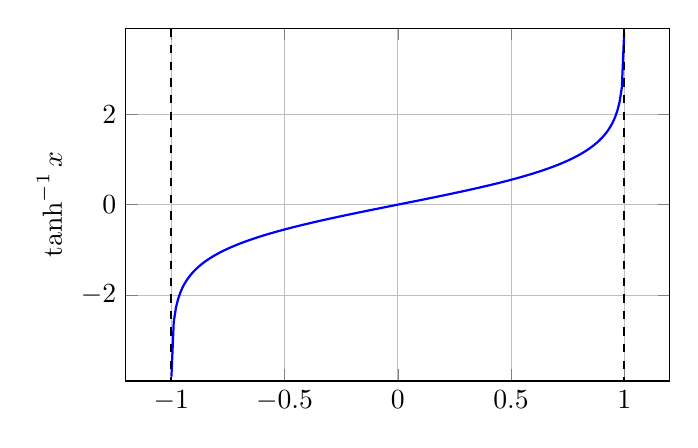
\begin{tikzpicture}
    \pgfkeys{/pgf/declare function={arctanh(\x) = 0.5*(ln((1+\x)/(1-\x)));}}
    \begin{axis}[
      xmin=-1.2, xmax=1.2,
      ymin=-3.9, ymax=3.9,
      samples=200,
      enlarge x limits=false,
      grid=both,
      width=.7\textwidth,
      height=.5\textwidth,
      no markers,
      % axis equal
      ylabel=\(\tanh^{-1} x\),
      % ytick=none,
      ]
      \addplot +[thick,domain=-0.999:0.999] {arctanh(x)};
      \draw [thick,dashed,domain=-0.99:0.99] (1,-4) -- (1,4);
      \draw [thick,dashed,domain=-0.99:0.99] (-1,-4) -- (-1,4);
    \end{axis}
  \end{tikzpicture}
  \caption{\label{fig:arctanh} Plot of \(\tanh^{-1}\), which diverges as the argument goes to \(\pm 1\).}
\end{figure}

Interestingly, there are no restrictions on the parallel tilt, \( t_\parallel \).
The \( \vec{t} \) parametrization of the tilt is conveniently visualized by plotting the \( \vec{t} \)-vector inside a unit sphere, shown in \cref{fig:tiltSphere}.
If the vector is outside the unit sphere, it is a Type-II, if it is inside, it is a Type-I.
Also, if the projection of the vector onto the \(x,y\)-plane is on the unit disk, the Landau level description is valid, if not, the Landau levels collapse.
When the projection is on the unit disc, the system is in the \emph{magnetic} regime, otherwise, we denote it by the \emph{electric} regime.
All Type-I materials may thus be described by Landau levels, while it for Type-II is only valid for certain directions of \(\vec{t}\).
As the \(t\)-vector gets larger, the magnetic regime is restricted to smaller angles between \( \vec{t} \) and \( \vec{B} \).
\begin{figure}[ht]
  \centering
  % \includegraphics[width=0.75\textwidth]{figures/tiltSphere.png}
  % \includegraphics[width=0.75\textwidth]{figures/tiltSpherewactualWhiteBackground.png}
  \iftoggle{full-size-image}{%
    \includegraphics[width=0.75\textwidth]{figures/tiltSpherewBackground}
  }{%
    \includegraphics[width=0.75\textwidth]{figures/tiltSpherewBackground-small}
  }
  \caption{Geometric visualization of the \emph{tilt vector} \( \vec{t} \).
    When the vector is inside the unit sphere (\( t < 1 \)), the system is in the Type-I regime.
    When the vector is outside the unit sphere (\( t > 1 \)), the system is in the Type-II regime.
    When the projection onto the \( xy \)-plane is on the unit disc, the system is in the \emph{magnetic} regime, otherwise, it is in the \emph{electric} regime.
    Shown are Type-I tilt (blue), Type-II magnetic (red), and Type-II electric (green).
    Figure inspired by~\textcite{tchoumakovMagneticFieldInducedRelativisticProperties2016}.
\label{fig:tiltSphere}
  }
\end{figure}

We now return to solving \cref{eq:32}, using the solution angle we just found.
By insertion, and after some clean up, we get
% \emph{note to thorvald: we chose \(\theta = Log \left(+ \dots\right) \)}
% \begin{multline}
%   (R H_{B} R - E R^2 ) \ket{\tilde{\psi}} = 0
%   = v_F\\
%   \times \begin{pmatrix}
%           k_z ( s + t^s_z \gamma ) - E / v_F \gamma & -s ( ik_y + k_z t_x t_z \gamma - k_x / \gamma - E /v_{F} \gamma t^s_x)\\
%           s ( i k_y - k_z t_x t_z \gamma + k_x / \gamma + E /v_F \gamma t^s_x) & - k_z (s - t^s_z \gamma) - E /v_F \gamma
%         \end{pmatrix}
%     \ket{\tilde{\psi}}.
% \end{multline}
\begin{equation}
  \label{eq:39}
  (R H_{B} R - E R^2 ) \ket{\tilde{\psi}}
  = v_F  A \ket{\tilde{\psi}} = 0,
\end{equation}
with
\begin{align*}
  A_{11} &=   k_z ( s + t_{\parallel}^s \gamma ) - E / v_F \gamma,\\
  A_{12} &=  -s ( ik_y + k_z t_\perp t_\parallel \gamma - k_x / \gamma - E /v_{F} \gamma t_{\perp}^s),\\
  A_{21} &= s ( i k_y - k_z t_\perp t_\parallel \gamma + k_x / \gamma + E /v_F \gamma t_{\perp}^s),\\
  A_{22} &= - k_z (s - t_{\parallel}^s \gamma) - E /v_F \gamma.
\end{align*}
In order to simplify this further, absorb \(\gamma t_{\perp}^s (k_{z} t_{\parallel}^s - E /v_{F}) \) into \(k_{x}\).
Thus, let
\begin{equation}
  \label{eq:40}
  \begin{split}
    \tilde{k}_{x} &= k_{x} / \gamma + \gamma t_{\perp}^s ( E /v_F - k_{z} t_{\parallel}^s),\\
    \tilde{k}_{y} &=  k_{y},\\
    \tilde{k}_{z} &=  k_{z}.\\
  \end{split}
\end{equation}

These expressions warrant some explanation, as the Lorentz boost is of course
\begin{equation}
  \label{eq:41}
  \tilde{k}_x = \gamma (k_x - t_{\perp} \frac{E}{v_{F}}),
\end{equation}
where \( E \) is the effective energy, and we used the four momentum \( p^{\mu } = (\frac{E}{v_{F}}, \vec{p}) \), and the effective speed of light \( v_F \).
It can thus look like our expression in \cref{eq:40} is wrong.
The solution to this seeming inconsistency is that the proper effective energy is not \( E - v_F k_z t^{s}_{\parallel} \), but rather \( E  - v_F k_z t^{s}_{\parallel} - v_F k_x t^{s}_{\perp}\)~\cite{yuPredictedUnusualMagnetoresponse2016}.

The eigenvalue equation in the transformed momenta is simply
\begin{equation}
  \label{eq:42}
  \left[  \gamma \left( t^s_{\parallel} \tilde{k}_{z} - \frac{E}{v_{F}} \right) \mathcal{I}_{2} +
  s \tilde{k}_{i} \sigma _{i} \right] \ket{\tilde{\psi}}= 0.
\end{equation}
If we now again introduce the magnetic field using minimal coupling, \(k_{x} \to  k_{x} - ey B_{z} \), this corresponds to an effective field \(B_{z} /\gamma \) in the new quantities.
This is because \(\tilde{k}_{x} \to  \tilde{k}_{x} - e y B_{z} /\gamma \).
The Landau level equation thus reads
\begin{equation}
  \label{eq:43}
  \left[
  \sum\limits_{i} s v_{F} \left(\tilde{k}_{i} + e \tilde{A}_{i} \right) \sigma _{i}
\right  ] \ket{\tilde{\psi}} =
(E- t^s_{\parallel} v_{F} \tilde{k}_{z}) \gamma \ket{\tilde{\psi}},
\end{equation}
where \(\vec{\tilde{A}}=-B_{z}/ \gamma y \hat{x}\).
We may thus use directly the result for the untilted cone, \cref{eq:26}, giving
\begin{subequations}
  \label{eq:44}
  \begin{align}
    \left(E - t^s_{\parallel} v_{F} \tilde{k}_{z} \right) \gamma &= \sign (m) v_{F} \sqrt{2 |m| e \frac{B}{ \gamma }  + \tilde{k}_{z}^2}, & m \neq 0,\\
    \left(E - t^s_{\parallel} v_{F} \tilde{k}_{z} \right) \gamma &= - s   \tilde{k}_{z} v_{F}, & m=0.
  \end{align}
\end{subequations}
Cleaning up and introducing explicitly the quantum numbers to the energy
\begin{subequations}
  \label{eq:45}
  \begin{align}
    E_{k_z m s} &= t^s_{\parallel} v_F \tilde{k}_{z} + \sign(m) \frac{v_F}{\gamma} \sqrt{2 |m| e \frac{B}{\gamma}  + \tilde{k}_{z}^2}, & m\neq 0,\\
    E_{k_z 0 s} &= \tilde{k}_{z} v_{F} \left( t^s_{\parallel}  - s  / \gamma  \right), & m=0.
  \end{align}
\end{subequations}

As the perpendicular tilt is increased, \(\gamma = 1 / \sqrt{1-t_{\perp} ^{2}}\) diverges to infinity.
With the trivial substitution \(\alpha = 1 /\gamma \), which goes to zero, this gets an intuitive interpretation.
As the perpendicular tilt increases, the Landau levels converge towards \(t_{\parallel} v_{F} \tilde{k}_{z}\).
In particular, the separation between Landau levels is reduced by a factor \(\alpha ^{3 /2}\).
The effect of the tilt on the Landau levels is to squeeze the Landau levels together, and we will call the \(\alpha \) the \emph{squeezing factor}.
We note that when approaching the degree of tilt where we are no longer able to find a boost that enables us to solve for the Landau levels, i.e. when \( |t_{\perp}| \to 1\), the squeezing factor goes to zero.
As the tilt exceeds this limit, the squeezing factor is imaginary.
% The Landau level description is only valid for \( |t_{\perp}| < 1 \).

The energy levels of the tilted cone expressed in terms of the energy levels of the untilted cone
\[
E_{k_z m s} = t^s_{\parallel} v_F k_z + \alpha E^0_{m, \alpha B},
\]
where \( E^0_{m, \alpha B} \) is the energy in the untilted case, with magnetic field \( \alpha B \).
Tilting of the Landau levels is induced by the parallel tilt component, \( t_\parallel \).
The Landau levels cross the Fermi level at the transition from Type-I to Type-II as well.
The Landau levels are shown in \cref{fig:llevelstilt}.


\begin{figure}[p!]
  \centering
  \resizebox{\textwidth}{!}{
  \newcommand{\LLplot}[2]{
  %% #1 is alpha, #2 is tz
  \addplot[forget plot]{(#2-#1) * x};  % Zeroth level
  \addplot[forget plot, black!60, dash pattern={on 3pt off 2pt on 1pt off 2pt on 1pt off 2pt on 1pt off 2pt}]{(-#2+#1) * x};  % Zeroth level, s=-1
  \addplot[forget plot, dashed]{(#2+#1) * x};  % Zeroth level, s=-1, P broken
  \addplot[forget plot, dotted]{(-#2-#1) * x};  % Zeroth level, s=1, tz<1
  \addplot[dashed, forget plot, gray] {0};
  \pgfplotsforeachungrouped \n in {1,...,5} {
    \addplot+[red, forget plot, solid] {#2 * x + #1 * sqrt(\n * #1 + x^2)};  % Positive E
    \addplot+[blue, solid] {#2 * x - #1 * sqrt(\n * #1 + x^2)};  % Negative E
  }
  \pgfplotsforeachungrouped \n in {1,...,5} {
    \addplot+[red, forget plot, dotted] {-#2 * x + #1 * sqrt(\n * #1 + x^2)};  % Positive E
    \addplot+[blue, dotted] {-#2 * x - #1 * sqrt(\n * #1 + x^2)};  % Negative E
  }
}

\tikzsetnextfilename{lllevels}
%% \hspace{-1.6cm}
\begin{tikzpicture}
  \begin{groupplot} [%
    width=0.5\textwidth, %% Width of each window... Can be set more elegantly, but here just trial and error
    cycle list name=linestyles,
    samples=100,
    ymin=-2.5,ymax=2.5,
    xmin=-3.9, xmax=3.9,
    xlabel=\( \kappa_z \),
    ylabel=\( \epsilon_{\kappa_z m s} \),
    group style={
      x descriptions at=edge bottom,
      y descriptions at=edge left,
      horizontal sep=4pt, vertical sep=4pt,
      group size=2 by 3,
    },
    ]
    \newcommand\varalpha{1}
    \newcommand\vartz{0}
    %%
    \nextgroupplot
    \LLplot{\varalpha}{\vartz}
    \pgfmathsetmacro\hfirst{\vartz-\varalpha}
    \pgfmathsetmacro\hsecond{\vartz * 1 + \varalpha * sqrt(\varalpha + 1)}
    \draw[->] (axis cs:1,\hfirst)--(axis cs:1, \hsecond);
    %%
    \nextgroupplot
    \renewcommand\varalpha{0.6}
    \renewcommand\vartz{0}
    \LLplot{\varalpha}{\vartz}
    \pgfmathsetmacro\hfirst{\vartz-\varalpha}
    \pgfmathsetmacro\hsecond{\vartz * 1 + \varalpha * sqrt(\varalpha + 1)}
    \draw[->] (axis cs:1,\hfirst)--(axis cs:1, \hsecond);
    %%

    \nextgroupplot
    \renewcommand\varalpha{1}
    \renewcommand\vartz{0.5}
    \LLplot{\varalpha}{\vartz}
    \pgfmathsetmacro\hfirst{\vartz-\varalpha}
    \pgfmathsetmacro\hsecond{\vartz * 1 + \varalpha * sqrt(\varalpha + 1)}
    \draw[->] (axis cs:1,\hfirst)--(axis cs:1, \hsecond);
    %%
    \nextgroupplot
    \renewcommand\varalpha{0.6}
    \renewcommand\vartz{0.5}
    \LLplot{\varalpha}{\vartz}
    \pgfmathsetmacro\hfirst{\vartz-\varalpha}
    \pgfmathsetmacro\hsecond{\vartz * 1 + \varalpha * sqrt(\varalpha + 1)}
    \draw[->] (axis cs:1,\hfirst)--(axis cs:1, \hsecond);

    \pgfmathsetmacro\x{-0.8}
    \pgfmathsetmacro\gfirst{\vartz * \x - \varalpha * sqrt(1 * \varalpha + (\x)^2)}
    \pgfmathsetmacro\gsecond{\vartz * \x + \varalpha * sqrt(4 * \varalpha + (\x)^2)}
    \draw[brown, ->] (axis cs:\x,\gfirst)--(axis cs:\x, \gsecond);  %% Higher order transition
    %%
    \nextgroupplot
    \renewcommand\varalpha{1}
    \renewcommand\vartz{1.2}
    \pgfmathsetmacro\x{-sqrt(\varalpha^2/(\vartz^2-\varalpha^2))-0.3}
    \LLplot{\varalpha}{\vartz}
    \pgfmathsetmacro\hfirst{\vartz * \x + \varalpha * sqrt(\varalpha + (\x)^2)}
    \pgfmathsetmacro\hsecond{\vartz * \x + \varalpha * sqrt(2 * \varalpha + (\x)^2)}
    \draw[teal!80!black, ->, thick] (axis cs:\x,\hfirst)--(axis cs:\x, \hsecond);  %% Intraband
    %%
    \nextgroupplot
    \renewcommand\varalpha{0.6}
    \renewcommand\vartz{1.2}
    \pgfmathsetmacro\x{-sqrt(\varalpha^2/(\vartz^2-\varalpha^2))/2}
    \LLplot{\varalpha}{\vartz}
    \pgfmathsetmacro\hfirst{(\vartz - \varalpha) * \x}
    \pgfmathsetmacro\hsecond{\vartz * \x + \varalpha * sqrt(1 * \varalpha + (\x)^2)}
    \draw[->] (axis cs:\x,\hfirst)--(axis cs:\x,\hsecond);
  \end{groupplot}
\end{tikzpicture}

  }
  % \includegraphics[width=0.8\textwidth]{example-image-10x16}
  \caption{\label{fig:llevelstilt}Landau levels for different values of \( t_\perp, t_\parallel \).
    The top two rows show Type-I, while the lowest row shows Type-II.
    Left column shows \( t_\perp = 0 \), right column \( t_\perp = 0.64 \) (\( \alpha = 0.6 \)).
    The rows show \( t_\parallel = 0, 0.5, 1.2 \), from top to bottom.
    The dotted lines show the Landau levels with opposite sign of \( t_\parallel \), the dashed show the opposite chirality.
    The arrows indicate valid ``transitions'', namely the \( 0\to 1 \) interband in black, \( -1 \to 4 \) interband in \textcolor{brown!70!black}{brown}, and \( 1\to 2 \) intraband in \textcolor{teal!70!black}{teal}.
    See main text for details.
  }
\end{figure}

The eigenstate of
\[
H = v_{F} \sigma ^{i} ( p_{i} + e A_{i} ),
\]
with \(A_{i} = - B_{z} y \delta _{i x}\), as given in summary \ref{summary:ll-notilt} using the position basis,
\begin{equation*}
  \phi _{\vec{k} m s}(\vec{r}) =  \frac{e^{ik_x x}e^{ik_z z}}{\sqrt{L_xL_z}}
  \frac{e^{-\frac{(y-k_x l^2)^2}{2 l_B^2}}}{\sqrt{\alpha_{k_z m s}^2 + 1}}
  \begin{pmatrix}
    \frac{\alpha_{k_z m s}}{\sqrt{2^{M-1} (M-1)! \sqrt{\pi } l_B}} H_{M-1}\left( \frac{y-k_x l_B^2}{l_B} \right)\\
    \frac{1}{\sqrt{2^M M! \sqrt{\pi } l_B}} H_M \left( \frac{y-k_x l_B^2}{l_B} \right)
  \end{pmatrix},
\end{equation*}
where capital letters indicate absolute value of corresponding quantity, $M=|m|, \vec{k} = (k_x, k_z)$, and with the normalization factor
\begin{equation}
  \alpha_{k_z m s} = \frac{-\sqrt{2eB M}}{\frac{E_{k_z m s}}{s v_{F}} -   k_z}.
\end{equation}
Taking care to keep track of boosted and rescaled quantities, the eigenstate in the boosted frame is
\begin{equation}
  \label{eq:47}
  \tilde{\phi}(\tilde{\vec{r}}) =
  \frac{e^{i \tilde{k}_x \tilde{x}}e^{i k_z z}}{\sqrt{L_xL_z}}
  \frac{e^{-\frac{\left(\tilde{y} - \tilde{k}_x l_{B'}^2\right)^2}{2 l_{B'}^2}}}{\sqrt{\alpha_{\tilde{k}_z m s}^2 + 1}}
  \begin{pmatrix}
    \frac{\alpha_{\tilde{k}_z m s}}{\sqrt{2^{M-1} (M-1)! \sqrt{\pi } l_{B'}}} H_{M-1}\left( \frac{\tilde{y} - \tilde{k}_x l_{B'}^2}{l_{B'}} \right)\\
    \frac{1}{\sqrt{2^M M! \sqrt{\pi } l_{B'}}} H_M \left( \frac{\tilde{y} - \tilde{k}_x l_{B'}^2}{l_{B'}} \right)
  \end{pmatrix},
\end{equation}
with
\begin{equation}
  \alpha_{\tilde{k}_z m s} = \frac{-\sqrt{2e B'  M}}{ \gamma \frac{E_{\tilde{k}_z m s} - t^s_{\parallel} v_{F} \tilde{k}_{z}}{s v_{F}} -   \tilde{k}_z},
\end{equation}
where
\[
B' = B \alpha.
\]
We note that \( \alpha_{k_z 0 s} = 0 \), so using the explicit form of the energy we may simplify the expression some.
For \( m\neq 0 \)
\[
  \frac{
    E_{k_z m s} - t^s_{\parallel} v_F k_z
  }{s v_{F}} = \sign(m) s \alpha \sqrt{2 M e B \alpha + k_{z}^2}
\]
and thus
\begin{equation}
  \label{eq:48}
  \alpha_{k_z m s} =
  \frac{-\sqrt{ \alpha M }}{\sign(m) s \sqrt{\alpha M + \kappa^2} - \kappa}
\end{equation}
where we defined the dimensionless \( \kappa_z = \sqrt{2 e B} k_z  \).

The original eigenstate \(\ket{\psi } = 1 /\mathcal{N} e^{\theta /2 \sigma _{x}} \ket{\tilde{\psi} }\) of the tilted system is easily found.
Reinserting explicitly, in the boosted frame, that
\[
  \tilde{k}_{x} = \alpha k_{x} + \frac{t_{\perp}^s}{\alpha} (E_{k_z m s} /v_F- k_{z} t_{\parallel}^s)
  = \alpha k_x + t_{\perp}^s \frac{E^0_{m, \alpha B} }{v_{F}}
\]
and \(l_{B'}=\frac{l_{B}}{\sqrt{\alpha} }\)
we define
\begin{equation}
  \label{eq:49}
  \chi =
  \frac{y-\tilde{k}_{x} l_{B'}^2}{l_{B'}}
  =
  \sqrt{\alpha } (y-k_{x} l_{B}^2) /l_{B}
  + \frac{ t_{\perp}^s l_B }{ \sqrt{\alpha} v_F} E^{0}_{m, \alpha B},
\end{equation}
which is the argument of the Hermite polynomials.
For later convenience, let us explicitly define
\begin{equation}
  \label{eq:50}
  \tilde{\phi} _{\vec{k} m s} (\vec{\tilde{r}}) =
  \frac{e^{i \tilde{k}_{x} \tilde{x} + i k_{z} z}}{\sqrt{L_{x} L_{z}} }
  \underbrace{
  \frac{
    e^{-\frac{1}{2} \chi ^2}
    \sqrt[4]{\alpha }
  }
  {\sqrt{\alpha^2_{\tilde{k}_{z} m s} + 1} }
  \begin{pmatrix}
    \frac{\alpha_{\tilde{k}_z m s}}{\sqrt{2^{M-1} (M-1)! \sqrt{\pi } l_{B}}} H_{M-1}\left( \chi  \right)\\
    \frac{1}{\sqrt{2^M M! \sqrt{\pi } l_{B}}} H_M \left( \chi \right)
  \end{pmatrix}}_{\tilde{\phi}_{\vec{k} m s} (y)},
\end{equation}
and thus
\begin{equation}
  \label{eq:51}
  \tilde{\phi}_{\vec{k} m s} (y) =
  e^{-\frac{1}{2} \chi ^2}
  \begin{pmatrix}
    a_{\vec{k} m s} H_{M-1} (\chi)\\
    b_{\vec{k} m s} H_{M} (\chi)
  \end{pmatrix},
\end{equation}
with
\begin{align}
 \label{eq:52}
  a_{\vec{k} m s} &=
                    \frac{
                    \alpha_{\tilde{k}_z m s} \sqrt[4]{\alpha }
                    }{
                    \sqrt{\alpha^2 _{\tilde{k}_z m s} + 1}
                    \sqrt{2^{M-1} (M-1)! \sqrt{\pi} l_B}
                    },\\
  \label{eq:53}
  b_{\vec{k} m s} &=
                    \frac{
                     \sqrt[4]{\alpha }
                    }{
                    \sqrt{\alpha^2 _{\tilde{k}_z m s} + 1}
                    \sqrt{2^{M} M! \sqrt{\pi} l_B}
                    }.
\end{align}

We proceed now to find the normalization factor \( \mathcal{N} \), as it will become necessary in later steps.
Recall that
\[
  \ket{\psi} = \frac{1}{\mathcal{N}} e^{\theta /2 \sigma _x} \ket{\tilde{\psi}},
\]
and use that for \( \theta = \tanh^{-1}(-s t^s_{\perp}) \) the hyperbolic rotation
\[
  R^2 =
e^{\theta \sigma _x} =
\frac{1}{\alpha }
\begin{pmatrix}
  1 & -s t_{\perp}^s\\
  -s t_{\perp}^s & 1
\end{pmatrix}.
\]
The upper and lower part of the spinor are orthogonal, thus we have
\begin{equation}
  \label{eq:54}
  \braket{\psi  | \psi } = \frac{1}{\mathcal{N}^{*} \mathcal{N}} \frac{1}{\alpha } \braket{\tilde{\psi}  | \tilde{\psi} } = 1 \implies \mathcal{N}^{*}\mathcal{N} = \frac{1}{\alpha }.
\end{equation}
We choose \( \mathcal{N} = \alpha^{-\frac{1}{2}} \).

\begin{summary}\label{summary:llevels}
The tilted Hamiltonian
  \[
    H = v_F \vec{t}^s \vec{p} + s v_F \vec{p} \vec{\sigma}
  \]
  in a magnetic field \( \vec{B} \) has the Landau levels
  \[
    E =
    \begin{cases}
      t^s_{\parallel} v_F k_z + \sign(m) v_F \alpha \sqrt{2 e B \alpha M + k_{z} ^2} & m \neq 0,\\
      t^s_{\parallel} v_F k_z - s \alpha v_F k_z & m = 0,
    \end{cases}
  \]
  with the \emph{squeezing factor} \( \alpha = \sqrt{1 - t_{\perp} ^2}  \).
  The associated eigenstates in the position basis are
  \[
    \psi(\vec{r}) = \sqrt{\alpha} e^{\theta /2 \sigma_x}
    \frac{
      e^{ik_{x} x + ik_{z} z}
    }{
      \sqrt{L_{x}  L_z}
    } \tilde{\psi}(y),
    \]
    where
    \[
      \tilde{\psi} (y) = e^{-\frac{1}{2} \chi^2}
      \begin{pmatrix}
        a_{k_z m s} H_{M - 1} (\chi) \\
        b_{k_z m s} H_M (\chi)
      \end{pmatrix},
    \]
    where we have defined \( \chi = \sqrt{\alpha} \frac{ y - k_x l_B^2 }{l_{B}} + \frac{t_{\perp}^s l_B}{\sqrt{\alpha} v_{F}} E^0_{m, \alpha B} \) and \( a_{k_z m s}, b_{k_z m s} \) are given in \cref{eq:52,eq:53}.
\end{summary}

We will find the current response of a single Dirac cone, with a temperature gradient $\nabla_y T$ and a magnetic field $B_z$.
The current response of interest in the given geometry is thus in the $x$-direction,
\begin{equation}\label{eq:1}
  J^x = \chi ^{xy} \frac{- \nabla _yT}{T},
\end{equation}
with $\chi^{xy}$  being the response\footnote{The sign in Eq. (\ref{eq:1}) depends on the choice of the response function being the response of the gravitational potential or the temperature gradient. Thus, the sign may differ in the literature.}.
In the derivation of~\citeauthor{chernodubGenerationNernstCurrent2018}~\cite{chernodubGenerationNernstCurrent2018} the response
\begin{equation}
  \chi ^{xy} = \frac{e^2 v_F B}{18 \pi ^2 \hbar }
\end{equation}
was found, while the derivation of~\citeauthor{arjonaFingerprintsConformalAnomaly2019}~\cite{arjonaFingerprintsConformalAnomaly2019} found
\footnote{The paper is somewhat unclear on what is their final result, as there is some possible confusion related to the number of Landau levels included and whether one is including both or only one Dirac cone.
The above result is what is meant, to the best of our understanding.}
\begin{equation}
  \chi ^{xy} = \frac{e^2 v_F B}{4 \pi ^2 \hbar }.
\end{equation}

Recall the linear response from the Kubo formalism in Eq. (\ref{eq:99current-luttinger-gravity-final}), found through Luttinger's approach.
\begin{equation}
  \label{eq:2}
  \braket{J^i}(t, \vec{r}) =
  \int\limits_{-\infty }^{\infty } \mathrm{d}t' \mathrm{d}\vec{r}'
  \int\limits_{-\infty }^{t'} \mathrm{d}t''
  \left\{
    \frac{-i v_F}{\hbar } \Theta (t-t')
    \Braket{
      [J^i(t, \vec{r}), T^{0j} (t'', \vec{r}')]
    }
  \right\}
  \partial _j' \psi (t', \vec{r}').
\end{equation}
Fourier transforming now to the frequency and momentum domain, will be beneficial in our calculations.
As before, the non-perturbed system will be taken to be time and position invariant, such that the correlator in Eq. (\ref{eq:2}) can be taken to depend only on the differences $t-t''$ and $\vec{r} - \vec{r}' $.
Starting with Fourier transforming the position part, notice that the structure of Eq. (\ref{eq:2}) is
\[
  \braket{J^i}(\vec{r}) = \int \mathrm{d} \vec{r}' \chi (\vec{r} - \vec{r}') \partial _j' \psi  (\vec{r}'),
\]
where the temporal parts were dropped for clarity.
This is a convolution, and the Fourier transform is thus simply given by the product of the two factors~\cite{rottmannMatematiskFormelsamling1995}.
\begin{equation}
  \braket{J^i}(\vec{q}) =
  \chi (\vec{q}) (iq_j) \psi (\vec{q}),
\end{equation}
where it was also used that the Fourier transform of a derivative gives the component of the variable.
Showing explicitly how to find the form of the response $\chi $ in momentum space is often overlooked in much literature, and as it does involve some finesse, we want to show it here.
This trick is courtesy of~\citeauthor{changLectureNotesManybody2018}~\cite{changLectureNotesManybody2018}.
By definition, the Fourier transform of the response is, where the variable of integration has been chosen to be $\vec{r}-\vec{r}'$ for later convenience,
\begin{align}
  \chi (\vec{q}) &= \int \mathrm{d}(\vec{r} - \vec{r}') e^{-i\vec{q}(\vec{r}-\vec{r}')} \chi (\vec{r} - \vec{r}')\\
                 &= \int \mathrm{d}(\vec{r} - \vec{r}') e^{-i\vec{q}(\vec{r}-\vec{r}')} C \Braket{
                   \left[
J^i (\vec{r}), T^{0j}(\vec{r}')
                   \right]},\\
\end{align}
where $C$ denotes $t$-dependent prefactors and integrals over time are omitted, again for clarity of notation.
Note that
\begin{equation}
  \int \mathrm{d}(\vec{r} - \vec{r}') = \frac{1}{\mathcal{V}} \int \mathrm{d}\vec{r} \mathrm{d} \vec{r}',
\end{equation}
where $\mathcal{V}$ is the volume of the system.
Thus,
\begin{equation}
  \begin{split}
    \chi (\vec{q}) &= \frac{1}{\mathcal{V}} \int \mathrm{d}\vec{r} \mathrm{d}\vec{r}'
    e^{-i\vec{q}(\vec{r}-\vec{r}')}
    C \Braket{\left[
        J^i(\vec{r}), T^{0j}(\vec{r}')
      \right]}\\
    &= \frac{C}{\mathcal{V}} \Braket{\left[ J^i(\vec{q}), T^{0j}(-\vec{q}) \right]}.
  \end{split}
\end{equation}

Considering now the temporal part, the procedure is simpler.
The linear response still has the form of a convolution, as the response function is only dependent on the difference $t-t'$ by
\begin{equation}
  \chi (t-t') = \int\limits_{-\infty }^0 \mathrm{d} t'' \Theta (t - t')
  \Braket{\left[ J(t-t'), T(t'') \right]},
\end{equation}
where $t''$ was shifted by $t' $, and then the translational invariance of the correlator was used.
In frequency space
\begin{align}
  \chi (\omega ) &= \int \mathrm{d} t e^{i \omega  t} \chi (t)\\
                 &= \int \mathrm{d} t e^{i \omega  t} \int\limits_{-\infty  }^0 \mathrm{d} t''
                   \Theta (t) \Braket{\left[ J(t), T(t'') \right]}.
\end{align}
In frequency and momentum space the response function is thus
\begin{equation}\label{eq:3}
  \chi ^{ij} (w, \vec{q}) =
  \frac{-iv_F}{\mathcal{V} \hbar } 
  \int \mathrm{d}t e^{i\omega t}
  \int\limits_{-\infty }^{0} \mathrm{d}t'
  \Theta (t)
  \Braket{\left[
      J^i(t, \vec{q}), T^{0j}(t', -\vec{q})
    \right]}.
\end{equation}

\section{Eigenvalue problem of the Landau levels of a Weyl Hamiltonian}
To evaluate the correlator of the response function, the matrix elements of the current and stress-energy tensor must be found.
In order to do this, we find eigenstates in the Landau basis of the system.
The Weyl Hamiltonian
\begin{equation}
  \label{eq:99weyl-hamil}
  H_s = s v_F \sigma^i \left( p_i + e A_i \right),
\end{equation}
with $s$ being the chirality, $p_i$ the momentum operator, and $e = |e|$ the coupling constant to the electromagnetic field $\vec{A}$.
Choose coordinates such that $\vec{B} = B_z \hat{\vec{z}}$, which in the Landau gauge gives $\vec{A} = -B_{z}y \: \hat{\vec{x}}$.
As the Hamiltonian is invariant in $x$ and $z$, take the plane wave ansatz $\phi(\vec{r}) = e^{ik_x x + i k_z z} \phi (y)$.
It then follows
\begin{equation}
  H_s \phi(\vec{r}) = E \phi(\vec{r}) \implies \tilde{H}_s \phi(y)  = E \phi(y),
\end{equation}
where $\tilde{H}$ is the result of replacing $p_z \to \hbar k_z, p_x\to \hbar  k_x$ in $H_s$, as the plane wave part of $\phi $ have these eigenvalues.
Absorb the chirality $s$ as a sign in the velocity $v_F$, for more concise notation. 
Thus, writing everything explicitly, the spectrum is given by
\begin{equation}
  \label{eq:4}
  -\hbar  v_F
  \begin{pmatrix}
    - k_z & \partial _y + e y B_{z} / \hbar  - k_x\\
    -\partial _y + e y B_{z} / \hbar -k_x & k_z
  \end{pmatrix}
  \phi(y)  = E\phi(y).
\end{equation}
We will now find the spectrum $E$ of the Hamiltonian.

Inspired by the derivation for the spectrum of the 2D Dirac Hamiltonian in~\cite{wehlingDiracMaterials2014}, we introduce the length scale $l_B = \sqrt{\hbar / eB}$, and the dimensionless quantity $\chi = y /l_{B} - k_x l_{B}$.
In dimensionless quantities Eq. (\ref{eq:4}) becomes
\begin{equation}
  -\frac{{\hbar v_F}}{l_{B}}
  \begin{pmatrix}
    -k_z l_B & \partial _{\chi } + \chi \\
    -\partial _{\chi } + \chi & k_z l_B
  \end{pmatrix}
  \phi(y)  =  E \phi(y).
\end{equation}
Let the operators \(a = \left( \chi + \partial _{\chi } \right) / \sqrt{2},\; a^{\dagger} = \left( \chi - \partial _{\chi } \right) /\sqrt{2}\).
One may easily verify the commutation relation $[a, a^{\dagger}] = 1$;
they are ladder operators of the harmonic oscillators, whose eigenstates are $\ket{n}$, and where $a\ket{n} = \sqrt{n}\ket{n-1}, a^{\dagger} \ket{n} = \sqrt{n+1} \ket{n+1}$.
In terms of these operators, the system is
\begin{equation}
  -\frac{\sqrt{2} \hbar v_F}{l_B}
  \begin{pmatrix}
    -\frac{k_zl_B}{\sqrt{2}} & a\\
    a^{\dagger} & \frac{k_zl_B}{\sqrt{2}}
  \end{pmatrix}
  \ket{\phi } = E \ket{\phi }.
\end{equation}
Take the ansatz
\begin{equation}
  \ket{\phi } =
  \begin{pmatrix}
    \beta \ket{n-1}\\
    \alpha  \ket{n}
  \end{pmatrix},
\end{equation}
which is the most general form of $\ket{\phi }$ with any hope of being an eigenstate.
This leads to
\begin{equation}
  -\frac{\sqrt{2} \hbar v_F}{l_B}
  \begin{pmatrix}
    \left( -\gamma \beta + \alpha \sqrt{n} \right) \ket{n-1}\\
    \left( \beta \sqrt{n} + \gamma \alpha \right) \ket{n}
  \end{pmatrix}
  = E \ket{\phi },
\end{equation}
with $\gamma  = k_zl_B / \sqrt{2}$.
For $n > 0$ this leads to the equation for $\phi $ to be an energy eigenfunction
\begin{equation}
  -\gamma + \frac{\alpha}{\beta } \sqrt{n} = \frac{\beta }{\alpha } \sqrt{n} + \gamma.
\end{equation}
Solving for $\alpha /\beta $ this gives
\begin{equation}
  \frac{\alpha}{\beta } = \frac{\gamma}{\sqrt{n}} \pm \sqrt{1 + \frac{\gamma^2}{n}},
\end{equation}
and thus
\begin{equation}
  E = \pm v_F \sqrt{
    \frac{2n \hbar ^2}{l_B^2} + k_z^2\hbar ^2
  }
  = \pm s v_F \sqrt{
    2n e B \hbar + k_z^2\hbar ^2
  },
\end{equation}
where we reintroduced the explicit $s$.
For $n = 0$ the annihilation operator $a$ destroys the vacuum state $\ket{0}$, and the energy is instead $E_0 = -\hbar s k_z v_F$.
The excited energy states are doubly degenerate;
we choose to denote the energy levels by $m \in \mathbb{Z}$, where the sign from $\pm s$ is taken care of by the sign of this quantum number, and the harmonic oscillator levels $n$ are given by its absolute value $|m|$.
The energy levels are
\begin{align}
  E_{k_z m s} &= \operatorname{sign}(m) v_F \sqrt{2 |m| e B \hbar  + k_z^2 \hbar ^2} & \text{ for } m \neq 0,\\
E_{k_z 0 s} &= -s \hbar k_z v_F & \text{ for } m = 0.
\end{align}

We now find the corresponding eigenvectors of the system.
The solution to the one dimensional harmonic oscillator in position space is, in dimensionless coordinates $\xi$,~\cite[Eq.~18.39.5]{NIST:DLMF}
\begin{equation}
  \braket{\xi | n} = \phi _n (\xi)
  = \frac{1}{\sqrt{2^nn!}} \pi^{-\frac{1}{4}}
  e^{- \frac{\xi^2}{2}} H_n \left( \xi \right),
  % = \frac{1}{\sqrt{2^nn!}} \left( m\frac{\omega}{\pi \hbar } \right)^{\frac{1}{4}}
  % e^{- \frac{{m\omega x^2}}{2\hbar }} H_n \left( \sqrt{\frac{m\omega }{\hbar } x} \right),
\end{equation}
where $H_n$ are the Hermite polynomials.
Thus,
\begin{equation}
  \braket{\chi | \phi } =
  \begin{pmatrix}
    \beta \braket{\chi | n-1}\\
    \alpha \braket{\chi | n}
  \end{pmatrix}
  =
  e^{- \frac{\chi^2}{2}}
  \begin{pmatrix}
    \frac{\beta }{\sqrt{2^{n-1}(n-1)!\sqrt{\pi }}} H_{n-1} \left( \chi \right)\\
    \frac{\alpha }{\sqrt{2^{n}n!\sqrt{\pi }}} H_n \left(\chi \right)\\
  \end{pmatrix}
\end{equation}
Choosing
\begin{equation}
  \alpha  = \sqrt{\frac{\gamma^2}{n}} \implies \beta = \frac{1}{1 \pm \sqrt{1 + \frac{n}{\gamma ^2}}} = \pm \frac{\gamma ^2}{n} \left( \sqrt{1 + \frac{n}{\gamma ^2}} - 1 \right),
\end{equation}
gives
\begin{equation}
  \phi (\chi ) = e^{-\frac{\chi^2}{2}} \sqrt{\frac{\gamma ^2}{n}}
  \begin{pmatrix}
    \frac{
      \pm \sqrt{\frac{\gamma ^2}{n}} \left( \sqrt{1 + \frac{n}{\gamma ^2}} - 1 \right)
    }{
      \sqrt{2^{n-1} (n-1)! \sqrt{\pi }}
    }
    H_{n-1}(\chi )\\
    \frac{1}{\sqrt{2^{n}n!\sqrt{\pi }}} H_n \left(\chi \right)
  \end{pmatrix}.
\end{equation}
There are thus four quantum numbers related to the eigenvectors, $k_x,  k_z, m, s$.
Reintroducing $\chi = (y-k_xl_B^2) /l_B$ and normalizing
\begin{equation}
  \phi _{\vec{k} m s}(\vec{r}) = \frac{1}{\sqrt{L_xL_z}}
  \frac{e^{ik_x x}e^{ik_z z}}{\sqrt{\alpha _{k_z m s}^2 + 1}}
  e^{-\frac{\left(y-k_x l^2\right)^2}{2 l_B^2}}
  \begin{pmatrix}
    \frac{\alpha _{k_z m s}}{\sqrt{2^{M-1} (M-1)! \sqrt{\pi } l_B}} H_{M-1}\left( \frac{y-k_x l_B^2}{l_B} \right)\\
    \frac{1}{\sqrt{2^M M! \sqrt{\pi } l_B}} H_M \left( \frac{y-k_x l_B^2}{l_B} \right)
  \end{pmatrix},
\end{equation}
where capital letters indicate absolute value of corresponding quantity, $M=|m|, \vec{k} = (k_x, k_z)$, and with the normalization factor
\begin{equation}
  \alpha _{k_z m s} = \frac{-\sqrt{2eB\hbar M}}{\frac{E_{k_z m s}}{s v_{F}} - \hbar  k_z}.
\end{equation}

\section{Analytical expressions for the operators}
We will here find analytical expressions for the current operator $J^i(\omega, \vec{q})$ and stress-energy tensor $T^{0j}(\omega, \vec{q})$, needed to calculate the correlation function.
The fields are given, in the position basis, by
\begin{align}
  \psi &= \sum\limits_{\vec{k}n}^{}\braket{\vec{r} | \vec{k} n s} a_{\vec{k}ns}(t) = \sum\limits_{\vec{k}n}^{} \phi_{\vec{k} n s} (\vec{r}) a_{\vec{k}n s}(t),\\
  \psi^{\dagger} &= \sum\limits_{\vec{k}n}^{}
                   \braket{\vec{k} ns | \vec{r} }
                   a^{\dagger}_{\vec{k}ns}(t)
                   =\sum\limits_{\vec{k}n}^{} \phi^{*}_{\vec{k} n s} (\vec{r}) a^{\dagger}_{\vec{k}n s}(t).
\end{align}
Here $a_{\lambda }^{\dagger} (t) = \exp(iE_{\lambda } t / \hbar) a_{\lambda }^{\dagger}$ and $a_{\lambda }^{\dagger}, a_{\lambda }$ are the creation and annihilation operators of the state with quantum numbers $\lambda $.
The current operator $\hat{\vec{J}} = e \hat{\vec{v}}$, where $\hat{\vec{v}}$ is the velocity operator.
Using the relation of Heisenberg operators $\dot{A} = [A, H] / i\hbar $~\cite{sakuraiModernQuantumMechanics2017}, for the operator $A$ and Hamiltonian $H$, the operator
\begin{align}
  \vec{v} = \dot{\vec{r}} &= \frac{1}{i \hbar } \left[ \vec{\vec{r}}, H \right]\\
              &= \frac{sv_F \sigma ^i}{i \hbar } \left[ \vec{r}, p_i + e A_i \right]\\
              &= \frac{s v_F \sigma^i }{i \hbar } \left( i\hbar + e[\vec{r}, A_i] \right)\\
              &=s v_F \sigma ^i,
\end{align}
and thus
\begin{equation}
  J^x = \psi ^{\dagger} \hat{J}^x \psi = sv_F e \sum\limits_{\vec{k}m, \vec{l}n}^{}
  \phi _{\vec{k}ms}^{*}(\vec{r}) \sigma ^x \phi _{\vec{l}ns}(\vec{r})
  a_{\vec{k}ms}^{\dagger}(t)
  a_{\vec{l}ns}(t).
\end{equation}
Similarly, the $T^{0y}$ component of the stress-energy tensor of the theory is given by~\cite{arjonaFingerprintsConformalAnomaly2019}
\begin{equation}
  \begin{split}
    T^{0y}(t, \vec{r}) &=
    \sum\limits_{\vec{k} m, \vec{l} n}^{}
    \frac{1}{4}
    \bigg\{
    \left[
      v_F \phi ^{*}_{\vec{k} m s}(\vec{r}) p_y \phi _{\vec{l} n s}(\vec{r})
      -v_F \left( p_y \phi ^{*}_{\vec{k} m s} \right) \phi _{\vec{l} ns}
    \right] a^{\dagger}_{\vec{k} m s}(t) a_{\vec{l} n s}(t)\\
    &+ \phi ^{*}_{\vec{k} m s}(\vec{r}) s \sigma ^y \phi _{\vec{l} n s }(\vec{r})
    \left[
      a^{\dagger}_{\vec{k} m s}(t) i\hbar \partial _0  a_{\vec{l} n s}(t)
      -
      i\hbar \left(\partial _0 a^{\dagger}_{\vec{k} ms }(t) \right) a_{\vec{l} n s}(t)
    \right]\\
    &+ \phi ^{*}_{\vec{k} m s}(\vec{r}) s \sigma ^y (2\mu ) \phi _{\vec{l} n s}(\vec{r}) a^{\dagger}_{\vec{k} m s}(t) a_{\vec{l} n s}(t)
    \bigg\}.
  \end{split}
\end{equation}
Here, also a non-zero potential $\mu $ is included.
Our final result will be given at zero potential, however it is included in the calculations as it might be of interest to consider finite potential in later work.
Recalling the time dependence of $a(t), a^{\dagger}(t)$ we have that
\[
  i\hbar \partial _0 a_{\lambda }(t) = E_{\lambda }a_{\lambda },
  \quad
  i\hbar \partial _0 a^{\dagger}_{\lambda }(t) = -E_{\lambda }a^{\dagger}_{\lambda },
\]
which further simplifies the expression.

\begin{comment}
  The stress-energy tensor of the massless QED
  \begin{equation}
    \label{eq:5}
    \mathcal{L} = -\frac{1}{4} F^{\mu \nu }F_{\mu \nu } + \overline{\psi} i \slashed{D} \psi
  \end{equation}
  is given by~\cite{chernodubGenerationNernstCurrent2018}
  \begin{equation}
    T^{\mu \nu } = -F^{\mu \nu } F_{\mu \nu } + \frac{1}{4} \eta ^{\mu \nu } F_{\alpha \beta } F^{\alpha \beta } + \frac{i}{2} \overline{\psi}
    \left( \gamma ^{\mu } D^{\nu } + \gamma ^{\nu } D^{\mu } \right) \psi
    - \eta ^{\mu \nu } \overline{\psi} i \slashed{D} \psi .
  \end{equation}
  Specializing to the Weyl Hamiltonian we may drop the terms originating with the $F$ field self energy, and also we will consider only one Weyl spinor part of the Dirac four spinor.
  Thus, the stress-energy tensor is given by
  \begin{equation}
    T^{\mu \nu } = \frac{i}{2} \psi ^{\dagger} \left( \sigma ^{\mu } D^{\nu } + \sigma ^{\nu } D^{\mu } \right) \psi  - \eta ^{\mu \nu } \psi ^{\dagger} i \sigma ^{\mu } D_{\mu } \psi ,
    \label{eq:6}
  \end{equation}
  where $\psi $ is to be understood as the solutions found above, $D_{\mu }=\partial _{\mu }  - i e A_{\mu }$ is the covariant derivative, and $\sigma ^{\mu } = (I, \sigma ^i)$
  In our calculations we will require the $T^{0y}$ component, which we will now find.

  By using Eq. (\ref{eq:6}) directly
  \begin{align}
    T^{0y} &= \frac{i}{2} \psi ^{\dagger} \left( D^{y} + \sigma ^{y} D^{0} \right)\psi \\
           &= \frac{i}{2} \psi ^{\dagger} \left( \partial ^{y} + \sigma ^{y} \partial ^{0} \right)\psi \\
           &= \frac{i}{2} \left[
             \phi ^{*} \sigma ^y \phi  a^{\dagger} \partial ^0 a + \phi ^{*} \left( \partial ^y\phi  \right) a^{\dagger}a
             \right].
  \end{align}
  The stress-energy tensor is obviously real, thus
  \[
    T^{0y} = \frac{1}{2} \left( T^{0y} + \left(  T^{0y}\right)^{\dagger} \right),
  \]
  which after evaluation gives
  \begin{equation}
    T^{0y} =  \frac{i}{4} \left[
      \phi ^{*} \sigma ^y \phi \left( a^{\dagger} \partial ^0 a - (\partial ^0a)^{\dagger} a \right)
      +
      \left(
        \phi ^{*} \partial ^y \phi  - \left( \partial ^y \phi  \right)^{\dagger} \phi 
      \right)
      a^{\dagger}a
    \right].
  \end{equation}
  Now, recovering our dimensionfull quantities by letting $i\partial_{\mu }  \to v_F p_{\mu }$ \todo{what happens to s?}, which we see from comparing the QED Lagrangian in Eq. (\ref{eq:5}) to our system.
  The four momentum is given as usual, with $c \to v_F$, by $p_{\mu } = \left( \frac{E}{v_{F}}, -\vec{p} \right) =  (i\hbar\frac{\partial_0}{v_{F}}, -p _i)$.
  This gives the final expression 
  \begin{equation}
    T^{0y} =  \frac{1}{4} \left[
      \phi ^{*} \sigma ^y \phi \left( a^{\dagger} i\hbar \partial ^0 a - (i\hbar \partial ^0a)^{\dagger} a \right)
      - v_{F}
      \left(
        \phi ^{*} p^y \phi  - \left( p^y \phi  \right)^{\dagger} \phi 
      \right)
      a^{\dagger}a
    \right].
  \end{equation}
\end{comment}
\todo{If time, derive T}

Fourier transforming the position gives
\begin{align}
  \label{eq:7}
  J^x(t, \vec{q}) &= \sum\limits_{\vec{k}m, \vec{l}n}
                    J^x_{\vec{k}ms, \vec{l}ns}(\vec{q})
                    a^{\dagger}_{\vec{k}ms}(t)
                    a_{\vec{l} ns}(t),\\
  \label{eq:8}
  T^{0y}(t, -\vec{q}) &= \sum\limits_{\vec{k}m, \vec{l}n}^{}
                    T^{0y}_{\vec{k}m s, \vec{l}n s}(\vec{q})
                    a^{\dagger}_{\vec{k}m s}(t)
                    a_{\vec{l} n s}(t),
\end{align}
where the matrix elements in momentum space are given by
\begin{align}
  J^x_{\vec{k}ms, \vec{l}ns}(\vec{q}) &=  \int \mathrm{d} \vec{r} e^{-i \vec{q} \vec{r}} s v_F e \phi ^{*}_{\vec{k}ms} (\vec{r}) \sigma ^x \phi _{\vec{l}ns}(\vec{r}),\\
  %%
  \label{eq:9}
  T^{0y}_{\vec{k}m s, \vec{l} n s}(\vec{q}) &= \frac{1}{4} \int \mathrm{d}\vec{r} e^{i\vec{q}\vec{r}} \left[
                                                  v_F \phi ^{*}_{\vec{k} m s}(\vec{r})  p_y \phi _{\vec{l} ns} (\vec{r})
                                                  - v_F (p_y \phi ^{*}_{\vec{k}m s}) \phi _{\vec{l} ns }(\vec{r})
                                                  \right]\\
                                             \nonumber &+ \frac{1}{4}
                                                \int \mathrm{d}\vec{r} e^{i\vec{q}\vec{r}}
                                                \phi ^{*}_{\vec{k}m s}(\vec{r}) s \sigma ^y
                                                (E_{\vec{k}_z m s} + E_{\vec{l}_z n  s} - 2 \mu ) \phi _{\vec{l} n  s}(\vec{r}).
\end{align}
Note that as $T^{0y}(t, -\vec{q})$ will be used later, we here for convenience included the sign into the definition of the matrix element  $T^{0y}_{\vec{k}ms, \vec{l}ns}$, as is reflected in the sign of the exponent of Eq. (\ref{eq:9}).

As was noted earlier, the eigenvectors are plane waves in the $x, z$-directions, and the non-trivial part is the $y$-dependent $\phi (y)$.
Thus, we want to express these matrix elements in terms of $\phi (y)$.
The sum over $\vec{l}$ in Eq. (\ref{eq:7}) can be replaced by an integration, as it is a good quantum number.
As usual, the measure in the integration is given by the density of states in momentum space, the well known $L_{i} /2\pi $, with $L_i$ being the length of the system in the $i$-direction.
\begin{align}
  J^x(t, \vec{q}) &= \sum\limits_{\vec{k}m, n}^{} \int \mathrm{d}l_x \mathrm{d}l_z \frac{L_xL_z}{4 \pi ^2}
                    J^x_{\vec{k}ms, \vec{l}ns} (\vec{q}) a^{\dagger}_{\vec{k} ms} (t) a_{\vec{l} ns}(t)\\
  \nonumber &= \int \mathrm{d}l_x \mathrm{d} l_{z} \int \mathrm{d} y e^{-i q_y y}
                    \delta (l_x - k_x - q_x) \delta (l_z - k_z -  q_z)
                    sv_F e \phi ^{*}_{\vec{k} ms}(y) \sigma ^x \phi _{\vec{l}ns}(y).
\end{align}
The Dirac delta functions appeared from taking the integrals from the matrix element over $x$ and $z$, as the integrand in these variables was only plane waves.
The exact same procedure may be done for the stress-energy tensor in Eq. (\ref{eq:8}).
Eliminating $l$ by doing the integrals yields
\begin{align}
  J^x(t, \vec{q}) &= \sum\limits_{\vec{k}, mn}^{}
                    J^x_{\vec{k}ms, \vec{k}+\qvec{q} ns}(\vec{q}) a^{\dagger}_{\vec{k} ms}(t) a_{\vec{k}+\qvec{q} ns}(t),\\
  T^{0y}(t, -\vec{q}) &= \sum\limits_{\vec{\kappa}, \mu  \nu }^{} T^{0y}_{\vec{\kappa } \mu  s, \vec{\kappa } - \qvec{q}, \nu  s}(\vec{q}) a^{\dagger}_{\vec{\kappa } \mu   s}(t) a_{\vec{\kappa } - \qvec{q} \nu  s}(t),
\end{align}
where ${\qvec{q}} = (q_x, q_z)$.
Keeping in mind that $a_{\lambda }^{\dagger} (t) = e^{i E_{\lambda } t / \hbar }a_{\lambda }^{\dagger}$, and that
\begin{equation}
  \Braket{\left[
a^{\dagger}_{\vec{k}ms} a_{\vec{k}+\qvec{q} ns}, a^{\dagger}_{\vec{\kappa}\mu s} a_{\vec{\kappa}-\qvec{q} \nu  s}
\right]}
=
\delta_{\vec{k}, \vec{\kappa}-\qvec{q}}
\delta _{m, \nu }
\delta _{\vec{k}+\qvec{q}, \vec{\kappa}}
\delta _{n, \mu }
\left[ n_{\vec{k}ms}- n_{\vec{k}+\qvec{q} ns} \right],
\end{equation}
the correlation function is given by
\begin{multline}
  \Braket{\left[ J^x(t, \vec{q}), T^{0y}(t', -\vec{q}) \right]}
  =
  \sum\limits_{\vec{k} mn}^{}
  e^{\frac{i}{\hbar }( E_{\vec{k}ms} - E_{\vec{k}+\qvec{q} ns} )t}
  e^{\frac{i}{\hbar }( E_{\vec{k}+\qvec{q}ns} - E_{\vec{k}ms} ) t'}\\
  \times
  J^x_{\vec{k}ms, \vec{k}+\qvec{q}ns}(\vec{q})
  T^{0y}_{\vec{k}+\qvec{q}ns, \vec{k}ms}(\vec{q})
  \left[ n_{\vec{k}ms}- n_{\vec{k}+\qvec{q} ns} \right].
\end{multline}

We are now ready to find the correlation function $\chi ^{xy}$ given in Eq. (\ref{eq:3})
\begin{equation}
  \label{eq:10}
  \chi ^{xy}(\omega, \vec{q}) =
  \frac{-i v_F}{\mathcal{V} \hbar } 
  \int \mathrm{d}t e^{i \omega t} \int\limits_{-\infty }^0 \mathrm{d}t'
  \Theta (t)
  \Braket{\left[
J^x(t, \vec{q}), T^{0y}(t', -\vec{q})
    \right]}.
\end{equation}
Introduce as usual a decay factor $e^{-\eta (t-t')}$ to ensure convergence in the time integrals, and make a change of variables $t' \to -t'	$.
The integral part of Eq. (\ref{eq:10}), ignoring everything without time dependence for clarity, is then
\begin{multline}
  \lim_{\eta \to 0}
  \int\limits_{0}^{\infty } \mathrm{d}t \mathrm{d}t'
    \exp \left[ \frac{i}{\hbar } \left(
        E_{\vec{k} m s} - E_{\vec{k}+\qvec{q} ns} + \omega \hbar  + i \eta \hbar 
      \right) t \right]
    \exp \left[ \frac{i}{\hbar } \left(
        E_{\vec{k} m s} - E_{\vec{k}+\qvec{q} ns} + i \eta \hbar 
      \right) t' \right]\\
  =
  \lim_{\eta \to 0}\frac{\hbar}{i} \left[ E_{\vec{k}ms} - E_{\vec{k}+\qvec{q} ns} + \omega \hbar  + i\eta \hbar  \right]^{-1}
\frac{\hbar}{i} \left[ E_{\vec{k}ms} - E_{\vec{k}+\qvec{q} ns} + i \eta \hbar  \right]^{-1}.
\end{multline}
The response function then reads
\begin{multline}
  \chi ^{xy}(\omega , \vec{q}) =
  \frac{i v_F \hbar }{\mathcal{V} }
  \lim_{\eta \to 0}
  \sum\limits_{\vec{k}mn}^{}
  J^x_{\vec{k}ms, \vec{k}+\qvec{q}ns}(\vec{q})
  T^{0y}_{\vec{k}+\qvec{q}ns, \vec{k}ms}(\vec{q})
  \left[ n_{\vec{k}ms}- n_{\vec{k}+\qvec{q} ns} \right] \\
  \left[ E_{\vec{k}ms} - E_{\vec{k}-\qvec{q} ns} + \omega \hbar  + i\eta \hbar  \right]^{-1}
  \left[ E_{\vec{k}ms} - E_{\vec{k}+\qvec{q} ns} + i \eta \hbar  \right]^{-1},
\end{multline}
where the matrix elements are
\begin{align}\label{eq:11}
  J^x_{\vec{k}ms, \vec{k}+\qvec{q}ns}(\vec{q}) &= \int \mathrm{d}y
                                                e^{-i q_y y}
                                                s v_F e\phi ^{*}_{\vec{k}m s}(y) \sigma^x
                                                \phi _{\vec{k}+\qvec{q}n s}(y),\\
  T^{0y}_{\vec{k} m s, \vec{k}-\qvec{q} n s}(\vec{q}) &= \frac{1}{4} \label{eq:12}
                                                           \int \mathrm{d}y
                                                           e^{iq_y y}
                                                           \left[
                                                           v_F \phi ^{*}_{\vec{k}m s}(y) p_y
                                                           \phi _{\vec{k}-\qvec{q}n s}(y)
                                                           -
                                                           v_Fp_y \phi ^{*}_{\vec{k}m s}(y)
                                                           \phi _{\vec{k}-\qvec{q}n s}(y)
                                                           \right]\\
  \nonumber &+ \frac{1}{4} 
              \int \mathrm{d}y
              e^{iq_y y}
              \phi ^{*}_{\vec{k}m s}(y)
              s\sigma ^y
              \left(
              E_{\vec{k}m s} + E_{\vec{k}-\qvec{q} n s} - 2 \mu  
              \right)
              \phi _{\vec{k}-\qvec{q} n s}(y).
\end{align}

We will consider the response function in the static limit \( \lim_{\omega \to 0} \lim_{\vec{q} \to 0} \).
We may use the property of the limit of a product of functions \( \lim A\cdot B = \lim A \cdot \lim B \) to write
\begin{equation}
  \lim_{\omega \to 0} \lim_{\vec{q} \to 0} \chi^{xy}(\omega, \vec{q}) = \frac{i v_F \hbar}{\mathcal{V}} \sum\limits_{\vec{k} m n}^{}
  \frac{
    J^x_{\vec{k} m s, \vec{k} n s} T^{0y}_{\vec{k} n s, \vec{k} m s} [n_{\vec{k} m s} - n_{\vec{k} n s}]
  }{
    (E_{\vec{k} m s} - E_{\vec{k} n s}) (E_{\vec{k} m s}- E_{\vec{k} n s})
  },
\end{equation}
where the current and energy-momentum tensor matrix elements are the expression given in Eqs.~\eqref{eq:11} and \eqref{eq:12} taken in the limit.


\subsection{Finding numerical values for the matrix elements}
Compared to the procedure used by \autocite{arjonaFingerprintsConformalAnomaly2019}\cite{arjonaFingerprintsConformalAnomaly2019}, taking the limit of each matrix element by itself greatly simplifies the calculation.

Let
\begin{equation}
  \label{eq:13}
  \phi _{\vec{k}ms}(y)
  = e^{-\frac{(y-k_xl_B^2)^2}{2 l_{B}^2}}
  \begin{pmatrix}
    a_{\vec{k}ms} H_{M-1} \left( \frac{y - k_xl_B^2}{l_B} \right)\\
    b_{\vec{k}ms} H_M \left( \frac{y - k_xl_B^2}{l_B} \right)
  \end{pmatrix},
\end{equation}
thus implicitly defining the prefactors $a_{\vec{k} ms}, b_{\vec{k} ms}$.


\subsubsection{The current operator}
The matrix element
\begin{align}
  &J_{\vec{k}ms; \vec{k}+\qvec{q} ns}(\vec{q})\\
  \nonumber &=  \int \mathrm{d}y
    e^{-iq_yy} sv_Fe \phi ^{*}_{\vec{k}ms}(y)
    \sigma ^x
    \phi _{\vec{k} +\qvec{q}ns}(y)\\
  &= s v_F e \int \mathrm{d}y
    \exp \left\{
    - i q_yy - \frac{(y-k_xl_B^2)^2 + (y-(k_x + q_x) l_B^2)^2}{2 l_B^2}
    \right\}\\
  \nonumber &\pe \left[
    a_{\vec{k}ms}b_{\vec{k} + \qvec{q} ns} H_{M-1} \left( \frac{y - k_xl_B^2}{l_B} \right) H_N\left( \frac{y - (k_x + q_x) l_B^2}{l_B} \right)\right.\\
  \nonumber &+
    \left.  b_{\vec{k}ms} a_{\vec{k} + \qvec{q} ns}
    H_M \left( \frac{y - k_xl_B^2}{l_B} \right)
    H_{N-1} \left( \frac{y - (k_x+ q_x) l_B^2}{l_B} \right)
    \right]\\
    %%% 
  &= s v_F e \int \mathrm{d}y
    \exp \left[-\left\{
    y+ \frac{l_B^2}{2} \left( iq_y - 2k_x - q_x \right)
    \right\}^2 /l_B^2\right]\\
  \nonumber &\pe \exp \left[- \frac{1}{4} l_B^2 \left\{
    \qvec{q}_y^2 + 2 i (2k_x + q_x) q_y 
    \right\}\right]\\
  \nonumber &\pe \left[
    a_{\vec{k}ms}b_{\vec{k} + \qvec{q} ns} H_{M-1} \left( \frac{y - k_xl_B^2}{l_B} \right) H_N\left( \frac{y - (k_x + q_x) l_B^2}{l_B} \right) \right.\\
  \nonumber &\left. +
    b_{\vec{k}ms} a_{\vec{k} + \qvec{q} ns}
    H_M \left( \frac{y - k_xl_B^2}{l_B} \right)
    H_{N-1} \left( \frac{y - (k_x + q_x) l_B^2}{l_B} \right)
    \right],
\end{align}
where we completed the square in the exponent, to get the form $e^{-a(y + b)^2}$.
Also, $\qvec{q}_y=(q_x, q_y)$, was introduced, not to be confused with $\qvec{q} = (q_x, q_z)$.
By introducing $\tilde{y} = \frac{y}{l_{B}} + l_B(iq_y - q_x - 2 k_x) / 2$ the matrix element may be rewritten
\begin{equation}
  \label{eq:14}
  \begin{split}
    J_{\vec{k}ms; \vec{k}+\qvec{q} ns}(\vec{q}) &=
    s v_F e \int \mathrm{d}\tilde{y} \: l_B
\exp \left[- \frac{1}{4} l_B^2 \left\{
    \qvec{q}_y^2 + 2 i (2k_x + q_x) q_y 
    \right\}\right]\\
  e^{-\tilde{y}^2}
   &\left[
    a_{\vec{k}ms}b_{\vec{k} + \qvec{q} ns}
    H_{M-1} \left( \tilde{y} + \frac{l_B}{2}(q_x - iq_y) \right)
    H_N\left( \tilde{y} + \frac{l_B}{2}(-q_x - iq_y) \right) \right.\\
   &\left. +
    b_{\vec{k}ms} a_{\vec{k} + \qvec{q} ns}
    H_M \left( \tilde{y} + \frac{l_B}{2}(q_x - iq_y) \right)
    H_{N-1} \left( \tilde{y} +  \frac{l_B}{2}(-q_x - iq_y)\right)
    \right].
  \end{split}
\end{equation}
Taking the limit we find the simple form
\begin{equation}
  \label{eq:41}
  J_{\vec{k} m s; \vec{k} n s} =
  s v_F e \int \mathrm{d}\tilde{y} e^{-\tilde{y} }
  \left[
    a_{\vec{k}ms} b_{\vec{k} n s} H_{M-1}(\tilde{y} )H_N(\tilde{y} )
    + b_{\vec{k} m s} a _{\vec{k} n s} H_M(\tilde{y} )H_{N-1}(\tilde{y} )
  \right].
\end{equation}
We employ now the orthogonality relation of the Hermite polynomials \cite[Table~18.3.1]{NIST:DLMF}
\begin{equation}
  \label{eq:61}
  \int\limits_{-\infty}^{\infty} \mathrm{d}x e^{-x^2} H_n(x)H_m(x) = \sqrt{\pi} 2^{n} n! \delta_{n,m}
\end{equation}
to write
\begin{equation}
  \label{eq:62}
  J_{\vec{k} m s, \vec{k} n s} = s v_F e \sqrt{\pi} (a_{\vec{k} ms} b_{\vec{k} n s} \delta_{M-1, N} 2^N N! + a_{\vec{k} m s} b_{\vec{k} n s} \delta_{M, N-1} 2^M M!).
\end{equation}
With
\begin{align}
  a_{\vec{k}ms}b_{\vec{k}ns} &= 
  \frac{\alpha_{\vec{k}ms} }{
    \sqrt{\alpha _{\vec{k} ms}^2 +1}
    \sqrt{\alpha _{\vec{k} ns}^2 + 1}
  }
  \left[ 2^{N+M-1} (M-1)! N! \pi l_B^2 \right]^{-\frac{1}{2}},\\
  b_{\vec{k}ms}a_{\vec{k} ns} &= 
  \frac{\alpha_{\vec{k}ns} }{
    \sqrt{\alpha _{\vec{k} ms}^2 +1}
    \sqrt{\alpha _{\vec{k} ns}^2 + 1}
  }
  \left[ 2^{N+M-1} (N-1)! M! \pi l_B^2 \right]^{-\frac{1}{2}}.
\end{align}
we find explicitly
\begin{multline}
  J_{\vec{k} m s, \vec{k} n s} = \frac{s v_F e}{\sqrt{\alpha _{\vec{k} m s}^2 + 1} \sqrt{\alpha _{\vec{k} n s}^2 + 1}}\\
  \left(
    \alpha _{\vec{k} m s}
    \sqrt{\frac{2^{N} N!}{2^{M-1} (M-1)!}} \delta_{M-1, N}
    +
    \alpha _{\vec{k} n s}
    \sqrt{\frac{2^{M} M!}{2^{N-1} (N-1)!}} \delta_{M, N-1}
  \right).
\end{multline}



Note that the Hermite polynomials of the first factor is related to the second factor by interchanging $M-1 \to M$ and $N\to  N-1$.
The integration over $y$ is now on the form
\[
  \int \mathrm{d}y e^{-y^2} H_{M-1}(y +a) H_N(y + b),
\]
and so we may utilize that the Hermite polynomials satisfy the \emph{shifted orthogonality} relation~\cite[Eq. (7.377)]{gradshteinTableIntegralsSeries2015}
\begin{equation}
  \label{eq:99hermite-shift-ortho}
  \int\limits_{-\infty }^{\infty } \mathrm{d}x
  e^{-x^2} H_m(x+y) H_n(x+z)
  = 2^n \pi^{\frac{1}{2}} m! y^{n-m} L^{n-m}_m(-2yz), \quad m\leq n,
\end{equation}
where \(L^{a}_{b}\) is the \emph{generalized Laguerre polynomial} of order \(b\) and type \(a\).
Taking care to consider the region of validity of Eq. (\ref{eq:99hermite-shift-ortho}), this gives three different regimes $N < M, N=M, N>M$, which must be considered separately.
The first term of Eq. (\ref{eq:14}) gives, considering only the $y$-dependent factors,
\begin{equation}
  \label{eq:15}
  2^N \pi^{\frac{1}{2}}  (M-1)!
  \left[ \frac{l_B}{2} (q_x - i q_y)  \right]^{N - M + 1}
  L_{M-1}^{N-M+1} \left(\frac{\qvec{q}_y^2l_B^2}{2} \right), \quad N \geq M-1,
\end{equation}
\begin{equation}
  \label{eq:16}
  2^{M-1} \pi^{\frac{1}{2}}  N!
  \left[ \frac{l_B}{2} (-q_x - i q_y)  \right]^{M-1-N}
  L_{N}^{M-1-N} \left(\frac{\qvec{q}_y^2l_B^2}{2} \right), \quad N \leq M-1,
\end{equation}
and similarly the second term, by the interchange of $M$ and $N$ as described above, gives
\begin{equation}
  \label{eq:17}
  2^{N-1} \pi^{\frac{1}{2}}  M!
  \left[ \frac{l_B}{2} (q_x - i q_y)  \right]^{N - 1 - M}
  L_{M}^{N-1 - M} \left(\frac{\qvec{q}_y^2l_B^2}{2} \right), \quad N-1 \geq M,
\end{equation}
\begin{equation}
  \label{eq:18}
  2^{M} \pi^{\frac{1}{2}}  (N-1)!
  \left[ \frac{l_B}{2} (-q_x - i q_y)  \right]^{M-N + 1}
  L_{N-1}^{M-N + 1} \left(\frac{\qvec{q}_y^2l_B^2}{2} \right), \quad N - 1\leq M.
\end{equation}
Reintroducing the explicit forms of the prefactors $a_{\vec{k}ms}, b_{\vec{k}ms}$, which are easily shown to be
\begin{equation}
  \label{eq:19}
  a_{\vec{k}ms}b_{\vec{k}+\qvec{q} ns} = 
  \frac{\alpha_{\vec{k}ms} }{
    \sqrt{\alpha _{\vec{k} \vphantom{\qvec{q}} ms}^2 +1}
    \sqrt{\alpha _{\vec{k}+\qvec{q} ns}^2 + 1}
  }
  \left[ 2^{N+M-1} (M-1)! N! \pi l_B^2 \right]^{-\frac{1}{2}},
\end{equation}
and similarly under $\vec{k} \leftrightarrow \vec{k} + \qvec{q}, m \leftrightarrow n$,
the full current matrix element can be written out.

To write out the entire matrix element (\ref{eq:14}) it is useful to define quantities combining the prefactors (\ref{eq:19}) with the results found in (\ref{eq:15})-(\ref{eq:18}).
Explicitly, let
\begin{multline}
  \label{eq:20}
  \frac{\Xi _1(\vec{q}, m, n, s)}{
    \sqrt{\alpha _{\vec{k} \vphantom{\qvec{q}} ms}^2 +1}
    \sqrt{\alpha _{\vec{k}+\qvec{q} ns}^2 + 1}
  }
  =
  \int \mathrm{d}\tilde{y} \; l_B e^{-y^2}
  a_{\vec{k}ms}b_{\vec{k} + \qvec{q} ns}\\
  H_{M-1} \left( \tilde{y} + \frac{l_B}{2}(q_x - iq_y) \right)
  H_N\left( \tilde{y} + \frac{l_B}{2}(-q_x - iq_y) \right)
  , 
\end{multline}
\begin{multline}
  \label{eq:21}
  \frac{\Xi _2 (\vec{q}, m, n, s)}{
    \sqrt{\alpha _{\vec{k} \vphantom{\qvec{q}} ms}^2 +1}
    \sqrt{\alpha _{\vec{k}+\qvec{q} ns}^2 + 1}
  }
  =
  \int \mathrm{d} \tilde{y} \; l_B e^{-y^2}
  b_{\vec{k}ms} a_{\vec{k} + \qvec{q} ns}\\
  H_M \left( \tilde{y} + \frac{l_B}{2}(q_x - iq_y) \right)
  H_{N-1} \left( \tilde{y} +  \frac{l_B}{2}(-q_x - iq_y)\right).
\end{multline}
% \begin{align}
%   \frac{\Xi _1}{
%     \sqrt{\alpha _{\vec{k}ms}^2 +1}
%     \sqrt{\alpha _{\vec{k}+\vec{q} ns}^2 + 1}
%   }
%   &=
%   \int \mathrm{d}y \; l_B 
%   a_{\vec{k}ms}b_{\vec{k} + \vec{q} ns}
%   H_{M-1} \left( \tilde{y} + \frac{l_B}{2}(q_x - iq_y) \right)
%   H_N\left( \tilde{y} + \frac{l_B}{2}(-q_x - iq_y) \right)
%   , \\
%   \frac{\Xi _2}{
%     \sqrt{\alpha _{\vec{k}ms}^2 +1}
%     \sqrt{\alpha _{\vec{k}+\vec{q} ns}^2 + 1}
%   }
%   &=
%   \int \mathrm{d}y \; l_B
%   b_{\vec{k}ms} a_{\vec{k} + \vec{q} ns}
%   H_M \left( \tilde{y} + \frac{l_B}{2}(q_x - iq_y) \right)
%   H_{N-1} \left( \tilde{y} +  \frac{l_B}{2}(-q_x - iq_y)\right).
% \end{align}
With $\Xi_i$ defined as
\begin{align}
  \Xi_1 ^{(1)}(\vec{q}, m, n, s) &= \alpha _{\vec{k}ms} \sqrt{\frac{2^N (M-1)!}{2^{M-1} N!}}
                                   \left( \frac{-q_x - iq_y}{2} l_B \right)^{N-M + 1}
                                   L^{N-M+1}_{M-1} \left( \frac{\qvec{q}_y^2 l_B^2}{2} \right),\\
                                   %%%
  \Xi_1 ^{(2)}(\vec{q}, m, n, s) &= \alpha _{\vec{k}ms} \sqrt{\frac{2^{M-1} N!}{2^N (M-1)!}}
                                   \left( \frac{q_x - iq_y}{2} l_B \right)^{M-N - 1}
                                   L^{M - N - 1}_N \left( \frac{\qvec{q}_y^2 l_B^2}{2} \right),\\
  \Xi_1(\vec{q}, m, n, s) &=
          \begin{cases}
            \Xi _1 ^{(1)} & \text{if } N \geq M-1\\
            \Xi _1 ^{(2)} & \text{if } N \leq M-1
          \end{cases}, \label{eq:22}
\end{align}
corresponding to Eq. (\ref{eq:15}) and (\ref{eq:16}).
Similarly, for the Eq. (\ref{eq:17}) and (\ref{eq:18}), the second term of the matrix element, define
\begin{align}
  \Xi_2 ^{(1)}(\vec{q}, m, n, s) &= \alpha _{\vec{k} + \qvec{q} ns} \sqrt{\frac{2^{N-1} M!}{2^M (N-1)!}}
                                   \left( \frac{-q_x - iq_y}{2} l_B \right)^{N-1 - M}
                                   L^{N-1 -M}_{M} \left( \frac{\qvec{q}_y^2 l_B^2}{2} \right),\\
                                   %%%
  \Xi_2 ^{(2)}(\vec{q}, m, n, s) &= \alpha _{\vec{k} + \qvec{q} ns} \sqrt{\frac{2^M (N-1)!}{2^{N-1} M!}}
                                   \left( \frac{q_x - iq_y}{2} l_B \right)^{M-N + 1}
                                   L^{M - N + 1}_{N-1} \left( \frac{\qvec{q}_y^2 l_B^2}{2} \right),\\
  \Xi_2(\vec{q}, m, n, s) &=
          \begin{cases}
            \Xi _2 ^{(1)} & \text{if } N-1 \geq M\\
            \Xi _2 ^{(2)} & \text{if } N-1 \leq M
          \end{cases}, \label{eq:23}
\end{align}
The current matrix element (\ref{eq:14}) is thus expressed in terms of these functions as
\begin{equation}
  J_{\vec{k}ms; \vec{k}+\qvec{q} ns}(\vec{q}) =
  sv_Fe
  \frac{
    \exp \left[
      % -\frac{1}{4} l_B^2 \left\{ q^2 + 2 i (2k_x + q_x)q_y \right\}
      -\frac{l_B^2}{4}  \qvec{q}_y^2 - l_B^2 i q_y(k_x + \frac{q_x}{2})
    \right]
  }{
    \sqrt{\alpha _{\vec{k}ms}^2 +1}
    \sqrt{\alpha _{\vec{k}+\qvec{q} ns}^2 + 1}
  }
  \left[ \Xi _1(\vec{q}, m, n, s) + \Xi _2(\vec{q}, m, n, s) \right].
\end{equation}


\subsubsection{The stress-energy tensor operator}
Consider the first part of the stress-energy matrix element
\begin{equation}
\label{eq:24}
T^{0y \;(1)}_{\vec{k}+\qvec{q}ns, \vec{k}ms} (\vec{q})
=
\frac{1}{4}
\int \mathrm{d}y e^{iq_y y}
\phi ^* _{\vec{k}+\qvec{q} ns}(y) s \sigma ^y (E_{k \mu s} + E_{\lambda \nu s}- 2\mu )
\phi _{\vec{k} ms}(y).
\end{equation}
Recall that 
\begin{equation}
  \phi _{\vec{k}ms}(y) =
  e^{- \frac{(y - k_x l_B ^2)^2}{2 l_B^2}}
  \begin{pmatrix}
    a_{\vec{k} ms} H_{M-1} \left( \frac{y-k_x l_B^2}{l_B} \right)\\
    b_{\vec{k} ms} H_M \left( \frac{y - k_x l_B^2}{l_B} \right)
  \end{pmatrix}.
\end{equation}
The form of the integrand is very similar to the current matrix case, with the exchange of the Pauli matrix $\sigma ^x \to \sigma ^y$, thus giving an additional $i$ and a negative sign to the first term.
\begin{align}
&T^{0y \;(1)}_{\vec{k}+\qvec{q}ns, \vec{k}ms} (\vec{q})\\
  \nonumber &= \frac{i s}{4}
    (E_{k \mu s} + E_{\lambda \nu s}- 2\mu )
    \int \mathrm{d}y e^{iq_y y} e^{- \frac{(y-k_xl_B^2)^2 + (y-(k_x + q_x) l_B^2)^2}{2 l_B^2}}\\
    \nonumber & \phantom{=} \left[
    - a_{\vec{k}+\qvec{q} ns} b_{\vec{k} ms} H_{N-1} (\dots ) H_M(\dots )
    + b_{\vec{k}+\qvec{q} ns} a_{\vec{k}ms} H_N(\dots ) H_{M-1}(\dots )
    \right].
\end{align}
Taking care to note that the factor from the Fourier transform, that was $e^{-iq_y y}$ in the current matrix element is here $e^{+ i q_y y}$, a similar completion of the square is done 
\begin{equation}
  \begin{split}
    &T^{0y \;(1)}_{\vec{k}+\qvec{q}ns, \vec{k}ms} (\vec{q})\\
    &=
    \frac{i s}{4}
    (E_{k \mu s} + E_{\lambda \nu s}- 2\mu )
    \exp \left[
      -\frac{l_B^2}{4} \left\{ \qvec{q}_y^2 - 2 i q_y (2 k_x + q_x) \right\}
    \right]\\
    &\phantom{=} \int \mathrm{d}y
    \exp \left[
      -\left\{ y + \frac{l_B^2}{2} (-iq_y - 2 k_x - q_x) \right\}^2 / l_B^2
    \right]\\
    &\phantom{=} \left[
      - a_{\vec{k}+\qvec{q} ns} b_{\vec{k} ms} H_{N-1} (\dots ) H_M(\dots )
      + b_{\vec{k}+\qvec{q} ns} a_{\vec{k}ms} H_N(\dots ) H_{M-1}(\dots )
    \right].
  \end{split}
\end{equation}
The arguments of the Hermite polynomials have been dropped for brevity of notation.
As before make a change of variables to get the integral on the form of the shifted orthogonality relation for the Hermite polynomials Eq.~(\ref{eq:99hermite-shift-ortho}).
Upon introducing $\tilde{y} = \frac{y}{l_{B}} + l_B( -iq_y - q_x - 2k_x) / 2$ the shifted orthogonality relation is used on the expression
\begin{equation}
  \label{eq:25}
  \begin{split}
    T^{0y \;(1)}_{\vec{k}+\qvec{q}ns, \vec{k}ms} (\vec{q})
    &= \frac{i s}{4}
    (E_{k \mu s} + E_{\lambda \nu s}- 2\mu )
    \exp \left[
      -\frac{l_B^2}{4} \left\{ \qvec{q}_y^2- 2 i q_y (2 k_x + q_x) \right\}
    \right]
    \int \mathrm{d}\tilde{y} \; l_B
    e^{-\tilde{y}^2}\\
    % \exp \left[
    %   -\left\{ y + \frac{l_B^2}{2} (-iq_y - 2 k_x - q_x) \right\}^2 / l_B^2
    % \right]\\
    &\phantom{=} \left[
      - a_{\vec{k}+\qvec{q} ns} b_{\vec{k} ms}
      H_{N-1} \left( \tilde{y} + \frac{l_B}{2} ( iq_y - q_x) \right)
      H_M \left( \tilde{y} + \frac{l_B}{2} (iq_y + q_x) \right)\right.\\
      &\phantom{=\big[} \left.+ b_{\vec{k}+\qvec{q} ns} a_{\vec{k}ms}
      H_N \left( \tilde{y} + \frac{l_B}{2} ( iq_y - q_x) \right)
      H_{M-1} \left( \tilde{y} + \frac{l_B}{2} (iq_y + q_x) \right)
    \right].
  \end{split}
\end{equation}
The terms in the integrand are exactly the same as in the current matrix element case, just in the reverse order and with $q_y \to -q_y$.
By Eqs.~(\ref{eq:20}) and (\ref{eq:21})
\begin{equation}
  \label{eq:26}
  \begin{split}
    T^{0y \;(1)}_{\vec{k}+\qvec{q}ns, \vec{k}ms} (\vec{q})
    &= \frac{i s}{4}
      \frac{
      (E_{k \mu s} + E_{\lambda \nu s}- 2\mu )
      }{
      \sqrt{\alpha _{\vec{k}ms}^2 +1}
      \sqrt{\alpha _{\vec{k}ns}^2 + 1}
      }\\
    &\left(
      \alpha _{\vec{k} m s}
      \sqrt{\frac{2^{N} N!}{2^{M-1} (M-1)!}} \delta_{M-1, N}
      -
      \alpha _{\vec{k} n s}
      \sqrt{\frac{2^{M} M!}{2^{N-1} (N-1)!}} \delta_{M, N-1}
      \right).
  \end{split}
\end{equation}
where $\bar{\vec{q}} = (q_x, -q_y, q_z)$.

Consider now the latter part of the stress-energy tensor, which is split into two parts
\begin{align}
  \label{eq:27}
  T ^{0y\; (2)} _{\vec{k}+\qvec{q}ns, \vec{k}ms} (\vec{q}) &= + 
                                                            \frac{1}{4}
                                                            \int \mathrm{d}y
                                                            e^{iq_y y} v_F
                                                            \phi ^{*}_{\vec{k}+\qvec{q} ns}(y)
                                                            p_y \phi _{\vec{k}ms} (y),\\
  \label{eq:28}
  T ^{0y\; (3)} _{\vec{k}+\qvec{q}ns, \vec{k}ms} (\vec{q}) &= -
                                                            \frac{1}{4}
                                                            \int \mathrm{d}y
                                                            e^{iq_y y} v_F
                                                            \left( p_y\phi ^{*}_{\vec{k}+\qvec{q} ns}(y) \right)
                                                            \phi _{\vec{k}ms}(y).
\end{align}
Recall that $\phi_{\vec{k}ms} (y)$, defined in Eq. (\ref{eq:13}), consists of two $y$-dependent factors:
\(
  \exp \left[-\frac{(y-k_x l_B^2)^2}{2 l_{B}^2 } \right]
\)
and the Hermite polynomials.
The operator $p_y$ thus produces two terms when operating on $\phi $.
The first term, coming from the exponent, is proportional to $y-k_xl_B^2$.
The operator in Eqs. (\ref{eq:27}) and (\ref{eq:28}) acts on $\phi $ with the quantum  number $\vec{k}$ and $\vec{k} + \qvec{q}$, respectively;
when summing the two contributions, everything thus cancels except for a term proportional to $q_x$, which vanishes in the local limit.

It remains to consider the result of $p_y$ operating on the Hermite polynomials.
Let $\tilde{p}_y$ indicate the $p_y$ operator acting only on the Hermite polynomial part of $\phi $, and use the property of Hermite polynomials $\partial _x H_n(x) = 2 n H_{n-1}(x)$~\cite[Eq.~18.9.25]{NIST:DLMF}.
\begin{multline}
      \phi ^{*}_{\vec{k}+\qvec{q}ns}(y) \tilde{p}_y \phi _{\vec{k}ms} = 
    -i \hbar \exp \left\{
      - \frac{(y-k_xl_B^2)^2 + (y-(k_x + q_x) l_B^2)^2}{2 l_B^2}
    \right\}\\
    \frac{2}{l_B}\Bigg\{
      (M-1) a _{\vec{k} ms}a _{\vec{k}+\qvec{q} ns} H_{M-2}\left( \frac{y-k_x l_B^2}{l_B} \right) H_{N-1} \left( \frac{y - (k_x+q_x)l_B^2}{l_B} \right)\\
      + M b _{\vec{k} ms} b _{\vec{k}+\qvec{q} ns} H_{M-1} \left( \frac{y - k_xl_B^2}{l_B} \right) H_N \left( \frac{y - (k_x+q_x)l_B^2}{l_B} \right)
    \Bigg\},
\end{multline}
With the now well-known completion of the square
\begin{multline}
  \int \mathrm{d}y e^{iq_y y} \phi ^{*}_{\vec{k}+\qvec{q} ns}(y) \tilde{p}_y \phi _{\vec{k} ms}(y) =
  -i\hbar 
  \exp \left[ -\frac{l_B^2}{4} \left\{ \qvec{q}_y^2 - 2iq_y ( 2k_x + q_x) \right\} \right]\\
  \int \mathrm{d}y
  \exp \left[
    - \left\{
      y + \frac{l_B^2}{2} \left( -iq_y - 2k_x - q_x \right)
    \right\} ^2
    / l_B^2
  \right]\\
  \frac{2}{l_B}\Bigg\{
  (M-1) a _{\vec{k}ms}a _{\vec{k}+\qvec{q} ns} H_{M-2}\left( \frac{y-k_x l_B^2}{l_B} \right) H_{N-1} \left( \frac{y - (k_x+q_x)l_B^2}{l_B} \right)\\
  + M b _{\vec{k} ms} b _{\vec{k}+\qvec{q} ns} H_{M-1} \left( \frac{y - k_xl_B^2}{l_B} \right) H_N \left( \frac{y - (k_x+q_x)l_B^2}{l_B} \right)
  \Bigg\}.
\end{multline}
Upon introducing $\tilde{y} = \frac{y}{l_B} + l_B( -iq_y - q_x - 2k_x) / 2$, as before, the expression reduces to
\begin{multline}
  \int \mathrm{d}y e^{iq_y y} \phi ^{*}_{\vec{k}+\qvec{q} ns}(y) \tilde{p}_y \phi _{\vec{k} ms}(y) =
  -i\hbar 
  \exp \left[ -\frac{l_B^2}{4} \left\{ q_x^2 + q_y^2 - 2iq_y ( 2k_x + q_x) \right\} \right]\\
  \int \mathrm{d}\tilde{y} l_B
  \exp \left[
    - \tilde{y}^2
  \right]\\
  \frac{2}{l_B}\Bigg\{
  (M-1) a _{\vec{k}ms}a _{\vec{k}+\qvec{q} ns}
  H_{M-2}\left( \tilde{y} + \frac{l_B}{2}(iq_y + q_x) \right)
  H_{N-1} \left( \tilde{y} + \frac{l_B}{2}(iq_y - q_x) \right)\\
  + M b _{\vec{k} ms} b _{\vec{k}+\qvec{q} ns}
  H_{M-1} \left( \tilde{y} + \frac{l_B}{2}(iq_y + q_x)\right)
  H_N \left( \tilde{y} + \frac{l_B}{2}(iq_y - q_x) \right)
  \Bigg\},
\end{multline}
where we may use equation (\ref{eq:99hermite-shift-ortho}) to evaluate the integral.

Comparing with Eqs. (\ref{eq:20}) and (\ref{eq:21}), it is apparent that
\begin{multline}
  \int \mathrm{d}\tilde{y} e^{-\tilde{y}^2} a_{\vec{k}ms} a_{\vec{k}+\qvec{q} ns} H_{M-2}(\dots ) H_{N-1}(\dots )\\
  \begin{split}
  &= \int \mathrm{d}\tilde{y} e^{-\tilde{y}^2}
  \frac{a_{\vec{k}  m s} a_{\vec{k}+\qvec{q} n s}}{a_{\vec{k} m\mp1 s} b_{\vec{k}+\qvec{q} n\mp1 s}}
  a_{\vec{k} m\mp1 s} b_{\vec{k}+\qvec{q} n\mp1 s}
  H_{M-2}(\dots ) H_{N-1}(\dots )\\
  &=
  \frac{a_{\vec{k}  m s} a_{\vec{k}+\qvec{q} n s}}{l_{B} a_{\vec{k} m \mp 1 s} b_{\vec{k}+\qvec{q} n \mp 1 s}}
  \frac{\Xi _1(\bar{\vec{q}}, m\mp 1, n\mp 1, s) }{
    \sqrt{\alpha _{\vec{k} m\mp 1 s}^2 + 1} \sqrt{\alpha _{\vec{k}+\qvec{q} n\mp 1 s}^2 + 1}
  }\\
  &=
  \frac{\alpha_{\vec{k}, m, s} \alpha _{\vec{k}+\qvec{q}, n, s}}{l_{B} \sqrt{2(M-1)} \alpha _{\vec{k}, m\mp 1, s}}
  \frac{\Xi_1(\bar{\vec{q}}, m\mp 1, n\mp 1, s)}{
\sqrt{\alpha _{\vec{k} \vphantom{\qvec{q}} m s}^2 + 1} \sqrt{\alpha _{\vec{k}+\qvec{q} n s}^2 + 1}
  },
\end{split}
\end{multline}
where $m\mp 1$ and $n\mp 1$ should be read  with the upper sign for $m,n > 0$, and the lower sign otherwise.
For the second  term 
\begin{equation}
  \begin{split}
    \int \mathrm{d}\tilde{y} e^{-\tilde{y}^2} &b_{\vec{k}ms} b_{\vec{k}+\qvec{q} ns} H_{M-1}(\dots ) H_N(\dots )\\
    &= \frac{b_{\vec{k} m s}}{a_{\vec{k} m s}} a_{\vec{k} m s} b_{\vec{k}+\qvec{q} ns} H_{M-1}(\dots ) H_N(\dots )\\
    &= \frac{b_{\vec{k} m s}}{l_B a_{\vec{k} m s}}
    \frac{\Xi_1(\bar{\vec{q}}, m, n, s)}{\sqrt{\alpha _{\vec{k} \vphantom{\qvec{q}} m s}^2 + 1} \sqrt{\alpha _{\vec{k}+\qvec{q} n s}^2 + 1} }\\
    &= \frac{1}{\alpha _{\vec{k} m s} l_{B} \sqrt{2M}}
    \frac{\Xi_1(\bar{\vec{q}}, m, n, s)}{
      \sqrt{\alpha _{\vec{k} \vphantom{\qvec{q}} m s}^2 + 1}
      \sqrt{\alpha _{\vec{k}+\qvec{q} n s}^2 + 1}
    }.
  \end{split}
\end{equation}
Thus,
\begin{multline}
  \int \mathrm{d}y e^{iq_y y} \phi ^{*}_{\vec{k}+\qvec{q} ns}(y) \tilde{p}_y \phi _{\vec{k} ms}(y) =
  -i\hbar 
  \exp \left[ -\frac{l_B^2}{4} \left\{ q_x^2 + q_y^2 - 2iq_y ( 2k_x + q_x) \right\} \right]\\
  \left\{
    \sqrt{2(M-1)}
    \frac{\alpha _{\vec{k} m s} \alpha _{\vec{k} + \qvec{q} n s}}{l_B \alpha _{\vec{k} m\mp 1 s}}
    \frac{\Xi_1(\bar{\vec{q}}, m\mp 1, n \mp 1, s)}{
      \sqrt{\alpha _{\vec{k} \vphantom{\qvec{q}} m s}^2 + 1} \sqrt{\alpha _{\vec{k}+\qvec{q} n s}^2 + 1}
    }\right.\\
  \left.+
\frac{\sqrt{2M}}{l_B \alpha _{\vec{k} m s} }
  \frac{\Xi_1(\bar{\vec{q}}, m, n, s)}{\sqrt{\alpha _{\vec{k} \vphantom{\qvec{q}} m s}^2 + 1} \sqrt{\alpha _{\vec{k}+\qvec{q} n s}^2 + 1} }
  \right\}.
\end{multline}
%
Similarly, for $T^{0y\; (3)}_{\vec{k}+\qvec{q}ns, \vec{k}ms} (\vec{q})$, one has
\begin{multline}
  \left( \tilde{p}_y \phi ^{*}_{\vec{k}+\qvec{q} ns}(y) \right)
  \phi _{\vec{k} m s}(y) = 
  -i \hbar \exp \left\{
    - \frac{(y-k_xl_B^2)^2 + (y-(k_x + q_x) l_B^2)^2}{2 l_B^2}
  \right\}\\
  \frac{2}{l_{B}} \left\{
    (N-1) a_{\vec{k} m s} a_{\vec{k} + \qvec{q} n s} H_{M-1} \left( \frac{y-k_xl_B^2}{l_B} \right)H_{N-2} \left( \frac{y - (k_x + q_x) l_B^2}{l_B} \right) \right.\\
  \left. +
    N b_{\vec{k} m s} b_{\vec{k}+\qvec{q} n s} H_M \left( \frac{y - k_xl_B^2}{l_B} \right) H_{N-1}\left( \frac{y-(k_x+q_x) l_B^2}{l_B} \right)
  \right\}
\end{multline}
which with the same procedure as above gives
\begin{multline}
  \int \mathrm{d}y e^{iq_y y}
  \left( \tilde{p}_y \phi ^{*}_{\vec{k}+\qvec{q} ns}(y) \right)
  \phi _{\vec{k} m s}(y) 
  =
  -i\hbar 
  \exp \left[ -\frac{l_B^2}{4} \left\{ q_x^2 + q_y^2 - 2iq_y ( 2k_x + q_x) \right\} \right]\\
  \left\{
    \sqrt{2(N-1)}
    \frac{\alpha _{\vec{k} m s} \alpha _{\vec{k} + \qvec{q} n s}}{ l_B \alpha _{\vec{k} + \qvec{q} n\mp 1 s}}
    \frac{\Xi _2(\bar{\vec{q}}, m\mp 1, n\mp 1, s)}{
      \sqrt{\alpha _{\vec{k} m s}^2 + 1} \sqrt{\alpha _{\vec{k}+\qvec{q} n s}^2 + 1} 
    }\right.\\
    +\left.
    \frac{\sqrt{2 N} }{ l_B \alpha _{\vec{k} + \qvec{q} n s}}
    \frac{\Xi _2(\bar{\vec{q}}, m, n, s)}{
      \sqrt{\alpha _{\vec{k} m s}^2 + 1} \sqrt{\alpha _{\vec{k}+\qvec{q} n s}^2 + 1} 
    }
  \right\}.
\end{multline}

In summary then, we have
\begin{align}
  J_{\vec{k} ms; \vec{k} + \qvec{q} ns}( \vec{q}) &=
                                                   \Gamma ^{-}_{\vec{k} \qvec{q} m n s}
                                                   sv_F e
                                                   \left( \Xi _1 + \Xi _2 \right),\\
                                                   %% 
  T^{0y\; (1)}_{\vec{k}+\qvec{q}ns, \vec{k}ms}(\vec{q}) &=
                                                         \begin{multlined}[t]
                                                           \frac{is \Gamma^{+} _{\vec{k} \qvec{q} m n s}}{4}
                                                           \left( E_{\vec{k} ms} + E_{\vec{k} + \qvec{q} ns} - 2\mu  \right)\\
                                                           \left( \Xi_1(\bar{\vec{q}}, m, n, s) - \Xi_2(\bar{\vec{q}}, m, n, s)  \right)
                                                         \end{multlined}\\
                                                         %
  T^{0y\; (2)}_{\vec{k}+\qvec{q}ns, \vec{k}ms}(\vec{q}) &=
                                                         \begin{multlined}[t]
                                                           - \frac{i \hbar v_{F} \Gamma^{+} _{\vec{k} \qvec{q} m n s}}{4 l_B}
                                                           \left\{
                                                             \frac{\sqrt{2M}}{\alpha _{\vec{k} m s} }
                                                             \Xi_1(\bar{\vec{q}}, m, n, s)
                                                             \right.\\
                                                             \left.+
                                                             \sqrt{2(M-1)}
                                                             \frac{\alpha _{\vec{k} m s} \alpha _{\vec{k} + \qvec{q} n s}}{\alpha _{\vec{k} m\mp 1 s}}
                                                             \Xi_1(\bar{\vec{q}}, m\mp 1, n \mp 1, s)
                                                           \right\}
                                                         \end{multlined}\\
                                                         %%
  T^{0y\; (3)}_{\vec{k}+\qvec{q}ns, \vec{k}ms}(\vec{q}) &=
                                                         \begin{multlined}[t]
                                                           \frac{i\hbar v_{F} \Gamma^{+} _{\vec{k} \qvec{q} m n s} }{4 l_B}
                                                           \left\{
                                                             \frac{\sqrt{2 N} }{\alpha _{\vec{k} + \vec{q} n s}}
                                                             \Xi _2(\bar{\vec{q}}, m, n, s)
                                                             \right.\\
                                                             \left.+
                                                             \sqrt{2(N-1)}
                                                             \frac{\alpha _{\vec{k} m s} \alpha _{\vec{k} + \qvec{q} n s}}{\alpha _{\vec{k} + \qvec{q} n\mp 1 s}}
                                                             \Xi _2(\bar{\vec{q}}, m\mp 1, n\mp 1, s)
                                                           \right\}
                                                         \end{multlined}
\end{align}
with
$
\Gamma^{\pm} _{\vec{k}, \qvec{q}, m, n, s} =
\left[(\alpha _{\vec{k}m s}^2 + 1) (\alpha _{\vec{k} + \qvec{q} n s}^2 + 1) \right]^{-\frac{1}{2}} \exp \left[ -\frac{l_B^2}{4} \qvec{q}_y^2 \pm iq_y l_B^2 (k_x + \frac{q_x}{2}) \right]
$.

\subsection{Numerical value of response function}
\subsubsection{Selection rule for product of matrix elements}
The response function contains the product of the current density matrix element and the stress-energy tensor matrix element, which both consists of the functions $\Xi_1, \Xi _2$.
We will now show that this gives selection rules for $m,n$ in the local limit $\vec{q} \to  0$.

The current matrix element is proportional to $\Xi_1 (\vec{q}, m, n, s) + \Xi _2(\vec{q}, m,n,s)$ while the first part of the stress-energy tensor is on the form $\Xi _1(\bar{\vec{q}}, m, n, s) - \Xi _2(\bar{\vec{q}}, m,n,s)$, where prefactors in front of $\Xi _1, \Xi _2$ are here dropped, and will be reinserted later.
Let $\widehat{\Xi}_i$ be only the $(\pm q_x - i q_y)^{\pm (N - M \pm 1)}$ factor of $\Xi _i$.
The product $J^x T^{0y \; (1)}$ is then on the form
\begin{equation}
  \begin{split}
    \left( \widehat{\Xi}_1 (\vec{q}) + \widehat{\Xi} _2(\vec{q}) \right)
    \left( \widehat{\Xi} _1(\bar{\vec{q}}) - \widehat{\Xi} _2(\bar{\vec{q}}) \right)
    &=
    \left[
      (\mp q_x - iq_y) ^{\pm [N-(M-1)]} + (\mp s q_x  - iq_y ) ^{\pm s [N-1-M]}
    \right]\\
    &\pe \left[
      (\mp  q_x + iq_y) ^{\pm  [N-(M-1)]} - (\mp s q_x  + iq_y ) ^{\pm s [N-1-M]}
    \right].
  \end{split}
\end{equation}
Here the upper and lower signs corresponds to the $\Xi _i ^{(1)}$ and $\Xi _{i} ^{(2)}$ functions respectively.
The flavors $\Xi_i^{(1)}$ and $\Xi_i ^{(2)}$ must must be chosen according to the value of $N$ compared to $M$, as they were defined in Eqs.~(\ref{eq:22}) and (\ref{eq:23}).
For clarity, Figure \ref{fig:mnregion} shows which flavor must be chosen for the different regions.
The $s = \pm 1$  encodes the non-overlapping regions of validity of the two flavors $\Xi _i^{(1)}$ and $\Xi _{i} ^{(2)}$;
in other words, $s=+1$ corresponds to $N\neq M$, where only one flavor is used.
In the case $M = N$ where $\Xi _1$ should take the form $\Xi _1 ^{(1)}$ and $\Xi _2$ the form $\Xi _2^{(2)}$, $s=-1$.
Firstly, consider the case $s=+1$.
\begin{align}
  \label{eq:29}
  \left( \widehat{\Xi}_1 (\vec{q}) + \widehat{\Xi} _2(\vec{q}) \right)
  \left( \widehat{\Xi} _1(\bar{\vec{q}}) - \widehat{\Xi} _2(\bar{\vec{q}}) \right)
  &=
    [\qvec{q}_y^2]^{\pm[N-M+1]} - [\qvec{q}_y^2]^{\pm[N-M-1]}\\
  \nonumber &- [\qvec{q}_y^2]^{\pm[N-M-1]} \left( \mp q_x - iq_y \right)^{\pm 2}\\
   \nonumber &+ [\qvec{q}_y^2]^{\pm [N-M-1]} \left( \mp q_x + iq_y \right)^{\pm 2}\\
   &= [\qvec{q}_y^2]^{\pm[N-M+1]} - [\qvec{q}_y^2]^{\pm[N-M-1]}\\
  \nonumber &\pe [\qvec{q}_{y}^{2}]^{\pm N-M-1} \left[ ( \mp q_x + iq_y)^{\pm 2} - (\mp q_x - iq_y)^{\pm 2} \right].
\end{align}
For $N=M$, we have
\begin{equation}
  \begin{split}
    \left( \widehat{\Xi}_1 (\vec{q}) + \widehat{\Xi} _2(\vec{q}) \right)
    \left( \widehat{\Xi} _1(\bar{\vec{q}}) - \widehat{\Xi} _2(\bar{\vec{q}}) \right)
    &= 
    \left[
      (- q_x - iq_y) ^{N-(M-1)} + (q_x  - iq_y ) ^{-[N-1-M]}
    \right]\\
    &\pe \left[
      (-  q_x + iq_y) ^{N-(M-1)} - (q_x  + iq_y ) ^{-[N-1-M]}
    \right]\\
    &= \left[
      (- q_x - iq_y) ^{1} + (q_x  - iq_y ) ^{1}
    \right]\\
    &\pe \left[
      (-  q_x + iq_y) ^{1} - (q_x  + iq_y ) ^{1}
    \right].
  \end{split}
\end{equation}

% \begin{figure}[h]
%   \centering
%   \includegraphics[width=0.7\textwidth]{figures/MNregion}
%   \caption{The regions of validity of the functions $\Xi _i ^{(j)}$ of N with respect to M.
%     For $N\leq M-1$, $\Xi _i ^{(2)}$ are valid and for $N \geq M+1$, $\Xi _i ^{(1)}$ are valid.
%     Only for $N=M$ must the two flavors, $\Xi _i ^{(1)}, \Xi _i ^{(2)}$ mix.}
%   \label{fig:mnregion}
% \end{figure}

In the local limit $q\to  0$ only certain choices of $m,n$ give non-vanishing results, as is seen from these expressions.
In the case $N=M$, the result always vanishes in the limit.
From Eq. (\ref{eq:29}) we see that the result will be finite only for $N-M-1 = 0$ and $N-M+1=0$, in which case the first factor will be independent of $q$.
One also never gets a negative exponent, which would go to infinity as $q \to 0$, as we will now show.
Consider the upper sign, corresponding to the region $N\geq M+1$ and the flavors $\Xi _i ^{(1)}$.
For the exponent to be negative, $N-M \mp 1 < 0 \implies  N < M \pm 1$, contrary to the region of validity.
In the second region, $N \leq M-1$, corresponding to the lower sing, the criterion $-(N-M \mp 1) < 0 \implies N> M \pm 1$ must hold, but also here the requirement is outside the region of validity.
In conclusion, the overall contribution is \( \delta _{N, M-1} - \delta _{N, M+1} \).

Consider now to the second and third parts of the stress-energy tensor, which are on the form $\Xi _i(\vec{q}, m, n , s) + \Xi _i (\vec{q}, m-1, n-1, s)$, in the local limit.
As the difference $M-N$ does not change under $m\to m-1, n\to n-1$, the exponent of $\widehat{\Xi} _i(q, m-1, n-1)$ is the same as $\widehat{\Xi} _i(q, m, n)$.
Therefore, $\widehat{\Xi} _i(\vec{q}, m, n, s) = \widehat{\Xi} _i(\vec{q}, m-1, n-1, s)$.
It is thus sufficient to check only
\begin{equation}
  \label{eq:30}
  \begin{split}
    (\widehat{\Xi} _1(\vec{q}) + \widehat{\Xi} _2(\vec{q}))
    \widehat{\Xi} _1(\bar{\vec{q}})
      &=
      \begin{multlined}[t]
        \left[ (\mp q_x - iq_y)^{\pm [N-M + 1]} + (\mp q_x - iq_y)^{\pm [N-M-1]} \right]\\
        (\mp q_x + iq_y)^{\pm [N-M + 1]}
      \end{multlined}
      \\
      &= [\qvec{q}^2]^{\pm [N-M+1]} + [\qvec{q}^2]^{\pm [N-M-1]} (\mp q_x + iq_y)^{\pm 2},
  \end{split}
\end{equation}
and
\begin{equation}
  \label{eq:31}
  \begin{split}
    (\widehat{\Xi} _1(\vec{q}) + \widehat{\Xi} _2(\vec{q}))
    \widehat{\Xi} _2(\bar{\vec{q}})
      &=
      \begin{multlined}[t]
        \left[ (\mp q_x - iq_y)^{\pm [N-M + 1]} + (\mp q_x - iq_y)^{\pm [N-M-1]} \right]\\
        (\mp q_x + iq_y)^{\pm [N-M - 1]}
      \end{multlined}
      \\
      &= [\qvec{q}^2]^{\pm [N-M-1]} \left[ (\mp q_x - iq_y )^{\pm 2} +  1 \right].
  \end{split}
\end{equation}
Similar reasoning as above may be applied to Eqs. (\ref{eq:30}) and (\ref{eq:31}).
We get the selection rules \( N = M - 1, N= M+1 \), respectively.

Consequently, when taking the matrix elements $J^x_{\vec{k} ms, \vec{k}+\vec{q}ns} T^{0y \; (i)}_{\vec{k}+\vec{q}ns, \vec{k}ms}$, only certain combinations of the $\Xi_j$-functions will give finite contributions.
The surviving contributions are summarized as follows, where prefactors are omitted to highlight the structure and signs of the  terms,
\begin{align*}
  J^x_{\vec{k} ms, \vec{k}+\qvec{q}ns} T^{0y \; (1)}_{\vec{k}+\qvec{q}ns, \vec{k}ms}
  &: \Xi_{1} (\vec{q}, m,n,s) \Xi_1 (\bar{\vec{q}}, m, n, s) \delta _{N, M-1} - \Xi_{2} (\vec{q}, m,n,s) \Xi_2 (\bar{\vec{q}}, m, n, s) \delta _{N, M+1},\\
  J^x_{\vec{k} ms, \vec{k}+\qvec{q}ns} T^{0y \; (2)}_{\vec{k} + \qvec{q}ns, \vec{k}ms}
  &:  \Xi_{1} (\vec{q}, m,n,s) \left[
    \Xi_{1} (\bar{\vec{q}}, m, n, s) + \Xi _1 (\bar{\vec{q}}, m-1, n-1, s)
  \right] \delta _{N, M-1},\\
  J^x_{\vec{k} ms, \vec{k}+\qvec{q}ns} T^{0y \; (3)}_{\vec{k}+\qvec{q}ns, \vec{k}ms}
  &: \Xi_{2} (\vec{q}, m,n,s) \left[
    \Xi_{2} (\bar{\vec{q}}, m, n, s) + \Xi _2 (\bar{\vec{q}}, m-1, n-1, s)
  \right] \delta _{N, M+1}.\\
\end{align*}

\subsubsection{Final form of response function}
It is now finally possible to write out the entire response function.
The response function will be split into three parts, $\chi ^{xy\; (i)},\: i = 1,2,3$ corresponding to the three parts of the stress-energy tensor.
Also, the sum over the $\vec{k}$ values will be replaced by an integral.
Firstly, we will show that the sum over $k_x$ is restricted;
recall that the eigenfunctions are exponentially centered around $y_0 = k_x l_B^2$, which for a finite sample we expect to be restricted to $0 \leq y_0 \leq L_y$.
This restricts the $k_x$ sum to $0 \leq k_x \leq L_y / l_B^2 = L_ye B /\hbar $, resulting in the $k_x$ summation giving a finite degeneracy contribution~\cites[Ch.~1.4.1]{tongGaugeTheoryLecture}{linderIntermediateQuantumMechanics2017}.
\begin{align}
  \sum\limits_{\vec{k}}^{} = \sum\limits_{k_x = 0}^{L_y eB / \hbar } \sum\limits_{k_z}^{} &\to 
                                                                                            \frac{L_xL_z}{(2\pi )^2} \int\limits_0^{L_y e B /\hbar } \mathrm{d}k_x \int\mathrm{d}k_z \\
  &= \frac{\mathcal{V} e B}{(2 \pi)^2 \hbar } \int \mathrm{d}k_{z}.
\end{align}
Recall the response function
\begin{equation}
  \chi ^{xy} (\omega , \vec{q}) =
  \lim_{\eta \to 0}
  \sum\limits_{\vec{k}, mn}^{}
  \frac{1}{\mathcal{V}}
  \frac{
    i v_F \hbar J^x_{\vec{k} m s, \vec{k}+\qvec{q} n s}(\vec{q})
    T^{0y}_{\vec{k}+\qvec{q} ns, \vec{k}ms}(\vec{q})
    \;
    [n_{\vec{k} m s}- n_{\vec{k}+\qvec{q} ns }]
  }{
    (E_{\vec{k} m s} - E_{\vec{k} + \qvec{q} ns} + i \hbar  \eta )
    (E_{\vec{k} m s} - E_{\vec{k} + \qvec{q} ns} + \hbar \omega + i \hbar  \eta )
  }
  .
\end{equation}
Splitting up the stress-energy tensor, and considering each part of the response function by itself, as explained above, gives

\begin{equation}
  \begin{split}
    \chi ^{xy \; (i)}(\omega , \vec{q}) &=
    \begin{multlined}[t]
      \lim_{\eta \to 0}
      \frac{eB i v_F \hbar  }{\hbar (2\pi)^2 }
      \sum\limits_{mn}^{} 
      \int \mathrm{d}k_z
      [n_{\vec{k} ms} - n_{\vec{k}+\qvec{q} ns}]\\
      \frac{
        J^x_{\vec{k}ms, \vec{k}+\qvec{q} ns}(\vec{q})
        T^{0y\; (i)}_{\vec{k}+\qvec{q}ns, \vec{k}ms}(\vec{q})
      }{
        (E_{\vec{k} m s} - E_{\vec{k} + \qvec{q} ns} + i \hbar  \eta )
        (E_{\vec{k} m s} - E_{\vec{k} + \qvec{q} ns} + \hbar \omega + i \hbar  \eta )
      }
    \end{multlined}\\
    &=
    \begin{multlined}[t]
      \lim_{\eta \to 0}
      \frac{ -e^2 B v_F^2 s
        \Gamma ^-_{\vec{k} \qvec{q} m n s}
        \Gamma ^+_{\vec{k} \qvec{q} m n s}
      }{4 (2\pi )^2}
      \sum\limits_{mn}^{}  
      \int \mathrm{d}k_z\\
      \frac{
        (\Xi _1 + \Xi _2)
        \left( \dots  \right)^i
        [n_{\vec{k} ms} - n_{\vec{k}+\qvec{q} ns}]
      }{
        (E_{\vec{k} m s} - E_{\vec{k} + \qvec{q} ns} + i \hbar  \eta )
        (E_{\vec{k} m s} - E_{\vec{k} + \qvec{q} ns} + \hbar \omega + i \hbar  \eta )
      },
    \end{multlined}
  \end{split}
\end{equation}
where

\begin{align}
  (\dots )^1 &= s(E_{\vec{k} m s} + E_{\vec{k} + \qvec{q} ns} - 2\mu ) (\Xi _{1} (\bar{\vec{q}}, m, n, s) - \Xi _2(\bar{\vec{q}}, m, n, s)),\\
  (\dots)^2 &= \frac{\hbar v_F}{l_B}
                                                           \left\{
                                                             \frac{\sqrt{2M}}{\alpha _{\vec{k} m s} }
                                                             \Xi_1(\bar{\vec{q}}, m, n, s)
                                                             \right.
                                                             \left.+
                                                             \sqrt{2(M-1)}
                                                             \frac{\alpha _{\vec{k} m s} \alpha _{\vec{k} + \qvec{q} n s}}{\alpha _{\vec{k} m-1 s}}
                                                             \Xi_1(\bar{\vec{q}}, m-1, n -1, s)
                                                           \right\},\\
  (\dots )^3 &= \frac{\hbar  v_F}{l_B}
                                                           \left\{
                                                             \frac{\sqrt{2 N} }{\alpha _{\vec{k} + \qvec{q} n s}}
                                                             \Xi _2(\bar{\vec{q}}, m, n, s)
                                                             \right.
                                                             \left.+
                                                             \sqrt{2(N-1)}
                                                             \frac{\alpha _{\vec{k} m s} \alpha _{\vec{k} + \qvec{q} n s}}{\alpha _{\vec{k} + \qvec{q} n-1 s}}
                                                             \Xi _2(\bar{\vec{q}}, m-1, n-1, s)
                                                           \right\}.
\end{align}
In the interest of facilitating for the integration over $k_z$, make a change of variables in the integration, by introducing the dimensionless quantity $\kappa_z = \hbar  k_z /\sqrt{2 e B \hbar }$, which also normalizes the energy to $E_{\vec{k} m s} = v_F \sqrt{2 e B \hbar } \mathcal{\epsilon}_{\kappa _z m s}$, which is seen directly from the expression of the energy eigenvalues.
After some cleaning up, among other taking the product $\Gamma ^-_{\vec{k}\qvec{q} m n s} \Gamma ^+_{\vec{k}\qvec{q} m n s}$ and using $l_B = \sqrt{\hbar /(e B)}$,
\begin{equation}
  \chi ^{xy\; (i)} (\omega , \vec{q}) =
  \lim_{\eta \to 0}
  \frac{-1}{4(2\pi )^2}
  \frac{e^2 B s v_F}{\hbar }
  e^{-\frac{l_B^2}{2} q^2}
  \sum\limits_{mn}^{}
  \int \mathrm{d} \kappa _z
  \xi(\kappa_z)
  \left( \Xi _1  + \Xi _2 \right)
  \Delta ^i,
\end{equation}
where we defined
\begin{equation}
  \xi(\kappa_z) = \frac{[n_{\kappa ms} - n_{\kappa + \qvec{q} ns}]
  \left[ (\alpha _{\kappa ms}^2 + 1) (\alpha _{\kappa +\qvec{q} ns}^2 + 1) \right]^{-1}
  }{
    (\epsilon _{\kappa m s} - \epsilon _{\kappa +\qvec{q}ns} + i \frac{\hbar  \eta }{v_F\sqrt{2 e B \hbar }})
    (\epsilon _{\kappa m s} - \epsilon _{\kappa +\qvec{q}ns} + \frac{\hbar \omega }{v_F \sqrt{2 e B \hbar }} + i \frac{\hbar  \eta }{v_F\sqrt{2 e B \hbar }})
  }
\end{equation}
and
\begin{align}
  \Delta ^1 &= s (\epsilon _{\vec{\kappa} + m + s} + \epsilon _{\vec{\kappa} + \qvec{\vec{q}} ns} - 2 \frac{\hbar \mu }{v_F \sqrt{2eB\hbar }}) (\Xi _1(\bar{\vec{q}}, m, n, s) - \Xi _2 (\bar{\vec{q}}, m, n, s)),\\
  \Delta ^2 &= 
              \frac{\sqrt{M}}{\alpha _{\vec{k} m s} }
              \Xi_1(\bar{\vec{q}}, m, n, s)
              +
              \sqrt{(M-1)}
              \frac{\alpha _{\vec{k} m s} \alpha _{\vec{k} + \qvec{q} n s}}{\alpha _{\vec{k} m-1 s}}
              \Xi_1(\bar{\vec{q}}, m-1, n -1, s),\\
  \Delta^3 &= 
             \frac{\sqrt{ N} }{\alpha _{\vec{k} + \qvec{q} n s}}
             \Xi _2(\bar{\vec{q}}, m, n, s)
             +
             \sqrt{(N-1)}
             \frac{\alpha _{\vec{k} m s} \alpha _{\vec{k} + \qvec{q} n s}}{\alpha _{\vec{k} + \qvec{q} n-1 s}}
             \Xi _2(\bar{\vec{q}}, m-1, n-1, s).
\end{align}
Considering now the local limit $q\to 0$, and using the previously found selection rules for products of the $\Xi _i$-functions.
Using that the Laguerre polynomials are unity at the origin and writing out the $\Xi $-functions with the selection rules
\begin{align}
  \label{eq:32}
  \lim_{\vec{q}\to 0} \chi ^{xy\; (1)} (\omega , \vec{q}) &=
                                        \lim_{\eta \to 0} \frac{1}{4(2\pi )^2}
                                        \frac{e^2 B v_F}{\hbar }
                                        \sum\limits_{mn}
                                        \int \mathrm{d}\kappa _z
  \xi(\kappa _z)
  (\epsilon _{\vec{\kappa}  m  s} + \epsilon _{\vec{\kappa} ns} - 2 \frac{\hbar \mu }{v_F \sqrt{2eB\hbar }})
 (\alpha _{\kappa n s}^2 \delta _{N, M+1} - a_{\kappa m s}^2 \delta _{N, M-1}) ,\\
  \label{eq:33}
  \lim_{\vec{q}\to 0} \chi ^{xy\; (2)} (\omega , \vec{q}) &=
                                        \lim_{\eta \to 0} \frac{1}{4(2\pi )^2}
                                        \frac{e^2 B s v_F}{\hbar }
                                        \sum\limits_{\substack{mn\\ \mathclap{N= M-1}}}
                                        \int \mathrm{d}\kappa _z
                                        \xi(\kappa_z)
                                        \left\{
                                          \sqrt{M} \alpha _{\vec{\kappa } m s}
                                          +
                                          \sqrt{M-1} \alpha _{\vec{\kappa } n s} \alpha _{\vec{\kappa } ms}^2
                                        \right\},\\
  \label{eq:34}
  \lim_{\vec{q}\to 0} \chi ^{xy\; (3)} (\omega , \vec{q}) &=
                                        \lim_{\eta \to 0} \frac{-1}{4(2\pi )^2}
                                        \frac{e^2 B s v_F}{\hbar }
                                        \sum\limits_{\substack{mn\\ \mathclap{N= M+1}}}
                                        \int \mathrm{d}\kappa _z
                                        \xi(\kappa_z)
                                        \left\{
                                          \sqrt{N} \alpha _{\vec{\kappa } n s}
                                          +
                                          \sqrt{N-1} \alpha _{\vec{\kappa } m s} \alpha _{\vec{\kappa } ns}^2
                                        \right\}.
\end{align}
The function \( \xi \) is odd under interchange of \( m,n \), i.e. \( \xi_{m,n} = -\xi _{n,m} \).
Using this, we may simplify our expressions some.
Firstly, in the second term of Eq. \eqref{eq:32}, we may relabel \( m \leftrightarrow n \), and using that \( \xi  \) is odd to get twice the first term.
Doing a similar trick for Eq. \eqref{eq:33} renders it identical to Eq. \eqref{eq:34}.
In total, we get
\begin{align}
  \lim_{\vec{q}\to 0} \chi ^{xy\; (1)} (\omega , \vec{q}) &=
                                        \lim_{\eta \to 0} \frac{1}{4(2\pi )^2}
                                        \frac{e^2 B v_F}{\hbar }
                                        \sum\limits_{\substack{mn\\ \mathclap{N=M+1}}}
                                        \int \mathrm{d}\kappa _z
  2 \xi(\kappa _z)
  (\epsilon _{\vec{\kappa}  m  s} + \epsilon _{\vec{\kappa} ns} - 2 \frac{\hbar \mu }{v_F \sqrt{2eB\hbar }})
 \alpha _{\kappa n s}^2 ,\\
  \lim_{\vec{q}\to 0} \chi ^{xy\; (2,3)} (\omega , \vec{q}) &=
                                        \lim_{\eta \to 0} \frac{-1}{4(2\pi )^2}
                                        \frac{e^2 B s v_F}{\hbar }
                                        \sum\limits_{\substack{mn\\ \mathclap{N= M+1}}}
                                        \int \mathrm{d}\kappa _z
                                        2 \xi(\kappa_z)
                                        \left\{
                                          \sqrt{N} \alpha _{\vec{\kappa } n s}
                                          +
                                          \sqrt{N-1} \alpha _{\vec{\kappa } m s} \alpha _{\vec{\kappa } ns}^2
                                        \right\}.
\end{align}
Here, \( \chi ^{xy\; (2,3)} = \chi ^{xy\; (2)} + \chi ^{xy\; (3)} \).

Note the $\alpha _{\kappa ns}$ factors coming from the $\Xi $ functions;
it is also important to note that the latter term involves the chirality $s$, which is of concern as this could make pairs of nodes cancel, however, we will see that the term ends up not being dependent on $s$.
In the static limit $\lim_{\omega \to 0}$ and with the potential $\mu =0$ the integral may be solved.
Including only the lowest Landau level contribution, that is, the sum restricted to $m=0, n=\pm 1$, the contributions were found to be
\begin{align}
  \lim_{\omega \to  0} \lim_{\vec{q}\to 0}
  \chi ^{xy \; (1)}
  &= \frac{1}{2} \frac{e^2B v_F}{4 (2\pi )^2 \hbar },\\
  \lim_{\omega \to  0} \lim_{\vec{q}\to 0}
  \chi ^{xy \; (3)}
  &= \frac{1}{2} \frac{e^2B s^2 v_F}{4 (2\pi )^2 \hbar }.
\end{align}
For clarity $s^2$ was included explicitly, showing that the aforementioned $s$-dependence is not an issue.
The total transverse response function with only first level contributions is therefore
\begin{equation}
  \lim_{\omega \to  0} \lim_{\vec{q}\to 0}
  \chi ^{xy}
  = \frac{e^2B v_F}{4 (2\pi )^2 \hbar }.
\end{equation}
Including higher order contributions, only gives additional numerical prefactors,
\begin{equation}
 \label{eq:35} 
  \lim_{\omega \to  0} \lim_{\vec{q}\to 0}
  \chi ^{xy}
  = \gamma_M \frac{e^2B v_F}{4 (2\pi )^2 \hbar },
\end{equation}
with $\gamma _0 = 1, \gamma _{20} \approx 2$, and where $\gamma _M$ goes as $\log M$.
The first 300 contributions were calculated, shown in Figure \ref{fig:convergence_chi}.


% \todo{Make sure have notes that consider zero T for the distribution}
% In the static limit $\omega \to 0$, with potential $\mu =0$ \todo{explain}, the integral was solved in a CAS \todo{how to formulate this?}, and found to be $\frac{1}{2}$.
% Thus, considering only the lowest Landau level contributions, in which case the sum goes over $n=\pm 1, m=0$ only,
% \begin{equation}
%   \lim_{\omega \to  0} \lim_{\vec{q}\to 0}
%   \chi ^{xy \; (1)}
%   = \frac{e^2B v_F}{4 (2\pi )^2 \hbar }.
% \end{equation}
% Once again, in  the limit the integral is evaluated and found to be $\mp \frac{1}{2}$ for $s=\pm 1$, or rather $- s \frac{1}{2}$.
% Thus, summing over only the two main contributions
% \begin{equation}
%   \lim_{\omega \to  0} \lim_{\vec{q}\to 0}
%   \chi ^{xy \; (3)}
%   = \frac{e^2B s^2 v_F}{4 (2\pi )^2 \hbar }.
% \end{equation}
% The total transverse response function is therefore
% \begin{equation}
%   \lim_{\omega \to  0} \lim_{\vec{q}\to 0}
%   \chi ^{xy}
%   = \frac{e^2B v_F}{2 (2\pi )^2 \hbar }.
% \end{equation}

% \begin{figure}[h]
%   \centering
%   \input{figures/convergence_chi}
%   \caption{Prefactor $\gamma_N$ of $\chi$ vs. number of terms $N$ included in sum.}
%   \label{fig:convergence_chi}
% \end{figure}


\section{Discussion of results}
In the static and local limit $\lim_{\omega \to 0} \lim_{\vec{q}\to 0}$ the  transverse response function $\chi^{xy}$ of the charge current to a temperature perturbation
\begin{equation}\label{eq:36}
  J^x = \chi ^{xy} \frac{- \nabla^y T}{T}
\end{equation}
from a single Dirac point was found  to be
\begin{equation}
  \lim_{\omega \to 0} \lim_{\vec{q}\to 0}
  \chi ^{xy}
  =
  \gamma_{N}
  \frac{e^2 B v_F}{4 (2\pi )^2 \hbar },
\end{equation}
with $\gamma _N$ a prefactor dependent on how many landau levels are included in the final evaluation of the response function.
The response function is independent of the chirality $s$ of the Dirac point.
It was found that $\gamma _0 = 1, \gamma _{20} \approx 2$ and that the prefactor goes like $\log N$.

Firstly, the result differ slightly from that found by~\citeauthor{arjonaFingerprintsConformalAnomaly2019} ~\cite{arjonaFingerprintsConformalAnomaly2019}
\begin{equation}
  \lim_{\omega \to 0} \lim_{\vec{q}\to 0}
  \chi ^{xy}
  =
  2 \gamma_{N}
  \frac{e^2 B v_F}{4 (2\pi )^2 \hbar },
\end{equation}
which differ by a factor of two.

Secondly, the sum will diverge as $N\to \infty $.
However, not all Landau levels are filled, and thus the sum should not be taken to all levels.
Similarly to a Quantum Hall effect, the number of filled bands, the filling factor $\nu $, is inverse proportional to the $B$-field strength
\begin{equation}
  \nu \propto \frac{1}{B}.
\end{equation}
Thus, we expect that the $N$-sum should be truncated at a Landau level, given by the filling factor $\nu $.
A detailed derivation of the exact truncation of the $N$-sum has not been done.
If a precise result for the numerical prefactor is found to be of importance, this should be straightforward.

The divergence is not discussed by~\citeauthor{arjonaFingerprintsConformalAnomaly2019}, where only the values of $N = 0$ and  $N=20$ are given, and the final result is that of $N=20$.
Furthermore, they state that the contributions from higher values of $N$ decrease very rapidly.
However, we found the contributions to go like $1 /x$, which is not decreasing rapidly enough to give a finite total contribution, thus giving the total contribution diverging logarithmically.
\todo{Say that we are communicating with them  to better understand their chioce of truncation?}
Comparing our result with the different procedure done by~\citeauthor{chernodubGenerationNernstCurrent2018}~\cite{chernodubGenerationNernstCurrent2018}, the numerical prefactor found in our calculation including only the first term ($M=0$) coincides very well with the numerical prefactor found there, with a ratio of $16 / 18$.

\section{The response of a tilted cone}
The generalization to the tilted cone follows the same fundamental steps as that of the untilted cone.
However, there are important technical and physical complications that must be handled with care.
In this section, we compute the response of a tilted cone, following the same structure as was used in the untilted case.

\subsection{Explicit form of the matrix elements}\label{sec:explicit-form-tilt}
We will here find an explicit form of the matrix elements, starting with the charge current
\begin{equation}
  \label{eq:tilt:currentExpr}
  J_{\vec{k} m s; \vec{k}+\qvec{q} n s } (\vec{q}) = \int \mathrm{d}y e^{-i q_{y} y}
  s v_{F} e \phi ^{*}_{\vec{k} m s} (y) (\sigma^{x} + s t^s_x) \phi _{\vec{k} + \qvec{q} n s}(y),
\end{equation}
which we will split into two parts, \( J^{(1)}, J^{(2)} \), corresponding to the terms \( \sigma_x \) and \( s t^s_x \).
For the first part, we must find the matrix product \(\phi \sigma_{x} \phi \).
Recall from summary \ref{summary:llevels} that \(\phi = \sqrt{\alpha}  e^{\theta /2 \sigma _{x}} \tilde{\phi} \), and thus we must find
\[
  \phi ^{*} \sigma _{x} \phi
  = \alpha \tilde{\phi}^{*} e^{\theta /2 \sigma _{x}} \sigma _{x} e^{\theta /2 \sigma _{x}} \tilde{\phi}
  =  \alpha \tilde{\phi}^{*} \sigma _{x} e^{\theta \sigma _{x}} \tilde{\phi}.
\]
As defined in summary \ref{summary:llevels}
\[
  \tilde{\phi} = e^{-\frac{1}{2} \chi ^2}
  \begin{pmatrix}
    a_{\vec{k} m s} H_{M-1} (\chi)\\
    b_{\vec{k} m s} H_{M} (\chi)
  \end{pmatrix},\quad
  \chi = \sqrt{\alpha} \frac{ y - k_x l_B^2 }{l_{B}} + \frac{t_{\perp}^s l_B}{\sqrt{\alpha} v_{F}} E^0_{m, \alpha B}.
\]
With the previously found solution \(\theta = - \tanh ^{-1} t^s_{x}\), we get the rather simple form
\[
  e^{\theta \sigma _{x}} =
  \begin{pmatrix}
    1 & - s t^s_{x}\\
    -s t^s_{x} & 1
  \end{pmatrix}
  \frac{1}{\sqrt{1-t_{x}}}.
\]
Where we in the untilted case only have off-diagonal contributions from \( \sigma_x \), the hyperbolic rotation gives contributions on the diagonal as well.

First of all, let us consider the exponent of the product.
We want to complete the square similarly to what was done for the untilted cone in section \ref{sec:notilt:explicit}.
Due to the extra term in \(\chi\), this becomes more elaborate.
The exponent in the current matrix element Eq.~\eqref{eq:tilt:currentExpr} is of course
\begin{equation}
  \label{eq:99}
  \exp\{-i q_{y} y - \frac{1}{2} \chi_{\vec{k}} ^2 - \frac{1}{2} \chi _{\vec{k} + \qvec{q}}^2\}.
\end{equation}
A straightforward but tedious calculation shows that the argument of the exponent can be written as
\begin{equation}
  \label{eq:100}
  -\frac{\alpha}{l_{B}^2} \left(y + \frac{l_{B}^2}{2 \alpha } (i q_{y} - (q'_x + 2 k'_x))\right)^2
  -\frac{l_{B}^2}{4 \alpha } (q_{y}^2 + 2i (q'_x + 2 k'_x) q_{y} + ( q' _{x} )^2 ),
\end{equation}
where we have defined
\begin{align}
  \label{eq:qkprime}
  q' _x &= q_x \alpha  - \frac{\beta}{v_{F} }( E^0_{n,\alpha B} - E^0_{m, \alpha B} ),\\
  k' _x &= k_x\alpha - \frac{\beta}{v_F } E^0_{m, \alpha B}.
\end{align}
\todo{check sign of E above}
These must not be confused with the transformed momenta \( \tilde{k} \), which are similar in form.
Eq. \eqref{eq:100} is on the same for as in the untilted cone case, and we may thus proceed with the same method.
Make a change of variable
\[
\tilde{y} = \frac{\sqrt{\alpha }}{l_{B}} \left(y + \frac{l_{B}^2}{2\alpha } (iq_{y} - 2 k' _x - q' _x )\right),
\]
\todo{Follow up the substitution of the root in the integral. Consider moving the root into \(\Xi \)}
to get the exponent on the form \(e^{-\tilde{y}^2}\).
With this substitution,
\begin{align}
  \chi _{\vec{k}} &= \tilde{y} + \frac{l_{B}}{2 \sqrt{\alpha }} \left(q' _x - i q_{y}\right),\\
  \chi _{\vec{k} + \qvec{q}} &= \tilde{y} + \frac{l_{B}}{2 \sqrt{\alpha }} \left(- q' _x - i q_{y}\right).
\end{align}
The first part of the current matrix element, Eq.~\eqref{eq:tilt:currentExpr}, is thus
\begin{equation}
  \begin{split}
    J^{(1)}_{\vec{k}ms; \vec{k}+\qvec{q} ns}(\vec{q}) &=
    \frac{s v_F e}{\sqrt{\alpha }} \int \mathrm{d}\tilde{y} \: l_B
    \exp \left[
      -\frac{l_{B}^2}{4 \alpha } \left(q_{y}^2 + 2i (2 k' _x + q' _x) q_{y} + (q'_x)^2 \right)
    \right]
   \\
    e^{-\tilde{y}^2}
   &\left[
    a_{\vec{k}ms}b_{\vec{k} + \qvec{q} ns}
    H_{M-1} \left(  \chi_{\vec{k}} \right)
    H_N\left( \chi_{\vec{k} + \qvec{q}} \right) \right.\\
    &- s t_{x} a_{\vec{k}ms}a_{\vec{k} + \qvec{q} ns}
    H_{M-1} \left( \chi_{\vec{k}} \right)
    H_{N-1}\left( \chi_{\vec{k} + \qvec{q}} \right)\\
   & +
    b_{\vec{k}ms} a_{\vec{k} + \qvec{q} ns}
    H_M \left( \chi_{\vec{k}} \right)
    H_{N-1} \left( \chi_{\vec{k} + \qvec{q}} \right)\\
    &\left. - s t_{x}
    b_{\vec{k}ms} b_{\vec{k} + \qvec{q} ns}
    H_M \left( \chi_{\vec{k}} \right)
    H_{N} \left(  \chi_{\vec{k} + \qvec{q}}\right)
    \right].
  \end{split}
\end{equation}

Next consider the second term of the current operator,
\begin{equation}
  \label{eq:103}
  J_{\vec{k} m s; \vec{k} + \qvec{q} n s}^{(2)} (\vec{q}) =
  e v_{F} t^s_{x}
  \int \mathrm{d} y
  e^{-iq_{y} y}
  \phi ^{*}_{\vec{k} m s}(y)  \phi _{\vec{k} + \qvec{q} n s}(y).
\end{equation}
With a procedure similar to above, with the same substituion and completion of the square
\begin{multline}
  \label{eq:105}
  J_{\vec{k} m s; \vec{k} + \qvec{q} n s}^{(2)} (\vec{q}) =
  \frac{s v_F e t^s_x}{\sqrt{\alpha}}
  \int \mathrm{d} \tilde{y} l_B
    \exp \left[
      -\frac{l_{B}^2}{4 \alpha } (q_{y}^2 + 2i (2 k'_x + q' _x) q_{y}  + (q'_x)^2 )
    \right]\\
  e^{-\tilde{y}^2} \big[
    a_{\vec{k} m s} H_{M-1}( \chi _{\vec{k}} ) \left(s a_{\vec{k} + \qvec{q} n s} H_{N-1}( \chi _{\vec{k} + \qvec{q}} ) - t^s_{x} b_{\vec{k} + \qvec{q} n s} H_{N}( \chi _{\vec{k} + \qvec{q}} ) \right)\\
   +
    b_{\vec{k} m s} H_{M}( \chi _{\vec{k}} ) \left(- t^s_{x} a_{\vec{k} + \qvec{q} n s} H_{N-1}( \chi _{\vec{k} + \qvec{q}} ) + s b_{\vec{k} + \qvec{q} n s} H_{N}( \chi _{\vec{k} + \qvec{q}} ) \right)
    \big].
\end{multline}
By inspection,  recalling \( \sqrt{1 - t_x^2} = \alpha \), we see
\begin{multline}
J_{\vec{k}ms; \vec{k}+\qvec{q} ns}(\vec{q}) =
  s v_F e \sqrt{\alpha} \int \mathrm{d}\tilde{y} \: l_B
  \exp \left[
    -\frac{l_{B}^2}{4 \alpha } \left(q_{y}^2 + 2i (2 k' _x + q' _x) q_{y} + (q'_x)^2 \right)
  \right]
  e^{-\tilde{y}^2}
  \\
  \times
  \Big[
  a_{\vec{k}ms}b_{\vec{k} + \qvec{q} ns}
  H_{M-1} \left(  \chi_{\vec{k}} \right)
  H_N\left( \chi_{\vec{k} + \qvec{q}} \right)
  +
  b_{\vec{k}ms} a_{\vec{k} + \qvec{q} ns}
  H_M \left( \chi_{\vec{k}} \right)
  H_{N-1} \left( \chi_{\vec{k} + \qvec{q}} \right)
  \Big].
\end{multline}

To perform the integration, we use the \emph{shifted orthogonality} relation for Hermite polynomials~\cite[Eq. (7.377)]{gradshteinTableIntegralsSeries2015}
\begin{equation}
  \label{eq:hermite-shift-ortho}
  \int\limits_{-\infty }^{\infty } \mathrm{d}x
  e^{-x^2} H_m(x+y) H_n(x+z)
  = 2^n \pi^{\frac{1}{2}} m! y^{n-m} L^{n-m}_m(-2yz), \quad m\leq n,
\end{equation}
where \(L^{a}_{b}\) are the \emph{generalized Laguerre polynomial} of order \(b\) and type \(a\).
Define the functions \( \Xi_1, \Xi_2 \) by
\begin{align}
  \label{eq:101}
  \frac{ \sqrt{\alpha } \alpha_{k_z m s} \Xi_1 ( \vec{q}, m, n, s )}{
    \sqrt{\alpha_{k_z m s}^2 + 1}
    \sqrt{\alpha_{k_z + \qvec{q}_z n s} ^2 + 1}
  }
  &=
  \int \mathrm{d} \tilde{y}
  ~e^{-\tilde{y}^2}
  l_{B}
  a_{\vec{k} m s} b_{\vec{k} + \qvec{q} ns}
  H_{M-1} (\chi_{\vec{k}})
  H_N ( \chi _{\vec{k} + \qvec{q}} ),\\
  \label{eq:102}
  \frac{ \sqrt{\alpha } \alpha_{k_z + \vec{q} n s} \Xi_2 ( \vec{q}, m, n, s )}{
    \sqrt{\alpha_{k_z m s}^2 + 1}
    \sqrt{\alpha_{k_z + \qvec{q}_z n s} ^2 + 1}
  }
  &=
  \int \mathrm{d} \tilde{y}
  ~e^{-\tilde{y}^2}
  l_{B}
  b_{\vec{k} m s} a_{\vec{k} + \qvec{q} ns}
  H_{M} (\chi_{\vec{k}})
  H_{N-1} ( \chi _{\vec{k} + \qvec{q}} ).
\end{align}
Using that
\begin{align}
  a_{\vec{k} m s} b_{\vec{k} +\qvec{q} ns}
  &=
    \frac{ \sqrt{\alpha} \alpha_{k_z m s}}{\sqrt{\alpha_{k_z m s} ^2 + 1} \sqrt{\alpha_{k_z + \qvec{q}_z ns} ^2  + 1}  }
    \left[
    2^{N+M-1} (M-1)! N! \pi l_{B}^2
    \right  ]^{-\frac{1}{2}},\\
  b_{\vec{k} m s} a_{\vec{k} +\qvec{q} ns}
  &=
    \frac{\sqrt{\alpha} \alpha_{k_z + \qvec{q}_z n s}}{\sqrt{\alpha_{k_z m s} ^2 + 1} \sqrt{\alpha_{k_z + \qvec{q}_z ns} ^2  + 1}  }
    \left[
    2^{N+M-1} (N-1)! M! \pi l_{B}^2
    \right  ]^{-\frac{1}{2}},
\end{align}
we use Eq.~\eqref{eq:hermite-shift-ortho} to find explicit expressions
\begin{subequations}
  \label{eq:xi1def}
  \begin{align}
    \Xi_1 ^{(1)}(\vec{q}, m, n, s) &= \sqrt{\frac{2^N (M-1)!}{2^{M-1} N!}}
                                     \left( \frac{q'_x - iq_y}{2 \sqrt{\alpha } } l_B \right)^{N-M + 1}
                                     L^{N-M+1}_{M-1} \left( \frac{\qvec{q}_y^2 l_B^2}{2 \alpha } \right),\\
                                     %%%
    \Xi_1 ^{(2)}(\vec{q}, m, n, s) &= \sqrt{\frac{2^{M-1} N!}{2^N (M-1)!}}
                                     \left( \frac{-q'_x - iq_y}{2 \sqrt{\alpha } } l_B \right)^{M-N - 1}
                                     L^{M - N - 1}_N \left( \frac{\qvec{q}_y^2 l_B^2}{2 \alpha } \right),\\
    \Xi_1(\vec{q}, m, n, s) &=
                              \begin{cases}
                                \Xi _1 ^{(1)} & \text{if } N \geq M-1\\
                                \Xi _1 ^{(2)} & \text{if } N \leq M-1
                              \end{cases} \text{ for } M>0, N \geq 0,
  \end{align}
\end{subequations}
\begin{subequations}
  \label{eq:xi2def}
  \begin{align}
    \Xi_2 ^{(1)}(\vec{q}, m, n, s) &= \sqrt{\frac{2^{N-1} M!}{2^M (N-1)!}}
                                     \left( \frac{q'_x - iq_y}{2 \sqrt{\alpha }} l_B \right)^{N-1 - M}
                                     L^{N-1 -M}_{M} \left( \frac{\qvec{q}_y^2 l_B^2}{2 \alpha } \right),\\
                                     %%%
    \Xi_2 ^{(2)}(\vec{q}, m, n, s) &= \sqrt{\frac{2^M (N-1)!}{2^{N-1} M!}}
                                     \left( \frac{-q'_x - iq_y}{2 \sqrt{\alpha }} l_B \right)^{M-N + 1}
                                     L^{M - N + 1}_{N-1} \left( \frac{\qvec{q}_y^2 l_B^2}{2 \alpha } \right),\\
    \Xi_2(\vec{q}, m, n, s) &=
                              \begin{cases}
                                \Xi _2 ^{(1)} & \text{if } N-1 \geq M\\
                                \Xi _2 ^{(2)} & \text{if } N-1 \leq M
                              \end{cases} \text{ for } M\geq 0, N > 0,
  \end{align}
\end{subequations}
Here, \( \qvec{q}_y = (q'_x, q_y) \).

Thus, the current matrix element in terms of  the functions \( \Xi_i \) is
\begin{multline}
  J_{\vec{k} m s; \vec{k} + \qvec{q} n s} (\vec{q}) =
  e v_F s \alpha^2
  \frac{
    \exp \left[
      -\frac{l_{B}^2}{4 \alpha } (q_{y}^2 + 2i (2 k' _x + q' _x) q_{y} + (q'_x)^2 )
    \right]
  }{
    \sqrt{\alpha_{k_z m s}^2 + 1} \sqrt{\alpha_{k_z + \qvec{q}_z n s}^2 + 1}
  }\\
 \times \left[
     \alpha_{k_z m s} \Xi_1(\vec{q}, m, n, s) + \alpha_{k_z + \qvec{q}_z n s} \Xi_2(\vec{q}, m, n, s)
  \right].
\end{multline}

\subsubsection{Energy-momentum tensor}
Consider now the energy-momentum tensor matrix element
\begin{equation}
  \label{eq:106}
  T_{\vec{k} + \qvec{q} n s, \vec{k} m s}^{0y} (\vec{q}) =
  \frac{1}{2}
  \int \mathrm{d} y
  e^{i q_{y} y}
  \phi ^{*}_{\vec{k} + \qvec{q} n s}(y) s \sigma ^{y}
  (E_{k_z m  s} + E_{k_z+\qvec{q}_z n s} - 2 \mu)
  \phi _{\vec{k} m s} (y).
\end{equation}
As
\begin{equation}
  \label{eq:107}
  % e^{\theta /2 \sigma _{x}} \sigma _{y} e^{\theta /2 \sigma _{x}} = 1
  \sigma _{y} e^{\theta /2 \sigma _{x}} = e^{-\theta /2 \sigma _{x}} \sigma _{y}
\end{equation}
we get the very fortunate result
\begin{equation}
  \label{eq:108}
  \phi^{*} \sigma _{y} \phi
  = \frac{1}{\mathcal{N}^{*} \mathcal{N}} \tilde{\phi}^{*} \sigma _{y} \tilde{\phi}
  = \alpha \tilde{\phi}^{*} \sigma _{y} \tilde{\phi}.
\end{equation}
The first term of the stress-energy tensor thus has the exact same form as the untilted case, however with a prefactor \( \alpha \) and using the transformed coordinates \( \chi \).
We thus get
\begin{multline}
  \label{eq:109}
  T_{\vec{k}+\qvec{q} ns, \vec{k} m s}^{0y (1)} (\vec{q}) =
  \frac{is \alpha}{2} (E_{k_z m s} + E_{k_z + \qvec{q}_z n s} - 2 \mu)
  \int \mathrm{d} y
  e^{i q_{y} y}
  e^{-\frac{1}{2} (\chi_{\vec{k}+\qvec{q}}^2 + \chi_{\vec{k}} ^2) }\\
  [
  -a_{\vec{k} + \qvec{q} ns} b_{\vec{k} m s} H_{N-1} (\chi_{\vec{k} + \qvec{q}}) H_{M} (\chi_{\vec{k}})
  + b_{\vec{k} + \qvec{q} n s} a_{\vec{k} ms} H_{N}(\chi_{\vec{k} + \qvec{q}}) H_{M-1} (\chi_{\vec{k}})
  ].
\end{multline}
We will perform once again the completion of the square and substituion of \(y\).
The exponent is the same as that which we found for the current operator case, Eq. \eqref{eq:100}, with the change \(q_{y} \to - q_{y}\).
We thus make the change of variables
\begin{equation}
  \label{eq:110}
  \tilde{y} = \frac{\sqrt{\alpha}}{l_{B}} \left(y  - \frac{l_{B}^2}{2 \alpha } (i q_{y} + (2k' _x + q' _x) )\right),
\end{equation}
giving
\begin{align}
  \chi _{\vec{k}} &= \tilde{y} + \frac{l_{B}}{2 \sqrt{\alpha }} \left( q'_x + i q_{y}\right),\\
  \chi _{\vec{k} + \qvec{q}} &= \tilde{y} + \frac{l_{B}}{2 \sqrt{\alpha }} \left( -q' _{x} + i q_{y}\right).
\end{align}
Thus, after inserting and employing the defining relations for the \( \Xi_i \) functions, the matrix element reads
\begin{align}
  T_{\vec{k} + \qvec{q} n s, \vec{k} m s}^{0y} (\vec{q}) &=
  \frac{is \alpha }{2 }
  \frac{E_{k_z m s} + E_{k_z + \qvec{q}_z n s} - 2 \mu}{
    \sqrt{\alpha_{k_z m s}^2 + 1}
    \sqrt{\alpha_{k_z + \qvec{q}_z n s}^2 + 1}
  }\\
  &\pe \exp \left[
    -\frac{l_{B}^2}{4 \alpha } (q_{y}^2 - 2i ( 2k' _x + q' _x ) q_{y} + (q' _x)^2)
  \right  ]\\
  &\pe (-\alpha_{k_z + \qvec{q}_z n s} \Xi_{2} (\bar{\vec{q}}, m, n, s) + \alpha_{k_z m s} \Xi_{1}(\bar{\vec{q}}, m, n, s)),
\end{align}
where \(\bar{\vec{q}} = (q_{x}, -q_{y}, q_{z})\).

\begin{summary}
  \label{summary:tilt:matrixelements}
  In summary we have
  \begin{align}
    \label{eq:112}
    J_{\vec{k} m s; \vec{k} + \qvec{q} n s} (\vec{q}) &=
                                                        v_{F} e s \alpha^2
                                                        \Gamma ^-_{\vec{k} \qvec{q} m n s}
                                                        % \sum\limits_{i=1}^{4} \chi_{i} (\vec{q}, m, n, s)
                                                        \left[ \alpha_{k_z m s} \Xi_{1} (\vec{q}, m, n, s)
                                                        + \alpha_{k_z + \qvec{q}_z n s} \Xi _{2} (\vec{q}, m, n, s) \right],\\
    T_{\vec{k} + \qvec{q} n s, \vec{k} m s}^{0y} (\vec{q}) &=
                                                             \frac{is \alpha}{2}
                                                             (E_{k_z m s} + E_{k_z + \qvec{q}_z n  s} - 2 \mu) \Gamma ^+_{\vec{k} \qvec{q} m n s} \\
    \nonumber &\times [- \alpha_{k_z + \qvec{q}_z n s} \Xi_{2} (\bar{\vec{q}}, m, n, s) + \alpha_{k_z m s} \Xi_{1}(\bar{\vec{q}}, m, n, s)],
  \end{align}
  with \( \bar{\vec{q}} = (q_x, -q_y, q_z) \) and
  \[
    \Gamma _{\vec{k} \qvec{q} m n s}^{\pm} =
    \frac{
      \exp
      \left[
        - \frac{l_{B}^2}{4 \alpha } (q_{y}^2 + (q' _x)^2) \pm  i q_y l_B^2 (k' _x + \frac{q'_x}{2} )
      \right]
    }{
      \left[(\alpha_{k_z m s}^2 +1) (\alpha_{k_z + \qvec{q}_z ns} ^2 + 1)\right]^{\frac{1}{2}}
    }.
  \]
\end{summary}
\subsection{Static limit and dimensionless form of the matrix elements}
We are interested in the response in the static limit \( \vec{q} \to  0 \).
We may use the property of limits that
\[
  \lim_{n \to a} A \cdot  B = \lim_{n \to a} A \cdot \lim_{n \to a} B.
\]
We may thus consider the limits of the current and energy-momentum matrix elements separately, which we will do here.
Furthermore, to facilitate for more easily solving the integration later, we will introduce dimensionless quantities.

Let the dimensionless energy and momentum \( \epsilon_{\kappa_z m s} = v_F \sqrt{2 e B} E_{k_{z} m s}, \; \kappa_z = \sqrt{2 e B} k_{z}  \).
Consider firstly the exponent in the \( \Gamma ^{\pm } \) factor from summary \ref{summary:tilt:matrixelements},
\[
  \Gamma^{\pm}_{\vec{k} \qvec{q} m n s} \propto
  \exp
  \left[
    - \frac{l_{B}^2}{4 \alpha } (q_{y}^2 + (q' _x)^2) \pm  i q_y l_B^2 (k' _x + \frac{q'_x}{2} )
  \right].
\]
Define
\begin{equation}
P = \lim_{\vec{q} \to 0} \frac{l_B q_x'}{\sqrt{2 \alpha } } = \frac{t_x}{\sqrt{\alpha}} (\epsilon^0_{n, \alpha B} - \epsilon^0_{m, \alpha B}),
\end{equation}
where \( q'_x \) was defined in Eq.~\eqref{eq:qkprime},
\begin{equation*}
  q' _x = q_x \alpha  - \frac{\beta}{v_{F} }( E^0_{n,\alpha B} - E^0_{m, \alpha B} ).
\end{equation*}
In the limit, the exponent is thus
\begin{equation}
  \lim_{\vec{q}\to 0} \Gamma_{\vec{k} \qvec{q} m n s} \propto
  \exp
  \left[
    - \frac{\beta ^2 }{2 \alpha} ( \epsilon ^0_{n,\alpha B} - \epsilon ^0_{m, \alpha B} )^2
  \right].
\end{equation}

The normalization factor \( \alpha_{k_z m s} \) is independent on \( \vec{q} \), and already dimensionless.
Explicity, it is given in dimensionless quantities as
\begin{equation}
  \alpha_{k_z m s} =
  -\frac{\sqrt{2 e \alpha B M}}{ \frac{E_{k_{z} m s} - t_{\parallel} v_F k_z}{v_{F} s \alpha } - k_z}
  = -\frac{\sqrt{\alpha M}}{s \epsilon ^{0}_{m, \alpha B} - \kappa }.
\end{equation}

In the tilted case, the \( \Xi_{i} \) functions, defined in Eqs.~(\ref{eq:xi1def}, \ref{eq:xi2def}), do not have a trivial form in the static limit, as was the case in the untilted case.
Expressed in the quantities introduced here, they simplify to
\begin{subequations}
  \begin{align}
    \Xi_1 ^{(1)}(\vec{q}, m, n, s) &= \sqrt{\frac{2^N (M-1)!}{2^{M-1} N!}}
                                     \left( \frac{P}{\sqrt{2}} \right)^{N-M + 1}
                                     L^{N-M+1}_{M-1} \left( P^2 \right),\\
                                     %%%
    \Xi_1 ^{(2)}(\vec{q}, m, n, s) &= \sqrt{\frac{2^{M-1} N!}{2^N (M-1)!}}
                                     \left( -\frac{P}{\sqrt{2}} \right)^{M-N - 1}
                                     L^{M - N - 1}_N \left( P^2 \right),
    % \Xi_1(\vec{q}, m, n, s) &=
    %                           \begin{cases}
    %                             \Xi _1 ^{(1)} & \text{if } N \geq M-1\\
    %                             \Xi _1 ^{(2)} & \text{if } N \leq M-1
    %                           \end{cases} \text{ for } M>0, N \geq 0,
  \end{align}
\end{subequations}
\begin{subequations}
  \begin{align}
    \Xi_2 ^{(1)}(\vec{q}, m, n, s) &= \sqrt{\frac{2^{N-1} M!}{2^M (N-1)!}}
                                     \left( \frac{P}{\sqrt{2}} \right)^{N-1 - M}
                                     L^{N-1 -M}_{M} \left( P^2 \right),\\
                                     %%%
    \Xi_2 ^{(2)}(\vec{q}, m, n, s) &= \sqrt{\frac{2^M (N-1)!}{2^{N-1} M!}}
                                     \left( -\frac{P}{\sqrt{2}} \right)^{M-N + 1}
                                     L^{M - N + 1}_{N-1} \left( P^2 \right),
    % \Xi_2(\vec{q}, m, n, s) &=
    %                           \begin{cases}
    %                             \Xi _2 ^{(1)} & \text{if } N-1 \geq M\\
    %                             \Xi _2 ^{(2)} & \text{if } N-1 \leq M
    %                           \end{cases} \text{ for } M \geq 0, N > 0.
  \end{align}
\end{subequations}
Lastly, notice that in the static limit, the entire expression of the response function is independen of \( k_x \), and so the same procedure as was done for the untilted cone in section \ref{sec:response_notilt} is valid for the tilted cone, replacing the \( \vec{k} \) sum with an integral over \( k_z \) and a degeneracy factor
\begin{equation}
  \label{eq:113}
  \sum\limits_{\vec{k}}^{} \to \frac{\mathcal{V} e B}{(2\pi)^2 } \int \mathrm{d} k_z.
\end{equation}
Importantly, the degeneracy factor does \emph{not} depend on the renormalized magnetic field \( \alpha B \), but rather \( B \) itself.

\subsection{Perpendicular tilt}
\label{sec:perptiltsum}
We consider here the specialized situation where \( \vec{t} = t_x \hat{x} \), i.e. only tilt perpendicular to the magnetic field.
The response function
\begin{multline*}
  \lim_{\omega \to 0} \lim_{\vec{q} \to 0} \chi^{xy}(\omega, \vec{q}) =
  \frac{e B i v_F}{(2 \pi)^2}
  \sum\limits_{mn}^{} \int \mathrm{d}k_z [n_{\vec{k} m s} - n_{\vec{k} n s}]\\
  \times \frac{
    J^x_{\vec{k} m s, \vec{k} ns} (\vec{q}\to 0) T^{y 0}_{\vec{k} n s, \vec{k}ms}(\vec{q} \to 0)
  }{
    (E_{k_z m s} - E_{k_z ns})(E_{k_z m s}-E_{k_z ns})
  }.
\end{multline*}
Writing out the matrix products we have
\begin{multline}
  J^x_{\vec{k} m s, \vec{k} ns} (\vec{q} \to 0) T^{y 0}_{\vec{k} n s, \vec{k}ms}(\vec{q} \to 0)
  =
  \frac{v_F e i \alpha^{3}}{2}
  e^{-P^2}\\
  \frac{
    (E_{k_{z} m s} + E_{k_z n s})
    (\alpha_{k_z m s}^2 \Xi_1(0, m,n, s)^2 - \alpha_{k_z n s}^2 \Xi_2(0, m,n, s)^2)
  }{
    (\alpha_{k_z m s}^2 + 1)(\alpha_{k_z n s}^2 + 1)
  }.
  \label{eq:114}
\end{multline}
And so, inserting into the response function
\begin{multline}
  \label{eq:115}
  \lim_{\omega \to 0} \lim_{\vec{q} \to 0} \chi^{xy}(\omega, \vec{q}) =
  \frac{- e^2 \alpha^3 v_F B }{2 (2 \pi)^2 }
  \sum\limits_{mn}^{}
  \int \mathrm{d}\kappa_z
  e^{-P^2}\\
  \frac{
    [n_{\kappa_z m s} - n_{\kappa_z n s}]
    (\epsilon_{\kappa_z m s} + \epsilon_{\kappa_z n s})
    (\alpha_{\kappa_z m s}^2 \Xi_1(0, m,n, s)^2 - \alpha_{\kappa_z n s}^2 \Xi_2(0, m,n, s)^2)
  }{
    (\alpha_{\kappa_z m s}^2 + 1)(\alpha_{\kappa_z n s}^2 + 1)
    (\epsilon_{\kappa_z m s} - \epsilon_{\kappa_z ns})^2
  },
\end{multline}
where we also made a change of variables \( k_z = \sqrt{2 e B} \kappa_z \).

We make the observation that \( \Xi _1(m, n) = \Xi _2(n, m) \), where it is important to note that \( P \) changes sign under interchange of \( m,n \).
The rest of the factors are invariant under the interchange \( m \leftrightarrow n \), except for the step functions, which gives an overall sign change.
Thus, using \( \Xi _1(m, n) = \Xi _2(n, m) \) and relabelling the summation indices we may consider
\[
  \alpha_{\kappa_z m s}^2 \Xi_1^2 - \alpha_{\kappa_z n s}^2 \to 2 \alpha_{\kappa_z m s}^2 \Xi_1^2.
\]

We may also simplify the step function expression.
Physically, the step function term corresponds to only considering transitions between states with energies of opposite sign.
For Type-I systems, which we are restricted to here as we consider currently only perpendicular tilt, the energy of the state with quantum number \( n \) has the same sign as \( n \) itself, excluding of course the zeroth state.
For the zeroth state, the sign of the energy is \( \sign(-s \kappa_z) \).
Using these considerations, we may make certain seletion rules for the sum.
In the \( (m,n) \)-plane, the first and third quadrant give no contribution, as there \( m n > 0 \), i.e. they have the same sign.
Our sum is thus restricted to the second and fourth quadrant.
It is easy to show that
\begin{equation}
  \label{eq:116}
  n_{\vec{k} m s} - n_{\vec{k} + \qvec{q} n s} =
  \begin{cases}
    \phantom{-} 0 & m n > 0 \text{ or  } m,n = 0,\\
    - \sign(m) & m,n \neq 0,\\
    \phantom{-} \sign(n) \theta(\sign(n) s \kappa) & m = 0,\\
    -\sign(m) \theta(\sign(m) s \kappa) & n = 0.
  \end{cases}
\end{equation}

Furthermore, the contributions from the second and fourth quadrant are equal, which we will now show.
The mapping \( (m,n, \kappa_z) \mapsto (-m, -n, -\kappa_z) \), i.e. a \( \pi \) rotation, transforms points from the \( m < 0 \) half plane to the \( m > 0 \) half plane, including mapping the second quadrant to the fourth quadrant.
We want to consider how the integrand in question transforms under such a mapping.
Recall
\begin{align*}
  \alpha_{\kappa_z m s} &= - \frac{\sqrt{\alpha M} }{s \epsilon_{m, \alpha B}^0 - \kappa_z},\\
  \epsilon_{m, \alpha B}^0 &= \sign(m) \sqrt{\alpha M + \kappa_z^2}, \quad m \neq 0.
\end{align*}
Under the above mapping, we have the following relations
\begin{align}
  \label{eq:117}
  \epsilon_{m, \alpha B}^0 &\mapsto -\epsilon_{m, \alpha B}^0,\\
  \alpha_{\kappa_z m s} &\mapsto -\alpha_{\kappa_z m s},\\
  P &\mapsto -P.
\end{align}
The \( \Xi \) functions also acquries a sign for some values of \( m,n \), however, we only consdier \( \Xi^2 \).
The integrand in Eq.~\eqref{eq:115} is thus invariant under the transformation from the second to the fourth quadrant, and so we may consider only the fourth quadrant, adding a degeneracy factor 2.
The summation region is shown in \cref{fig:nmregion}.

Lastly, completely analogous to the untilted case, the integrand only depend on \( s \) and \( \kappa_z \) through their product \( s \kappa_z \), and thus is invariant under \( (s, \kappa_z) \mapsto (-s, -\kappa_z) \).
As the integral spans all of \( \kappa_z \), the contribution is independent of the chirality \( s \), and may be calcluated for a specific choice, which is here taken to be \( s=+1 \).

\begin{summary}
  The response of a perpendicularly tilted cone with chirality \( s=+1 \) is given by
  \begin{equation}
    \label{eq:118}
    \lim_{\omega \to 0} \lim_{\vec{q} \to 0} \chi^{xy}(\omega, \vec{q}) =
    \frac{e^2v_F B }{2 (2 \pi)^2 }
    \gamma^{t_x}_N,
  \end{equation}
  with
  \begin{equation}
    \label{eq:119}
    \gamma^{t_x}_N =
    -4 \alpha^3
    \sum\limits_{mn}^{N}
    \int \mathrm{d}\kappa_z
    e^{-P^2}
    \frac{
      (\epsilon_{\kappa_z m s} + \epsilon_{\kappa_z n s})
      \alpha_{\kappa_z m s}^2 \Xi_1(0, m,n, s)^2
    }{
      (\alpha_{\kappa_z m s}^2 + 1)(\alpha_{\kappa_z n s}^2 + 1)
      (\epsilon_{\kappa_z m s} - \epsilon_{\kappa_z ns})^2
    },
  \end{equation}
  where the summation goes over \( m > 0, n \leq 0 \), indicated in \cref{fig:nmregion}, capped at the Landau level \( N \).
  The integration limits are \( (-\infty, \infty) \), except for \( n = 0 \), where they are \( [0, \infty) \).

  The tilt \( t_x \) enters the expression only through its square, in \( \alpha \) and \( P \), and so the contribution is even in \( t_x \).
\end{summary}


\begin{figure}[ht]
  \centering
  \tikzsetnextfilename{mnregiontx}
  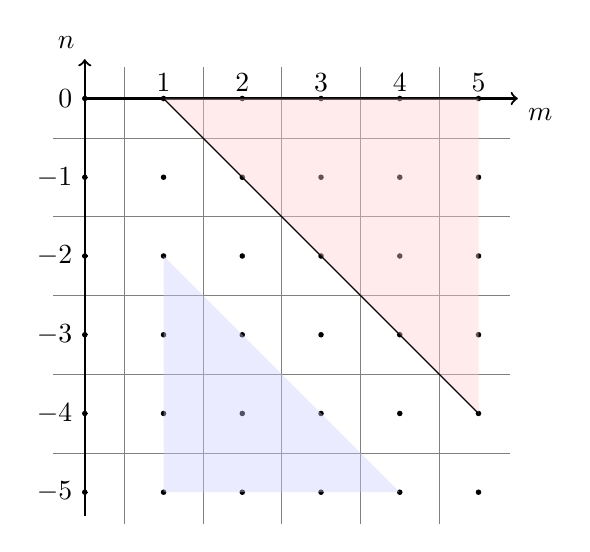
\begin{tikzpicture}
    \draw[step=1cm,gray,very thin, xshift=0.5cm, yshift=-0.5cm] (-0.9,0.9) grid (4.9,-4.9);
    \draw[thick,->] (0,0) -- (5.5,0) node[anchor=north west] {\( m \)};
    \draw[thick,->] (0,-5.3) -- (0,0.5) node[anchor=south east] {\( n \)};
    \foreach \x in {1,2,3,4,5}
    \draw (\x cm,1pt) -- (\x cm,-1pt) node[anchor=south] {$\x$};
    \foreach \y in {0, -1,-2,-3,-4,-5}
    \draw (1pt,\y cm) -- (-1pt,\y cm) node[anchor=east] {$\y$};

    \foreach\x in {0,...,5} {
      \foreach \y in {0,-1,-2,-3,-4,-5} {
        \fill (\x, \y) circle[radius=1pt];
      }
    }
    % \fill[blue!20, opacity=0.4] (-0.5, 0) -- (4, -4.5) -- (-0.5, -4.5) -- (-0.5, 0);
    % \fill[red!20, opacity=0.4] (0, -0.5) -- (4.5, -5) -- (4.5, -0.5) -- (0, -0.5);
    \fill[red!20, opacity=0.4] (1, 0) -- (5, -4) -- (5, 0) -- (1, 0);
    % \fill[blue!20, opacity=0.4] (1,0) -- (5, -4) -- (1, -4) -- (1,-1);
    \fill[blue!20, opacity=0.4] (1,-2) -- (4, -5) -- (1, -5) -- (1,-2);
    \draw (1, 0) -- (5, -4);
  \end{tikzpicture}
  \caption{The region of \( (m,n) \) to sum over for a Type-I perpendicularly tilted cone.
    The black line represents the combinations that give a finite contribution also in the untilted case.
    As the cone is tilted, this sharp line ``diffuse'' into the red and blue regions as well, where the contribution is respectively positive and negative.
    Note that, as \( \Xi_1 \) defined only for \( M>0\), the region with \( m=0 \) gives no contribution;
    at \( M=N \) the contribution is also zero.%
  }
  \label{fig:nmregion}
\end{figure}

\begin{figure}[htb]
  \centering
  \pgfplotsset{
  % colormap={X}{ gray(0cm)=(1); gray(1cm)=(0);},
  % colormap={mycool}{ rgb255(0)=(255,0,255); rgb255(8)=(0,128,255); rgb255(10)=(255,255,255);},
  colormap={temp}{rgb255=(36,0,217) rgb255=(25,29,247) rgb255=(41,87,255)
    rgb255=(61,135,255) rgb255=(87,176,255) rgb255=(117,211,255)
    % rgb255=(153,235,255)
    rgb255=(255,255,255)
    % rgb255=(255,214,153)
    rgb255=(255,172,117) rgb255=(255,120,87) rgb255=(255,61,61)
    rgb255=(247,40,54) rgb255=(217,22,48) rgb255=(166,0,33)},
  % colormap={mycool}{ rgb255(-1)=(255,0,255); rgb255(-0.1)=(255,0,255); rgb255(0)=(255,255,255); rgb255(1)=(0,128,255)},
  % colormap={violet}{rgb255=(25,25,122) color=(white) rgb255=(238,140,238)},
  point meta min=-0.1,
  point meta max=0.1,
  xlabel=\( m \),
  ylabel=\( n \),
}
\newcounter{plotnum}
\tikzsetnextfilename{contribmn-P}
\begin{tikzpicture}
  \begin{groupplot}[
    width=0.5\textwidth,
    unit vector ratio=1 1 1,unit rescale keep size=false, %% Do not enlarge limit, keep unit equal
    xmin=-6.5, xmax=6.5,
    ymin=-6.5, ymax=6.5,
    % title={\( t_x= \title \)},
    title style={ at={(0.75, 0.7)} },
    group style={
      group size=2 by 2,
      group name=contribs,
      x descriptions at=edge bottom,
      y descriptions at=edge left,
      horizontal sep=8pt,
      vertical sep=8pt,
    },
    ]
    \pgfplotsforeachungrouped \datafile/\title in {
      contribTilttx0.PbrokenFalse.csv/0,
      contribTilttx0.125PbrokenFalse.csv/0.16,
      contribTilttx0.25PbrokenFalse.csv/0.25,
      contribTilttx0.5PbrokenFalse.csv/0.5
    }{
      \edef\tmp{
        \noexpand\ifthenelse{\theplotnum=1}{
          \noexpand\nextgroupplot[title={$t_x = \title$}, colorbar right,
          every colorbar/.append style={height=
            2*\noexpand\pgfkeysvalueof{/pgfplots/parent axis height}+8pt, ytick={-0.1,0,0.1}},
          colorbar to name={mycolorbar}
          ]
          % See  https://tex.stackexchange.com/questions/126177/common-colorbar-for-groupplot
        }{
          \noexpand\nextgroupplot[title={$t_x = \title$}]
        }
        % \noexpand\nextgroupplot[title={$t_x = \title$}, colorbar, colorbar horizontal, colorbar to name={mycolorbar}]
        \noexpand\addplot [
        matrix plot*,
        mesh/cols=13,
        point meta=explicit,
        ] table[x=m, y=n, meta=Contrib, col sep=comma] {data/\datafile};
      }
      \tmp

      \ifthenelse{\theplotnum=0}{
        \draw[dotted, gray] (axis cs:-1.5,-1.5) rectangle (axis cs:1.5,1.5) node[pos=0, pin={[pin edge={solid}]-180:\( \gamma_0 \)}] {};
        \draw[dotted, gray] (axis cs:-2.5,-2.5) rectangle (axis cs:2.5,2.5) node[pos=0, pin={[pin edge={solid}]-110:\( \gamma_1 \)}] {};

        % \draw[dotted, gray] (axis cs:0.5,-0.5) rectangle (axis cs:1.5,0.5) node[pos=0, yshift=4pt, pin={[pin edge={solid}]-140:\( \gamma_0 \)}] {};
        % \draw[dotted, gray] (axis cs:0.5,-1.5) rectangle (axis cs:2.5,0.5) node[pos=0, pin={[pin edge={solid}]-140:\( \gamma_1 \)}] {};
        % \draw[dotted, gray] (axis cs:0.5,-3.5) rectangle (axis cs:4.5,0.5) node[pos=0, pin={[pin edge={solid}]-140:\( \gamma_3 \)}] {};
      }{}
      \stepcounter{plotnum}
    }
  \end{groupplot}
  %% Shfit half vertical sep
  \node[anchor=west, yshift=4pt] at (contribs c2r2.north east) {\ref{mycolorbar}};
\end{tikzpicture}

  \caption{Contributions to \( \gamma_N \) from \( m\to n \) transitions for different values of \( t_x \).
    In order to retain contrast, the color values are capped at \( 0.1 \), meaning that the \( \gamma_0 \) contributions are clipped.
    Note that all quadrants of the \( m,n \)-plane are shown, although as proven in the main text, only the fourth quadrant needs to be computed, as the second quadrant contributions are equal.
    Lastly, the \( \gamma_N \) square regions indicated in the first pane are drawn with lengths \( 2N + 1 \), while they in the main text are defined with sides \( 2N \);
    this choice of representation is only to make the figure more clear, as the colored tiles have edges at half-integer values.
    \label{fig:contribs}
    }
\end{figure}

\subsection{Tilt parallell to the magnetic field}
Even though the treatment above for a general tilt is valid for parallel tilt, the response can be found more directly from the untilted case.
For \( \vec{t} = t_z \hat{z} \), the energy momentum tensor \( T^{y 0} \), charge current \( J^x \), and wave functions \( \phi(\vec{r}) \) are all independent of \( t_z \), and the only difference compared to the untilted system is a change in the energies of the Landau levels.
We may thus immediately use the result from the untilted case
\begin{multline}
  \label{eq:120}
  \lim_{\omega \to 0} \lim_{\vec{q} \to 0} \chi^{xy} =
  - \frac{e^2 v_F B}{2 (2\pi)^2}
  \sum\limits_{mn} \int \mathrm{d} \kappa_z
  \xi(\kappa_z)
  (\epsilon_{\kappa_z m s} + \epsilon_{\kappa_z n s})\\
  \times (\alpha_{\kappa_z m s}^2 \delta_{M-1, N} - \alpha_{\kappa_z n s}^2 \delta_{N-1, M}),
\end{multline}
with
\begin{align}
  \label{eq:121}
  \epsilon_{\kappa_z m s} &=
                          \begin{cases}
                            t_z^s \kappa_z + \sign{m} \sqrt{M + \kappa_z^2} & m \neq 0,\\
                            (t_z^s - s) \kappa_z & m = 0,
                          \end{cases}\\
  \alpha_{\kappa_z m s} &=
                          -s \frac{\sqrt{M}}{\epsilon_{\kappa_z  m s}^0 - s \kappa_z },\\
  \lim_{\omega \to 0} \lim_{\vec{q} \to 0}\xi(\kappa_z) &= \frac{[n_{\kappa ms} - n_{\kappa ns}]
  \left[ (\alpha_{\kappa ms}^2 + 1) (\alpha_{\kappa ns}^2 + 1) \right]^{-1}
  }{
    (\epsilon _{\kappa m s} - \epsilon _{\kappa n s})^2
  }.
\end{align}
In the untilted case we made several simplifications to this expression, especially with regard to limiting the summation domain.
We will here consider which of those simplifications apply also in the case of tilt \( t_z \).

Under the transformation \( (m,n,\kappa_z) \mapsto (-m, -n , -\kappa_z) \), \( \xi(\kappa_z), \epsilon_{\kappa_z m s}, \alpha_{\kappa_z m s} \) are all still odd, and so the integrand is invariant under such a transformation.
As the integral is over all \( \kappa_z \), we may therefore consider only half the \( m,n \) plane, as was the case in the untilted case.
However, in the untilted case the sum was in fact restricted to only one quadrant, as at \( T\to 0 \) the transitions must be between states with energy of opposite sign.
In the case of Type-II systems, this requirement does not restrict the sum to one quadrant.
It is thus convenient to consider Type-I and Type-II separately.

In the untitled system, the contributions from the two chiralities where the same, as \( \kappa_z \) and \( s \) always appeared in conjunction, \( \kappa_z s \).
In the case of \( t_z \) tilt, this is not the case.
The proof for the response from the two chiralities being the same in the untilted case was that \( s \) and \( \kappa_z \) appeared only through the product \( s \kappa_z \), and so the expression was invariant under \( (s, \kappa_z) \mapsto (-s, -\kappa_z) \).
As our integration spans all \( \kappa_z \), the total response is invariant under \( s \to -s \).
The tilt parameter enters the expression only through \( \epsilon_{\kappa_z m s} = \epsilon_{\kappa_z m s}^0 + \kappa_z t^s_z \), and in the inversion symmetric case, \( t^s_z = s t_z \), the argument still holds.
In the case of broken inversion symmetry, however, where \( t^s_z = t_z \), the argument fails.
A similar argument may, however, be made for the transformation \( (s, \kappa_z, t_z) \mapsto (-s, -\kappa_z, -t_z) \), for which the (inversion broken) system is invariant.
The response of a cone with chirality \( s = -1 \) is thus equal the response with \( s = +1 \) and \( t_z \to -t_z \).
We therefore compute all responses for \( s=+1 \);
for symmetric systems the response is equal for \( s=-1 \), while for broken inversion symmetry, the response is given at \( t_z \to -t_z \).

\subsubsection{Type-I}
In Type-I systems, the selection rules from the step functions are independent of \( t_z \), and the only difference from the untilted case is the term \( \epsilon_{\kappa_z m s} + \epsilon_{\kappa_z n s} = \epsilon^0_{\kappa_z m s} + \epsilon^0_{\kappa_z n s} + 2 \kappa_z t^s_z \).
The response is therefore
\begin{equation}
  \label{eq:122}
  \lim_{\omega \to 0} \lim_{\vec{q} \to 0} \chi^{xy} = \frac{e^2v_F B}{2 (2\pi)^2} (\gamma_N^0 + \gamma_{\text{div}, N}),
\end{equation}
where \( \gamma_N^0 \) is the prefactor of the untilted case, and according to Eq.~\eqref{eq:93}
\begin{equation}
  \label{eq:123}
  \gamma_{\text{div}, N} = -4 \sum\limits_{i=0}^{N} \int \mathrm{d} \kappa_z \xi(\kappa_z)
  2 \kappa_z t^s_z \alpha_{\kappa_z m s}^2 \Big|_{\overset{m=i+1}{n=-i}},
\end{equation}
which has an UV divergence.
Introduce the momentum cutoff \( \Lambda \), in which case the integral can be solved analytically, with the result\footnote{Note the minus sign introduced by the step function in \( \xi \).}
\begin{equation}
  \label{eq:124}
  \gamma_{\text{div}, 0} = 2 t_z \left(\Lambda  \left(\Lambda -\sqrt{\Lambda ^2+1}\right)+\sinh ^{-1}(\Lambda
   )\right)
\end{equation}
and the contribution from each term of the sum
\begin{multline}
  \gamma_{\text{div}, N} - \gamma_{\text{div}, N-1} =
  2 t_z
  \Bigg\{
    \Lambda\left(\sqrt{\Lambda^2 + N} - \sqrt{\Lambda^2 + N + 1}  \right)\\
    + (N + 1) \tanh^{-1}\left[\frac{\Lambda}{\sqrt{\Lambda^2 + N + 1} } \right]
    - N \tanh^{-1}\left[\frac{\Lambda}{\sqrt{\Lambda^2 + N}}\right]
    \Bigg\},
    \label{eq:125}
\end{multline}
where we used the selection rule of the sum \( N = M - 1 \) and \( m>0, n<0 \).
This contribution is shown in figure \ref{fig:divergent-factor}.
\todo{is it ok to write 'the contribution \eqref{eq:125}', or must it always be 'the contribution Eq. \eqref{eq:125}'?}
The contribution \eqref{eq:125} is odd in \( t_z \), and so for systems with broken inversion symmetry, the total contribution from two cones cancel.

Assuming \( \Lambda \gg 1 \) the expression is approximated by
\begin{equation}
  \label{eq:126}
  t_z
  \left(
    \left[
  -1 + N \log\left(\frac{N}{N+1}\right) - \log \frac{N+1}{4}
  \right]
 + 2 \log\Lambda
\right) + \mathcal{O}\left(\frac{1}{\Lambda^2}\right).
\end{equation}
The contribution is shown in figure~\ref{fig:divergent-factor} for the first Landau levels.



\subsubsection{Type-II}
For Type-I semimetals, the sign of energy state \( m \neq 0 \) is given by the sign of \( m \) itself.
For \( m = 0 \) the sign of the energy is given by \( -s \sign{\kappa } \).
Due to this, the sum is restricted to \( n=M+1, m=-M \) and \( n=-M-1, m=M \).
In the case of Type-II, however, the situation is not so simple.
The energy bands cross the Fermi surface, and we must also include in our sum overlap between states of the same sign, i.e. \( n=M+1, m=M \) and \( n=-M-1, m=-M \), which is non-zero for certain intervals of \( \kappa  \).
See plot of the tilted Landau levels in figure~\ref{fig:llevelstilt}.

% Furthermore, the expression is no longer invariant under \( (s, \kappa_z) \mapsto (-s, -\kappa_z) \).
% For inversion symmetric systems, \( \vec{t^s} = s \vec{t} \), the symmetry is still conserved, however, for broken inversion symmetry, the extra term in the energies, \( t^s_z \kappa_z \) breaks the symmetry between the chiralitites.
% As the energies change between the chiralities, so does the step function, giving other selection rules.
% For inversion symmetric systems, we may thus simply choose a value of \( s \), for example \( s=1 \), and compute all results for that value.
% For broken inversion symmetry, however, the results must be computed separately for the two chiralities.
% \todo{Or maybe it is easier to do all calculations with \( t_x^s \) (and its sign) in focus, and then later apply inversion (broken) symmetry?}

In order to find explicitly the limits of integration for the Type-II case, we must find the roots of the energy levels.
The zeroth Landau level always has only one root, which is in the origin.
For the higher order Landau levels, we solve
\begin{equation}
  \label{eq:127}
  \epsilon_{\kappa_z m s } = t_z^s \kappa_z + \sign(m) \sqrt{M + \kappa_{z} ^2} = 0,
\end{equation}
whose solution is
\[
\kappa_z^2 = \frac{M}{t_{z}^2 - 1}.
\]
The actual roots of the energies are
\begin{equation}
  \label{eq:128}
  \kappa_z = -\sign(m t^s_x) \sqrt{\frac{M}{t_{z}^2 - 1}}.
\end{equation}
The integration limit for the \( 0 \to 1 \) transition is thus, for \( t_z > 1 \), \( [-\sqrt{t_z^2 - 1 }^{-1}, 0] \).
The \( 1\to 2 \) transition is \( [-\sqrt{2} /\sqrt{t_z^2 - 1}, -\sqrt{t_z^2 - 1 }^{-1}] \), and so forth.
The general \( n \to m \) transition has the integration limits
\[
  \left[-\sign(t_z) \sqrt{\frac{m}{t_{z}^2 - 1}}, -\sign(t_z n) \sqrt{\frac{-n}{t_{z}^2 -1}} \right].
\]

The \( 0\to 1 \) transitions was computed analytically, and found to be
\begin{equation}
  \label{eq:129}
  \gamma_0 =
  2 \sign(t_z)
  \left(
  |t_z| \sinh^{-1}\left(\frac{1}{\sqrt{t_{z}^2-1} }\right) -1
\right  ).
\end{equation}
For a general \( n \to m, \; N>0, M=N+1 \) transition, the contribution \( \gamma_N - \gamma_{N-1} \) was found to have very lengthy expressions.
Consult Table~\ref{tab:typeii-expressions} to find the appropriate expressions for positive and negative tilt, and interband and intraband transitions.

\begin{table}[ht]
  \centering
  \renewcommand\arraystretch{2.5}
  \begin{tabular}{ll | c | c |}
    &\multicolumn{1}{c}{}&\multicolumn{2}{c}{\textbf{Tilt direction}}\\[-2ex]
    &\multicolumn{1}{c}{}
                         &\multicolumn{1}{c}{\( t_x > 1 \)}&\multicolumn{1}{c}{\( t_x < -1 \)}\\
    \cline{3-4}
    \multirow{2}{*}{\rotatebox{90}{\textbf{Band type}}}
    &\( n < 0 \)& Lst.~\ref{lst:typeii-interband-tzpos} & Lst.~\ref{lst:typeii-interband-tzneg}\\
    \cline{3-4}
    &\( n > 0 \)& Lst.~\ref{lst:typeii-intraband-tzpos} & Lst.~\ref{lst:typeii-intraband-tzneg}\\
    \cline{3-4}
  \end{tabular}

  % \begin{tabular}{l | c | c |}
  %   \multicolumn{1}{c}{}
  %                        &\multicolumn{1}{c}{\( t_x > 1 \)}&\multicolumn{1}{c}{\( t_x < -1 \)}\\
  %   \cline{2-3}
  %   \( n < 0 \)& Lst.~\ref{lst:typeii-interband-tzpos} & Lst.~\ref{lst:typeii-interband-tzneg}\\
  %   \cline{2-3}
  %   \( n > 0 \)& Lst.~\ref{lst:typeii-intraband-tzpos} & Lst.~\ref{lst:typeii-intraband-tzneg}\\
  %   \cline{2-3}
  % \end{tabular}

  \caption{
    % The expression for the \( m\to n; N> 0, M=N+1 \) transition is given by the equation number at the various choices of \( t_z \) and \( \sign (n) \).
    Decision matrix for the expression of the \( m \to n; N > 0, M =N+1 \) transition over different regions.
    Expressions given in Mathematica code format;
    the code listings are found in \cref{cha:long_expression}.
    % Code listings starting on page \pageref{lst:typeii-interband-tzpos} in \cref{cha:long_expression}.
    See main text for details.%
  }
  \label{tab:typeii-expressions}
\end{table}


\FloatBarrier
\section{Results}
In the static and local limit $\lim_{\omega \to 0} \lim_{\vec{q}\to 0}$ the  transverse response function $\chi^{xy}$ of the charge current to a temperature perturbation
\begin{equation}
  J^x = \chi^{xy} \frac{- \nabla^y T}{T}
\end{equation}
from a single Weyl cone was found  to be
\begin{equation}
  \lim_{\omega \to 0} \lim_{\vec{q}\to 0}
  \chi^{xy}
  =
  \gamma_{N}
  \frac{e^2 B v_F}{2 (2\pi )^2 \hbar },
\end{equation}
with $\gamma _N$ a prefactor dependent on the chirality \( s \), the tilt \( \vec{t} \), and  how many landau levels are included in the final evaluation of the response function.

In general, the prefactor \( \gamma_N \) diverges as $N\to \infty$.
However, not all Landau levels are filled, and thus the sum should not be taken to all levels.
Similarly to a quantum Hall effect, the number of filled bands, the filling factor $\nu $, is inverse proportional to the $B$-field strength
\begin{equation}
  \nu \propto \frac{1}{B}.
\end{equation}
Thus, we expect that the $N$-sum should be truncated at a Landau level, given by the filling factor $\nu $.
A detailed derivation of the exact truncation of the $N$-sum has not been done.
If a precise result for the numerical prefactor is found to be of importance, this should be straightforward.

As described above, the contribution from the cone with chirality \( s = -1 \) can be found from the result of the positive chirality cone.
In the case of perpendicular tilt, they are exactly the same.
In the case of parallel tilt, it depends on the symmetry of the tilt.
For systems with inversion symmetry, the responses from the two cones are the same.
On the other hand, for broken inversion symmetry, the contribution from the cone with chirality \( s=-1 \) is the same as that of the \( s=+1 \) cone at the opposite tilt \( t_z \to - t_z \).
Therefore, it is useful to separate the contribution into even and odd components, for finding the total contribution from the two cones combined.
Separating even and odd components also alows for presenting the data in more compact plots.

For some contribution \( \gamma(t_{x /z}) \), we define
\begin{align}
  \gamma_{\text{even}}(t_{x/z}) &= \frac{\gamma(t_{x/z}) + \gamma(-t_{x/z})}{2}\label{eq:130},\\
  \gamma_{\text{odd}}(t_{x/z}) &= \frac{\gamma(t_{x/z}) - \gamma(-t_{x/z})}{2}\label{eq:131}.
\end{align}
All results will be given in terms of these components, at \( t_{x /y} > 0 \).
The total contribution \( \gamma_{\text{tot}} \) for the two cones is found by taking the appropriate combinations of \cref{eq:130,eq:131}, as shown in \cref{tab:gamma-tot}.

\begin{table}[h]
  \centering
  \begin{tabular}{l c}
    \toprule
    Case & Total contribution, \( \gamma_{\text{tot}} /2 \)\\
    \midrule
    Perpendicular tilt & \( \gamma_{\text{even}} + \gamma_{\text{odd}} = \gamma \)\\
    Parallel tilt, broken inversion symmetry & \( \gamma_{\text{even}} \)\\
    Parallel tilt, inversion symmetry &  \(  \gamma_{\text{odd}} + \gamma_{\text{even}} = \gamma \)\\\bottomrule
  \end{tabular}
  \caption{The total contribution from two cones \( \gamma_{\text{tot}} \) is found by linear combinations of the even and odd components of \( \gamma \), depending on the case at hand.
    Note that total contribution given in the table is \( \gamma_{\text{tot}} /2 \).
    \label{tab:gamma-tot}}
\end{table}

\subsection{Perpendicular tilt}
In the case of a tilt perpendicular to the magnetic field, we are, as previously explained, restricted to Type-I materials, as the Landau level description breaks down for Type-II perpendicular tilt.
Importantly, this does not generally mean that the effect is not present for Type-II systems, but simply that the linear model Landau level description is not a good basis for the system.
The collapse of the Landau levels caused \textcite{soluyanovTypeIIWeylSemimetals2015} to erroneously predict the collapse of the chiral anomaly in their now famous paper first describing Type-II Weyl semimetals.

As explained in section \ref{sec:perptiltsum}, the \( m,n \) summation is restricted to the fourth quadrant in the \( m,n \) plane.
In the case of no tilt, only contributions from \( M = N + 1 \) were non-zero;
we named the contribution from the \( 0\to 1 \) transition \( \gamma_0 \), the \( -1\to 2 \) transition \( \gamma_1 \) and so forth.
For perpendicular tilt, as there are contributions also away from the \( M=N + 1 \) line, we denote by \( \gamma_0 \) the contributions from inside the square of length 2 centered at the origin.
The \( \gamma_1 \) contributions are those inside the square of length 4, and in general \( \gamma_n \) the square with length \( 2 n \).
This is indicated in figure~\ref{fig:contribs}.
This definition effectively sets a ceiling on which Landau levels we consider.

\todo{Correct which values }
The integral was computed numerically for \( M,N \leq 6 \) over different values of \( t_x \) with \( t_z = 0 \), with the individual contributions shown in figure~\ref{fig:contribs}.
Note that the figure shows contributions for the entire \( m,n \)-plane, not only the fourth quadrant as discussed above.
This is purely for illustration purposes, and only the fourth quadrant needs to be computed.
The total contribution \( \gamma_N \) as a function of \( N \) is shown in figure~\ref{fig:total_contribs}.
The contribution is even in \( t_x \), and the two cones have the same contribution, as shown analytically in section~\ref{sec:perptiltsum}.
Also shown in figure~\ref{fig:total_contribs} is \( \gamma_0 \) as a function of \( t_x \), which is seen to be strictly decreasing to zero as \( t_x \to 1 \).
This last observation is discussed further in section~\ref{sec:other-observe:zeroton}, under
``\nameref{sec:other-observe:zeroton}''.

\begin{figure}[ht]
  \centering
  \tikzsetnextfilename{contribtx}
  \resizebox{0.8\textwidth}{!}{
  \begin{tikzpicture}
    \pgfplotsset{set layers} %% See 4.9.11 in PGFPlots manual
    \begin{axis}[
      axis x line*=top, axis y line*=right,
      scale only axis,
      width=12cm,
      height=8cm,
      tick label style={gray},
      ylabel=\( \gamma_0(t_x) \),
      xlabel=\( t_x \),
      x label style={at={(axis description cs:0.95,1.02)}, anchor=south west, gray},
      y label style={gray},
      ]
      \addplot[teal!60, dashed] table[col sep=comma] {data/contribTilttx-zerothll.csv};
    \end{axis}
    \begin{axis}[
      legend columns=-1,
      legend style={at={(0.5, 1.1)}, anchor=south,},
      % legend to name=contribs,
      xlabel=Number of Landau levels,
      ylabel=\( \gamma_N \),
      width=12cm,
      height=8cm,
      name=myaxis,
      axis x line*=bottom, axis y line*=left,
      xtick distance=1,
      scale only axis,
      ]
      \newcommand\plotContrib[1]{
        % \addplot table[col sep=comma] {data/contribSumTilttx#1PbrokenTrue.csv};
        \addplot table[y=#1, col sep=comma] {data/contribSumTilttx.csv};
        % \addlegendentry{\( t_x = \num[minimum-decimal-digits=3]{#1} \)}  %% Make all same length
        \addlegendentry{\( t_x = \num[minimum-decimal-digits=1]{#1} \)}
      }
      \plotContrib{0.}
      \plotContrib{0.125}
      \plotContrib{0.25}
      \plotContrib{0.375}
      \plotContrib{0.5}
      % \plotContrib{0.625}
      % \plotContrib{0.75}
      % \plotContrib{0.875}
      % \plotContrib{0.99}

      % \addplot table[col sep=comma] {data/contribSumTilttx0.PbrokenTrue.csv};
      % \addplot table[col sep=comma] {data/contribSumTilttx-0.PbrokenTrue.csv};
      % \addplot table[col sep=comma] {data/contribSumTilttx-0.125PbrokenTrue.csv};
      % \addplot table[col sep=comma] {data/contribSumTilttx-0.25PbrokenTrue.csv};
      % \addplot table[col sep=comma] {data/contribSumTilttx-0.375PbrokenTrue.csv};
      % \addplot table[col sep=comma] {data/contribSumTilttx-0.5PbrokenTrue.csv};
    \end{axis}
    % \node[anchor=south] at (myaxis.north) {\ref{contribs}};
  \end{tikzpicture}
  } %% Resizebox
  \caption{Total contribution \( \gamma_N \) for a perpendicular tilt \( t_x \), which only has an even component.
    See main text for details on how \( \gamma_N \) is defined.
    Shown in dashed \textcolor{teal!80!black}{teal} on secondary axis (gray labels) is \( \gamma_0 \) as a function of \( t_x \), which is strictly decreasing from 1 at \( t_x = 0 \) to 0 at \( t_x = 1 \).
    \label{fig:total_contribs}}
\end{figure}

\FloatBarrier
\subsection{Parallel tilt}
\subsubsection{Type-I}
\todo{Should we also compute the momentum cutoff for nontilted terms?}
In the Type-I regime, the contributions differ from that of the untitled system by \( \gamma_{\text{div}, N} \), Eq. \eqref{eq:123}, dependent on a momentum cutoff \( \Lambda = k^{\text{cutoff}} /\sqrt{2 e B}  \), where \(k^{\text{cutoff}}\) is the physical cutoff.
In the large cutoff limit, \( \Lambda \gg 1 \), expanding and dropping terms \( \mathcal{O}(1 /\Lambda^2) \), we found Eq.~\eqref{eq:126},
\[
  \gamma_{\text{div}, N} - \gamma_{\text{div}, N-1} =
  t_z
  \left(
    \left[
      -1 + N \log\left(\frac{N}{N+1}\right) - \log \frac{N+1}{4}
    \right]
    + 2 \log\Lambda
  \right).
\]
The first term, independent of \( \Lambda \), is a negative factor that decreases as \( N \) increases, and goes like \( -\log N \) for large \( N \).
The contribution is proportional to \( t_z \), i.e. there is no even component, so for systems with broken inversion symmetry, the two chiralities cancel, and the response is equal to the untilted case.
In the case of inversion symmetry, the contributions from the two chiralities are equal and add up.
The contribution has the same sign as the tilt, and the magnitude depends on the landau cutoff \( N \) and momentum cutoff \( \Lambda \).


\begin{figure}[htp]
  \centering
  \tikzsetnextfilename{divergentContribCutoff}
    \begin{tikzpicture}
      \begin{axis}[
        xlabel=\( \Lambda \),
        ylabel={\( [ \gamma_{\text{div}, N} - \gamma_{\text{div}, N-1}] /t_z \)},
        legend pos=south east,
        % cycle list name=exotic,
        cycle list={
          teal,every mark/.append style={fill=teal!80!black},mark=*\\
          orange, dashed, every mark/.append style={fill=orange!80!black},mark=square*\\
          cyan!60!black, densely dotted, every mark/.append style={fill=cyan!80!black},mark=otimes*\\
          red!70!white, dashdotted, mark=star\\
          lime!80!black, loosely  dashed, every mark/.append style={fill=lime},mark=diamond*\\
          red,densely dashed,every mark/.append style={solid,fill=red!80!black},mark=*\\
          yellow!60!black,densely dashed,
          every mark/.append style={solid,fill=yellow!80!black},mark=square*\\
          black,every mark/.append style={solid,fill=gray},mark=otimes*\\
          blue,densely dashed,mark=star,every mark/.append style=solid\\
          red,densely dashed,every mark/.append style={solid,fill=red!80!black},mark=diamond*\\
        },  %% exotic with various line types
        ]
        \foreach \i in {1,...,5} {
          \addplot+[mark=none] table[x index=0, y index=\i, col sep=comma] {data/divergentFactor.csv};
          \addlegendentryexpanded{\( N = \the\numexpr\i-1\relax \)};
        }
      \end{axis}
    \end{tikzpicture}
    \caption{The divergent factor \( \gamma_{\text{div}, N} / t_{z} \) for the first Landau levels, as a function of the momentum cutoff \( \Lambda \).
    \label{fig:divergent-factor}}
\end{figure}

\FloatBarrier
\subsubsection{Type-II}
In the Type-II regime, the contributions have a more complicated form.
Considering firstly only the lowest Landau level contribution, Eq.~\eqref{eq:129}, which is odd in \( t_z \), the total contribution cancels between the chiralities for broken inversion symmetry, while it adds up for inversion symmetric systems.
As \( |t_z| \to 1 \) from above, the contribution blows up.
This is to be expected as we move towards the Lifshitz transition, where we expect the linear model to perform poorly.\footnote{As the Fermi surface of the linear model is vastly different from the Fermi surface of the tight binding model.
See discussion on page \pageref{sec:tilt:fermisurface-paragraph} in section \ref{sec:tilt:fermisurface-paragraph} and  \textcite{vanderwurffMagnetovorticalThermoelectricTransport2019}.}
The contribution goes to zero as \( t_z \to \infty \), shown in \cref{fig:contribtzII}.

Considering also higher Landau level contributions, both interband and intraband transitions must be included,%
\footnote{By band we here refer to the ``conduction'' band and ``valence'' band.}
meaning the summation is no longer restricted to a quadrant in the \( m,n \) plane, but rather to half the plane.
The contributions are shown in figure \ref{fig:contribtzII}.
These contributions are not odd in \( t_z \) -- they have a finite even component.
Due to this, the contribution does not cancel for inversion broken systems, however, the even contribution is small in magnitude compared to the other contributions.

A schematic plot of all the contributions of a parallel tilt is shown in \cref{fig:scetch}.
In systems with broken inversion symmetry, where only the even contribution survives, we see that in the Type-I regime, the response is independent of the tilt \( t_z \).
In the Type-II regime, the response has the opposite sign, and is heavily reduced in magnitude;
for a sufficiently large magnetic field, when only the zeroth Landau level is filled, the effect is non-existent.

\begin{figure}[ht]
  \centering
  \subcaptionbox{Intraband contributions, \( -N \to N + 1 \).}{
  \tikzsetnextfilename{tzcontribtypeii}
  \begin{tikzpicture}
    \pgfkeys{/pgf/declare function={arcsinh(\x) = ln(x + sqrt(x^2+1));}}
    \begin{axis}[
      width=0.49\textwidth,
      domain=1:2,
      xlabel=\( t_z \),
      ylabel={Contribution \( \gamma \)},
      samples=100,
      legend entries={%
        \( \hphantom{-}0\rightarrow 1\),
        \( -1 \rightarrow 2\),
        \( -2\rightarrow 3 \),
        \( -3\rightarrow 4 \),
      }, %% There is a bug with \to
      % cycle list={[samples of colormap={4} of colormap/autumn]},
      % cycle list={[of colormap=colormap/autumn]},
      ]
      % \addplot[mark=none] {0.5 * (x * arcsinh(1/sqrt(x^2-1)) - 1)};
      % \addplot+[mark=none] {(-1 + x * ln((1+x)/sqrt(x^2-1)))}; %% Same as above, just more stable
      \addplot+[mark=none] table[col sep=comma, y=1] {data/contribtypeii_interband_odd.csv};
      \addplot+[mark=none] table[col sep=comma, y=2] {data/contribtypeii_interband_odd.csv};
      \addplot+[mark=none] table[col sep=comma, y=3] {data/contribtypeii_interband_odd.csv};
      \addplot+[mark=none] table[col sep=comma, y=4] {data/contribtypeii_interband_odd.csv};

      \pgfplotsset{cycle list shift=-3}  %% Change shift to number of transitions > 0
      \addplot+[mark=none, dashed] table[col sep=comma, y=2] {data/contribtypeii_interband_even.csv};
      \addplot+[mark=none, dashed] table[col sep=comma, y=3] {data/contribtypeii_interband_even.csv};
      \addplot+[mark=none, dashed] table[col sep=comma, y=4] {data/contribtypeii_interband_even.csv};
    \end{axis}
  \end{tikzpicture}
  } %% Subcaptionbox
  \subcaptionbox{Interband contributions, \( N \to N + 1 \).}{
  \tikzsetnextfilename{tzcontribtypeii_intraband}
  \begin{tikzpicture}
    \begin{axis}[
      width=0.49\textwidth,
      domain=1:2,
      xlabel=\( t_z \),
      % ylabel=Contribution,  %% Enough with one
      legend entries={%
        \( 1 \rightarrow 2\),
        \( 2\rightarrow 3 \),
      }, %% There is a bug with \to
      ]
      % \addplot[mark=none] {0.5 * (x * arcsinh(1/sqrt(x^2-1)) - 1)};
      \addplot+[mark=none] table[col sep=comma, y=2] {data/contribtypeii_intraband_odd.csv};
      \addplot+[mark=none] table[col sep=comma, y=3] {data/contribtypeii_intraband_odd.csv};

      \pgfplotsset{cycle list shift=-2}
      \addplot+[mark=none, dashed] table[col sep=comma, y=2] {data/contribtypeii_intraband_even.csv};
      \addplot+[mark=none, dashed] table[col sep=comma, y=3] {data/contribtypeii_intraband_even.csv};
    \end{axis}
  \end{tikzpicture}
  } %% subcaptionbox
  \caption{The contribution from \( n\to m \) transitions in a Type-II \(t_z\) tilted system.
    Solid line is the odd component \( \gamma_{\text{odd}} \), dashed is even component \( \gamma_{\text{even}} \).
    % Shown in dashed line is the difference between the contribution at \( t_z \) positive and negative.
  }
  \label{fig:contribtzII}
\end{figure}

\begin{figure}[p]
  \centering
  \tikzsetnextfilename{schematic_tz}
  \begin{tikzpicture}
    \begin{axis}[
      ymax=1,
      xmin=0, xmax=2,
      width=13cm, height=10cm,
      legend entries={Even,Odd},
      xtick={0,1,2},
      ytick=\empty,
      xlabel=\( t_z \),
      ]
      \draw[thin, gray, dashed](axis cs:1,-1)--(axis cs:1,1.2);
      \addplot[forget plot, thin] {0};

      \addplot[mark=none, domain=0:1] {0.5} node[midway, pin=above:Untilted contribution] {};
      \addplot[mark=none, dashed, domain=0:1] {0.2 * x} node[midway, pin={[pin edge=solid]above:\( \propto \log\Lambda \)}] {};
      \addplot[dashed, mark=none] table[col sep=comma, y=-1] {data/contribtypeii.csv};
      \addplot[mark=none] table[col sep=comma, y=-1] {data/contribtypeii_diffsigntz.csv};
    \end{axis}
  \end{tikzpicture}
  \caption{
    Schematic summary of the contribution for parallel tilt \( t_z \).
    Shown is the even (solid line) and odd (dashed line) parts as a function of \( t_z \).
    As explained in the main text and shown in \cref{tab:gamma-tot}, the total contribution for a pair of cones is given by the sum of the components in inversion symmetric systems, and by the even component for broken inversion symmetric systems.
    Note that, as the contributions depend on factors such as the number of Landau levels and momentum cutoff, their relative magnitudes in the sketch are of little importance.
    \label{fig:scetch}
  }
\end{figure}

\FloatBarrier
\subsection{Other observations}\label{sec:other-observe}
We here present some further observations that are of interest, which we have been unable to investigate further due to time constraints.
We therefore do not have conclusive result, and do not want to present them together with the main results.
However, they are of great importance, and will be investigated further in future work.

\subsubsection{Perpendicular tilt with only zeroth level transitions}\label{sec:other-observe:zeroton}
Above, we defined the prefactor \( \gamma_N \) for perpendicular tilt as all transitions \( m\to n, \: |m|,|n| < N \);
in other words, all transitions between Landau levels up to some cutoff level \( N \).
However, there are other possible ways one may consider including the Landau level cutoff.
In the untilted case, the \emph{dipolar} selection rule \( M = N + 1 \) makes the choice obvious.
With no such selection rule, the choice is however less obvious, and one other natural choice would be the following.
Assuming a large magnetic field, only the lowest Landau level is occupied~\cite{chernodubThermalTransportGeometry2021}, and so it would be natural to only consider \( 0 \to n, |n| < N \) transitions.
Doing this, the resulting response is very interesting!
If we define by \( \gamma_N \) the sum of all \( 0\to n, |n| < N \) transitions, and compute \( \gamma_N \) as a function of the tilt \( t_x \) for various \( N \), we get the result shown in figure~\ref{fig:0tontx}.
When including transitions to higher Landau levels, \( \gamma_N \) as a function of \( t_x \) is no longer strictly decreasing -- it has a maximum at \( 0 < t_x < 1 \)!
This would be a very interesting experimental signature.

The procedure, however, is not rigorous.
Due to time limitations, we have not been able to investigate this effect further in time for this print, however, we plan to do a more rigorous treatment in the future.
In particular, this shows the importance of the choice of how one truncates the Landau level sum when there is no dipolar selection rule;
with a dipolar selection rule, as is the case for no tilt and parallel tilt, the truncation yields only additional numerical factors, but does not change the behavior as a function of the tilt magnitude.
Here, however, it qualitatively changes the response as a function of the tilt!

\begin{figure}[htb]
  \centering
  \tikzsetnextfilename{contribtx-zerothll}
  \begin{tikzpicture}
    \begin{axis}[
      xlabel=\( t_x \),
      ylabel=\( \gamma_0 \),
      width=0.7\textwidth,
      legend pos=south west,
      legend cell align=left,
      cycle multiindex* list={
        [samples of colormap=6 of viridis]\nextlist
        mark=o\\mark=opus\\mark=square\\\nextlist
        % solid\\ dashdotted\\ dashed\\ dotted\\
      },
      mark repeat={4},
      ]
      \foreach \i in {1,3,5,7,10,12} {
      \addplot table[y index=\i, col sep=comma] {data/contribTilttx-zerothll.csv};
      \addlegendentryexpanded{\( N = \ifnum\i<10\relax \phantom{1}\i\else\i\fi \)};
      % \addlegendentryexpanded{\( N = \i \)};
      % \addplot[mark=o] table[x expr=-\thisrowno{0}, y index=\i, col sep=comma] {data/contribTilttx-zerothll.csv};
      }
    \end{axis}
  \end{tikzpicture}
  \caption{Numerically computed values of the prefactor \( \gamma_N \) with only the first Landau level included for perpendicular tilt \( t_x \).
    The contribution is even in \( t_x \), and vanish as \( |t_x| \to 1 \).
    For clarity, only every 4th mark is drawn.
    \label{fig:0tontx}
  }
\end{figure}


\subsubsection{Experimental signature at finite potential and temperature}
In real materials, the Fermi level is close to, but not exactly at, the Dirac point.
\textcite{arjonaFingerprintsConformalAnomaly2019} investigated this, which is of great interest with regards to experimental observations, by extending the computation to finite chemical potential and temperature.
For sufficiently large magnetic field, only the zeroth Landau level is filled \cite{arjonaFingerprintsConformalAnomaly2019,vozmedianoTheoreticalPhysicsColloquium2021}, and the only transitions are the \( 0 \to \pm 1 \) transitions.
For a chemical potential \( \mu \) small enough to be contained between the \( \pm 1 \) Landau levels, i.e. \( |\mu| /(v_F \sqrt{2eB} ) < 1 \), the response function was found to be invariant.
Furthermore, for a finite temperature, it was found that thermally activated carriers increased the magnitude of the effect, with a stable platau around \( \mu = 0 \).
The width of the plateau is inversely proportional to the temperature.
See figure \ref{fig:platau}.

As tilt is introduced, the energy interval in which one only has the zeroth Landau level is reduced, and as \( t \to 1 \) the interval vanishes.
So as the system is tilted, the width of the platau is reduced.
We reproduced the calculation for finite potential and temperature%
\footnote{Using the non-symmetric choice of the energy-momentum tensor, as opposed to the symmetric one used in te original calculation~\cite{arjonaFingerprintsConformalAnomaly2019}.}
in the untilted situation, but have not yet extended the computation to the tilted case.
This should, however, not be very difficult.
However, both the issue of how to do a cutoff in the case of perpendicular tilt and the momentum cutoff in the case of parallell tilt, has to be given extra care.

\todo{Comment on we found this also for non-symmetric energy-momentum tensor?}
\todo{Do the computation for tz? In that case, compute separately the even and odd component}
\todo{See also \cite{chernodubThermalTransportGeometry2021} FIG. 9 and discussion}

\begin{figure}[htb]
  \centering
  \tikzsetnextfilename{lllevelspotentialwinset}
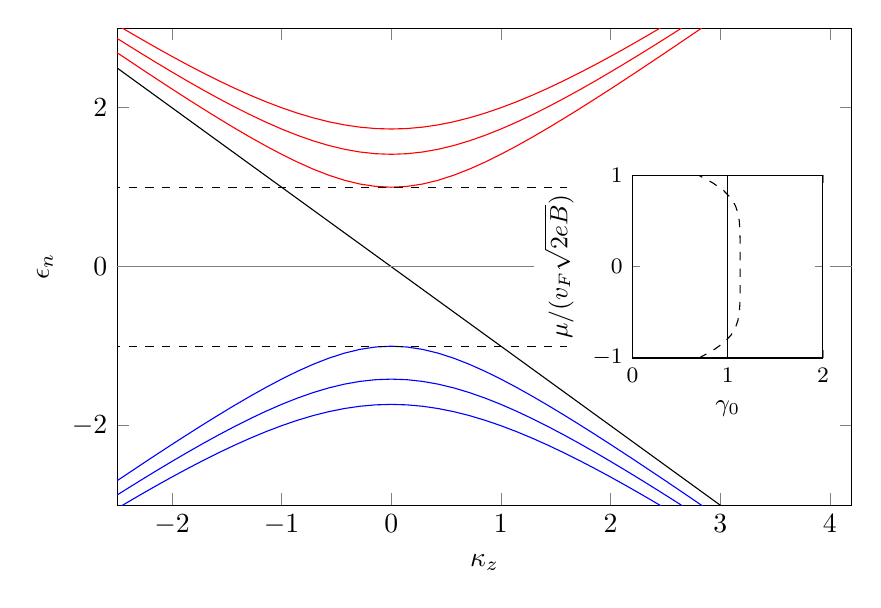
\begin{tikzpicture}
  \begin{axis}[
    width=0.9\textwidth,
    height=0.63\textwidth,
    domain=-3:4,
    xmin=-2.5,xmax=4.2,
    ymin=-3, ymax=3,
    samples=50,
    xlabel=\( \kappa_z \),
    ylabel=\( \epsilon_n \),
    ]
    \addplot[mark=none, samples=2] {-x};
    \foreach \n in {1,2,3}{
      \addplot[mark=none, red] {sqrt(\n + x^2)};
      \addplot[mark=none, blue] {-sqrt(\n + x^2)};
    }

    \addplot[dashed, domain=-3:1.6] {1};
    \addplot[dashed, domain=-3:1.6] {-1};
    \addplot[thin, gray, domain=-3:5] {0};
    \fill[white] (axis cs:1.3,-0.8) rectangle (axis cs:4,0.8); %% Pad label of inset
    \coordinate (insetPos) at (axis cs: 2.2,0);
  \end{axis}
  \begin{axis}[at={(insetPos)}, anchor=west, footnotesize, height=3.9cm, width=4cm,
    axis background/.style={fill=white},
    xlabel=\( \gamma_0 \),
    ylabel=\( \mu / (v_F \sqrt{2e B} ) \),
    xtick={0,1,2},
    ytick={-1,0,1},
    ymin=-1,ymax=1,
    xmin=0, xmax=2,
    ]
    \draw (axis cs:1,-1) -- (axis cs:1,1);
    \addplot[domain=-1:1, dashed] ({exp(-(x / 1.1)^6) + 0.13}, x);
  \end{axis}
\end{tikzpicture}

  \caption{The Landau level of an untilted Weyl cone.
    The inset shows the prefactor \( \gamma_0 \) of the response function for a small finite potential \( \mu \), within the energy interval indicated with dashed lines.
    In the inset, the solid line is computed at zero temperature, while the dashed line is computed at a small finite temperature.
    Figure inspired by \textcite{arjonaFingerprintsConformalAnomaly2019}.
    }
    \label{fig:platau}
\end{figure}


\section{Discussion of results}
In the static and local limit $\lim_{\omega \to 0} \lim_{\vec{q}\to 0}$ the  transverse response function $\chi^{xy}$ of the charge current to a temperature perturbation
\begin{equation}
  J^x = \chi ^{xy} \frac{- \nabla^y T}{T}
\end{equation}
from a single Dirac point was found  to be
\begin{equation}
  \lim_{\omega \to 0} \lim_{\vec{q}\to 0}
  \chi ^{xy}
  =
  \gamma_{N}
  \frac{e^2 B v_F}{4 (2\pi )^2 \hbar },
\end{equation}
with $\gamma _N$ a prefactor dependent on how many landau levels are included in the final evaluation of the response function.
The response function is independent of the chirality $s$ of the Dirac point.
It was found that $\gamma _0 = 1, \gamma _{20} \approx 2$ and that the prefactor goes like $\log N$.

Firstly, the result differ slightly from that found by~\textcite{arjonaFingerprintsConformalAnomaly2019}
\begin{equation}
  \lim_{\omega \to 0} \lim_{\vec{q}\to 0}
  \chi ^{xy}
  =
  2 \gamma_{N}
  \frac{e^2 B v_F}{4 (2\pi )^2 \hbar },
\end{equation}
which differ by a factor of two.

Secondly, the sum will diverge as $N\to \infty $.
However, not all Landau levels are filled, and thus the sum should not be taken to all levels.
Similarly to a Quantum Hall effect, the number of filled bands, the filling factor $\nu $, is inverse proportional to the $B$-field strength
\begin{equation}
  \nu \propto \frac{1}{B}.
\end{equation}
Thus, we expect that the $N$-sum should be truncated at a Landau level, given by the filling factor $\nu $.
A detailed derivation of the exact truncation of the $N$-sum has not been done.
If a precise result for the numerical prefactor is found to be of importance, this should be straightforward.

The divergence is not discussed by~\citeauthor{arjonaFingerprintsConformalAnomaly2019}, where only the values of $N = 0$ and  $N=20$ are given, and the final result is that of $N=20$.
Furthermore, they state that the contributions from higher values of $N$ decrease very rapidly.
However, we found the contributions to go like $1 /x$, which is not decreasing rapidly enough to give a finite total contribution, thus giving the total contribution diverging logarithmically.
\todo{Say that we are communicating with them  to better understand their choice of truncation?}
Comparing our result with the different procedure done by~\citeauthor{chernodubGenerationNernstCurrent2018}~\cite{chernodubGenerationNernstCurrent2018}, the numerical prefactor found in our calculation including only the first term ($M=0$) coincides very well with the numerical prefactor found there, with a ratio of $16 / 18$.

\backmatter
\appendix
\chapter{Contributions from symmetric energy-momentum tensor}
As noted in the main text, there are some subtlety in the definition of the energy-momentum tensor.
The \emph{canonical} definition, which we have used in the main text, is in general not symmetric.
The tensor enter our calculation from the conservation law
\[
\partial_\mu T^{\mu \nu} = 0,
\]
which for \( \nu = 0 \) is nothing more than the conservation law of energy: \( \partial_t \epsilon - \vec{\nabla} \vec{J}_\epsilon = 0 \), where \( \epsilon \) is energy density and \( \vec{J}_\epsilon \) is the energy current.
In the calculation by \citeauthor{arjonaFingerprintsConformalAnomaly2019}\cite{arjonaFingerprintsConformalAnomaly2019}, the symmetrized energy-momentum tensor
\[
T_S^{\mu \nu} = \frac{T^{\mu \nu} + T^{\nu \mu}}{2}
\]
was used.
In this appendix we show the contributions of the symmetric tensor.
The contributions from \( T^{\mu \nu} \) and \( T^{\nu \mu} \) is shown to be equal in the non-tilted case.

\section{No tilt}
In the main text we have already found the contributions from the canonical tensor, and so we focus here on the contributions from \( T_F^{\mu \nu } = T^{\nu \mu} \).
The relevant element is \( T_F^{y 0} = \frac{v_F}{4}\left( \phi^{\dagger} p_y \phi - p_y\phi^{\dagger} \phi \right) \)

Consider now the latter part of the stress-energy tensor, which is split into two parts
\begin{align}
  \label{eq:113}
  T ^{0y\; (2)} _{\vec{k}+\qvec{q}ns, \vec{k}ms} (\vec{q}) &= +
                                                            \frac{1}{4}
                                                            \int \mathrm{d}y
                                                            e^{iq_y y} v_F
                                                            \phi ^{*}_{\vec{k}+\qvec{q} ns}(y)
                                                            p_y \phi _{\vec{k}ms} (y),\\
  \label{eq:114}
  T ^{0y\; (3)} _{\vec{k}+\qvec{q}ns, \vec{k}ms} (\vec{q}) &= -
                                                            \frac{1}{4}
                                                            \int \mathrm{d}y
                                                            e^{iq_y y} v_F
                                                            \left( p_y\phi ^{*}_{\vec{k}+\qvec{q} ns}(y) \right)
                                                            \phi _{\vec{k}ms}(y).
\end{align}
Recall that $\phi_{\vec{k}ms} (y)$, defined in Eq. (\ref{eq:15}), consists of two $y$-dependent factors:
\(
  \exp \left[-\frac{(y-k_x l_B^2)^2}{2 l_{B}^2 } \right]
\)
and the Hermite polynomials.
The operator $p_y$ thus produces two terms when operating on $\phi $.
The first term, coming from the exponent, is proportional to $y-k_xl_B^2$.
The operator in Eqs. (\ref{eq:113}) and (\ref{eq:114}) acts on $\phi $ with the quantum  number $\vec{k}$ and $\vec{k} + \qvec{q}$, respectively;
when summing the two contributions, everything thus cancels except for a term proportional to $q_x$, which vanishes in the local limit.

It remains to consider the result of $p_y$ operating on the Hermite polynomials.
Let $\tilde{p}_y$ indicate the $p_y$ operator acting only on the Hermite polynomial part of $\phi $, and use the property of Hermite polynomials $\partial _x H_n(x) = 2 n H_{n-1}(x)$~\cite[Eq.~18.9.25]{NIST:DLMF}.
\begin{multline}
      \phi ^{*}_{\vec{k}+\qvec{q}ns}(y) \tilde{p}_y \phi _{\vec{k}ms} =
    -i \hbar \exp \left\{
      - \frac{(y-k_xl_B^2)^2 + (y-(k_x + q_x) l_B^2)^2}{2 l_B^2}
    \right\}\\
    \frac{2}{l_B}\Bigg\{
      (M-1) a _{\vec{k} ms}a _{\vec{k}+\qvec{q} ns} H_{M-2}\left( \frac{y-k_x l_B^2}{l_B} \right) H_{N-1} \left( \frac{y - (k_x+q_x)l_B^2}{l_B} \right)\\
      + M b _{\vec{k} ms} b _{\vec{k}+\qvec{q} ns} H_{M-1} \left( \frac{y - k_xl_B^2}{l_B} \right) H_N \left( \frac{y - (k_x+q_x)l_B^2}{l_B} \right)
    \Bigg\}.
\end{multline}
Completing the square, we get
\begin{multline}
  \int \mathrm{d}y e^{iq_y y} \phi ^{*}_{\vec{k}+\qvec{q} ns}(y) \tilde{p}_y \phi _{\vec{k} ms}(y) =
  -i\hbar
  \exp \left[ -\frac{l_B^2}{4} \left\{ \qvec{q}_y^2 - 2iq_y ( 2k_x + q_x) \right\} \right]\\
  \int \mathrm{d}y
  \exp \left[
    - \left\{
      y + \frac{l_B^2}{2} \left( -iq_y - 2k_x - q_x \right)
    \right\} ^2
    / l_B^2
  \right]\\
  \frac{2}{l_B}\Bigg\{
  (M-1) a _{\vec{k}ms}a _{\vec{k}+\qvec{q} ns} H_{M-2}\left( \frac{y-k_x l_B^2}{l_B} \right) H_{N-1} \left( \frac{y - (k_x+q_x)l_B^2}{l_B} \right)\\
  + M b _{\vec{k} ms} b _{\vec{k}+\qvec{q} ns} H_{M-1} \left( \frac{y - k_xl_B^2}{l_B} \right) H_N \left( \frac{y - (k_x+q_x)l_B^2}{l_B} \right)
  \Bigg\}.
\end{multline}
Upon introducing $\tilde{y} = \frac{y}{l_B} + l_B( -iq_y - q_x - 2k_x) / 2$, as was also done in the main text, the expression reduces to
\begin{multline}
  \int \mathrm{d}y e^{iq_y y} \phi ^{*}_{\vec{k}+\qvec{q} ns}(y) \tilde{p}_y \phi _{\vec{k} ms}(y) =
  -i\hbar
  \exp \left[ -\frac{l_B^2}{4} \left\{ q_x^2 + q_y^2 - 2iq_y ( 2k_x + q_x) \right\} \right]\\
  \int \mathrm{d}\tilde{y} l_B
  \exp \left[
    - \tilde{y}^2
  \right]\\
  \frac{2}{l_B}\Bigg\{
  (M-1) a _{\vec{k}ms}a _{\vec{k}+\qvec{q} ns}
  H_{M-2}\left( \tilde{y} + \frac{l_B}{2}(iq_y + q_x) \right)
  H_{N-1} \left( \tilde{y} + \frac{l_B}{2}(iq_y - q_x) \right)\\
  + M b _{\vec{k} ms} b _{\vec{k}+\qvec{q} ns}
  H_{M-1} \left( \tilde{y} + \frac{l_B}{2}(iq_y + q_x)\right)
  H_N \left( \tilde{y} + \frac{l_B}{2}(iq_y - q_x) \right)
  \Bigg\}.
\end{multline}

Considering now the local limit \( \vec{q} \to 0 \), the expression greatly simplifies, and we may use the orthogonality relation for the Hermite polynomials Eq. \eqref{eq:hermite-ortho}
\[
  \int\limits_{-\infty}^{\infty} \mathrm{d}x e^{-x^2} H_n(x)H_m(x) = \sqrt{\pi} 2^{n} n! \delta_{n,m}
\]
to evaulate the integral.
\begin{equation}
  \label{eq:115}
  \lim_{\vec{q} \to 0} \int \mathrm{d}y e^{iq_y y} \phi ^{*}_{\vec{k}+\qvec{q} ns}(y) \tilde{p}_y \phi _{\vec{k} ms}(y) =
  -i \hbar \sqrt{2}
  \frac{
    \alpha_{k m s} \alpha_{k n s} \sqrt{M-1}
    +
    \sqrt{M}
  }{
    {l_{B} \sqrt{\alpha_{k m s}^2 + 1}\sqrt{\alpha_{k n s} ^2 + 1}}
  }
  \delta_{N, M-1}.
\end{equation}

Similarly, for $T^{0y\; (3)}_{\vec{k}+\qvec{q}ns, \vec{k}ms} (\vec{q})$, one has
\begin{multline}
  \left( \tilde{p}_y \phi ^{*}_{\vec{k}+\qvec{q} ns}(y) \right)
  \phi _{\vec{k} m s}(y) =
  -i \hbar \exp \left\{
    - \frac{(y-k_xl_B^2)^2 + (y-(k_x + q_x) l_B^2)^2}{2 l_B^2}
  \right\}\\
  \frac{2}{l_{B}} \left\{
    (N-1) a_{\vec{k} m s} a_{\vec{k} + \qvec{q} n s} H_{M-1} \left( \frac{y-k_xl_B^2}{l_B} \right)H_{N-2} \left( \frac{y - (k_x + q_x) l_B^2}{l_B} \right) \right.\\
  \left. +
    N b_{\vec{k} m s} b_{\vec{k}+\qvec{q} n s} H_M \left( \frac{y - k_xl_B^2}{l_B} \right) H_{N-1}\left( \frac{y-(k_x+q_x) l_B^2}{l_B} \right)
  \right\}
\end{multline}
which with the same procedure as above gives
\begin{equation}
 \lim_{\vec{q}\to 0} \int \mathrm{d}y e^{iq_y y}
  \left( \tilde{p}_y \phi ^{*}_{\vec{k}+\qvec{q} ns}(y) \right)
  \phi _{\vec{k} m s}(y)
  =
  -i \hbar \sqrt{2}
  \frac{
    \alpha_{k m s} \alpha_{k n s} \sqrt{N-1}
    +
    \sqrt{N}
  }{
    {l_{B} \sqrt{\alpha_{k m s}^2 + 1}\sqrt{\alpha_{k n s} ^2 + 1}}
  }
  \delta_{M, N-1}.
\end{equation}

\section{With tilt}
In the tilted case, we have shown in the main text that \todo{insert ref}
\[
  T^{\mu 0} = \frac{i}{2}
  \left[\partial_i \bar{\psi} \Gamma^j \gamma^0 \Gamma^{\mu} \psi
    - \bar{\psi} \Gamma^{\mu} \gamma^0 \Gamma^j \partial_j \psi
  \right].
\]
Swapping the indices, we have for \( \mu \neq 0 \) \cite{vanderwurffMagnetovorticalThermoelectricTransport2019}
\[
  T^{0 i} = \frac{i}{2} [\bar{\psi} \gamma^0 \partial^{\mu } \psi
  - \partial^{\mu }\bar{\psi} \gamma^{0 } \psi ].
\]
In our work, we have considered only tilt perpendiculat to the thermal gradient,  so the component of the energy-momentum tensor of interest are not affected by the tilt.

or
\begin{align}
  T_{\vec{k} + \qvec{q} ns, \vec{k} ms}^{0y (2)} (\vec{q}) &=
                                                             + \frac{1}{4} \int \mathrm{d} y
                                                             e^{iq_{y} y} v_{F}
                                                             \phi ^{*}_{\vec{k}+\qvec{q} ns} (y) p_{y} \phi _{\vec{k} m s} (y),\\
  T_{\vec{k} + \qvec{q} ns, \vec{k} ms}^{0y (3)} (\vec{q}) &=
                                                             - \frac{1}{4} \int \mathrm{d} y
                                                             e^{iq_{y} y} v_{F}
                                                             (p_{y} \phi ^{*}_{\vec{k}+\qvec{q} ns} (y))  \phi _{\vec{k} m s} (y).
\end{align}
Firstly, we note that
\[
  [p_{y} , e^{\theta /2 \sigma _{x}}] = 0.
\]
Furthermore, exactly as for the untilted case, the momentum operator acting on the exponential prefactor of \(\phi \) gives contributions proportional to \(q_{x}\).
In the local limit \(q\to  0\) this term vanishes, and we need only consider the effect of the momentum operator acting on the Hermite polynomials.

Denote by \(\tilde{p}_{y}\) the momentum operator \(p_{y}\) acting only on the Hermite polynomial part of \(\phi \).
Furthermore, we will use the property of Hermite polynomials \(\partial _{x} H_{n} (x) = 2 n H_{n-1} (x)\) \cite[Eq.~18.9.25]{NIST:DLMF}.
\begin{align}
  \tilde{p}_{y} \phi _{\vec{k} ms} &=
  -i \hbar
  e^{\theta /2 \sigma _{x}}
  e^{-\frac{1}{2} \chi ^2}
  \partial _{y}
  \begin{pmatrix}
    a_{\vec{k} m s} H_{M-1} (\chi) \\
    b_{\vec{k} ms} H_{M} (\chi)
  \end{pmatrix}\\
                                   &=
                                     -i \hbar
                                     e^{\theta /2 \sigma _{x}}
                                     e^{-\frac{1}{2} \chi ^2}
                                     2 \frac{\partial \chi }{\partial y}
                                     \begin{pmatrix}
                                       a_{\vec{k} m s} (M-1) H_{M-2} (\chi) \\
                                       b_{\vec{k} ms} (M) H_{M-1} (\chi)
                                     \end{pmatrix}\\
                                   &=
                                     -i \hbar
                                     e^{\theta /2 \sigma _{x}}
                                     e^{-\frac{1}{2} \chi ^2}
                                     \frac{2 \sqrt{\alpha}}{ l_{B} }
                                     \begin{pmatrix}
                                       a_{\vec{k} m s} (M-1) H_{M-2} (\chi) \\
                                       b_{\vec{k} ms} (M) H_{M-1} (\chi)
                                     \end{pmatrix}.
\end{align}
And thus, recalling that
\[
  e^{\theta \sigma _{x}} =
  \begin{pmatrix}
    1 & -t_{x}\\
    -t_{x} & 1
  \end{pmatrix}
  \frac{1}{\sqrt{1-t_{x}^2}},
\]
we find the product
\begin{multline}
  \phi ^{*} _{\vec{k} + \qvec{q} ns} (y) \tilde{p}_{y} \phi _{\vec{k} m s}
  % = -\frac{i\hbar 2 \sqrt{\alpha } }{ l_{B} }
  % e^{-\frac{1}{2} \chi _{\vec{k}}^2 - \frac{1}{2} \chi _{\vec{k} + \qvec{q}} ^2}
  % \phi ^{*}_{\vec{k} + \qvec{q} ns}(y)
  % e^{\theta \sigma _{x}}
  % \phi _{\vec{k} ms} (y)\\
  % %
  = -\frac{i\hbar 2 \sqrt{\alpha } }{l_{B} \sqrt{1 - t_{x}^2} }
  e^{-\frac{1}{2} \chi _{\vec{k}}^2 - \frac{1}{2} \chi _{\vec{k} + \qvec{q}} ^2}\\
  \Big[
  a_{\vec{k} + \qvec{q} ns} H_{N-1}(\chi_{\vec{k}+\qvec{q}})
  \left\{a_{\vec{k} ms} (M-1) H_{M-2} (\chi_{\vec{k}}) - t_{x} b_{\vec{k} ms} M H_{M-1} (\chi_{\vec{k}})\right\}\\
  +
  b_{\vec{k} + \qvec{q} ns} H_{N} (\chi_{\vec{k} + \qvec{q}})
  \left\{-t_{x} a_{\vec{k} ms} (M-1) H_{M-2} (\chi_{\vec{k}}) + b_{\vec{k} ms} M H_{M-1} (\chi_{\vec{k}})\right\}
  \Big].
\end{multline}
Completing the square and substituting
\[
  \tilde{y} = \frac{\sqrt{ \alpha  }}{l_{B}}
  \left(y - \frac{l_{B}^2}{2 \alpha } (i q_{y} + (2 k'_x + q' _x) ) \right)
\]
gives
\begin{multline}
  \int \mathrm{d}y
  e^{i q_{y}}
  \phi ^{*}_{\vec{k} + \qvec{q} ns}(y) \tilde{p}_{y}
  \phi_{\vec{k} ms} (y)
  =
  - \frac{i\hbar 2 \sqrt{\alpha} }{l_{B} \sqrt{1 - t_{x}^2} }
  \exp
  \left[
    - \frac{l_{B}^2}{4 \alpha } (q_{y}^2 - 2 i (2k' _x + q' _x) q_{y} + (q' _x)^2 )
  \right  ]\\
  \int \mathrm{d} \tilde{y} \frac{l_{B}}{\sqrt{\alpha } }\\
  \Big[
  a_{\vec{k} + \qvec{q} ns} H_{N-1}( \chi _{\vec{k} + \qvec{q}} )
  \left\{
    a_{\vec{k} ms} (M-1) H_{M-2} ( \chi _{\vec{k}} )
    - t_{x} b_{\vec{k} ms} M H_{M-1} ( \chi _{\vec{k}} ) \right\}\\
  +
  b_{\vec{k} + \qvec{q} ns} H_{N} ( \chi _{\vec{k} + \qvec{q}} )
  \left\{
    -t_{x} a_{\vec{k} ms} (M-1) H_{M-2} ( \chi _{\vec{k}} )
    + b_{\vec{k} ms} M H_{M-1} ( \chi _{\vec{k}} )
  \right\}
  \Big].
\end{multline}

We must now evaluate the integral, and express the result in the \( \Xi \)-functions.
\[
    \begin{pmatrix}
      a_{\vec{k} + \qvec{q} n s} H_{N-1} ( \chi _{\vec{k} + \qvec{q}} )\\
      b_{\vec{k} + \qvec{q} ns} H_N ( \chi _{\vec{k} + \qvec{q}} )
    \end{pmatrix}^{T}
  \underbrace{
    \begin{pmatrix}
      1 & -t_x\\
      -t_x & 1
    \end{pmatrix}
    }_{T}
    \begin{pmatrix}
      a_{\vec{k} m s} (M-1) H_{M-2} (\chi_{\vec{k}})\\
      b_{\vec{k} m s} M H_{M-1} ( \chi _{\vec{k}} )
    \end{pmatrix}
\]
For each of the entries in \( T \), we get a product on of Hermite polynomials.
Where the untilted cone had two such terms, the tilt parameter \( t _x \) now gives two extra products, which we must evaluate.
Let \( M^{(2)}_{ij} \) be the product corresponding to \( T_{ij} \), i.e.
\begin{align}
  M^{(2)}_{11} &= \phantom{-t_x} a_{\vec{k} + \qvec{q} ns} a_{\vec{k} ms} (M-1) H_{N-1} (\chi_{\vec{k} + \qvec{q}}) H_{M-2} (\chi_{\vec{k}}),\\
  M^{(2)}_{12} &= -t_x a_{\vec{k} + \qvec{q} ns} b_{\vec{k} ms} M H_{N-1} (\chi_{\vec{k} + \qvec{q}}) H_{M-1} (\chi_{\vec{k}}),\\
  M^{(2)}_{21} &= -t_x b_{\vec{k} + \qvec{q} ns} a_{\vec{k} ms} ( M-1 ) H_{N} (\chi_{\vec{k} + \qvec{q}}) H_{M-2} (\chi_{\vec{k}}),\\
  M^{(2)}_{22} &= \phantom{-t_x} b_{\vec{k} + \qvec{q} ns} b_{\vec{k} ms} M H_N (\chi_{\vec{k} + \qvec{q}}) H_{M-1} (\chi_{\vec{k}}).
\end{align}
We want to evaluate
\begin{equation}
  \label{eq:116}
  F^{(2)}_{ij} =
  \left[(\alpha_{\vec{k} m s}^2 + 1) ( \alpha _{\vec{k} + \qvec{q} n s}^2 + 1 )\right]^{\frac{1}{2}}
  \int \mathrm{d} \tilde{y}
  e^{-\tilde{y}^2}
  M^{(2)}_{ij},
\end{equation}
with the prefactor introduced for later convenience.

Notice that
\todo{Verify \( l_B \) in this section}
\begin{equation}
  F^{(2)}_{12}
  = -t_x \sqrt{\alpha}  \sqrt{\frac{M}{2}} \alpha _{k+q, n} \Xi_2(\bar{\vec{q}}, m\mp 1, n).
\end{equation}
and
\begin{equation}
  \label{eq:117}
  F^{(2)}_{21}
  =
  -t_{x} \sqrt{\alpha} \sqrt{\frac{M-1}{2}} \frac{a_{\vec{k} m s}^2}{l_B a_{\vec{k} m \mp 1 s}}
  \Xi_{1} (\bar{\vec{q}}, m \mp 1, n, s).
\end{equation}
\( F^{(2)}_{11} \) and \( F^{(2)}_{22} \) are the same as for the untilted case:
\begin{equation}
  \label{eq:118}
  F^{(2)}_{11} = \sqrt{\alpha}  \frac{\alpha_{\vec{k} m s} \alpha_{\vec{k} + \qvec{q} ns} \sqrt{M-1} }{ l_B \sqrt{2} }
  \Xi_{1} (\bar{\vec{q}}, m\mp 1, n\mp 1, s),
\end{equation}
and
\begin{equation}
  \label{eq:119}
  F^{(2)}_{22} =
  \sqrt{\alpha }
  \frac{\sqrt{M} }{l_B \sqrt{2} }
  \Xi_{1} ( \bar{\vec{q}}, m, n, s ).
\end{equation}
In summary we have
\begin{align}
  \label{eq:120}
  T^{0y~(2)}_{\vec{k} + \qvec{q} ns, \vec{k} ms} (\vec{q}) &= + \frac{v_F}{4} \int \mathrm{d} y
  e^{i q_y q} \phi _{\vec{k} + \qvec{q} ns}^{*} (y) p_{y} \phi _{\vec{k} ms} (y)\\
&= -\frac{ i \hbar v_{F} }{2}
                                                                                     \Gamma _{\vec{k} \qvec{q} m n s}^+
\sum\limits_{i,j}^{} F^{(2)}_{ij},
\end{align}
where
\[
  \Gamma _{\vec{k} \qvec{q} m n s}^+ =
  \frac{
  \exp
  \left[
    - \frac{l_{B}^2}{4 \alpha } (q_{y}^2 - 2 i (2k' _x + q' _x) q_{y} + (q' _x)^2 )
  \right  ]
}{
  \left[(\alpha_{\vec{k} m s}^2 +1) (\alpha_{\vec{k} + \qvec{q} ns} ^2 + 1)\right]^{\frac{1}{2}}
  \sqrt{1 - t_x^2 }}
\]

In a similar procedure, we find \( T^{0y~(2)}_{\vec{k}+\qvec{q} ns, \vec{k} ms}(\vec{q}) \).
\begin{equation}
  \tilde{p}_y \phi^{*}_{\vec{k}+\qvec{q} m s} = \frac{-i \hbar \sqrt{\alpha } }{l_{B}}  e^{-\frac{1}{2} \chi ^2}
                                   \begin{pmatrix}
                                     a_{\vec{k}+\qvec{q} m s} (M-1) H_{M-2} (\chi) \\
                                     b_{\vec{k}+\qvec{q} m s} (M) H_{M-1} (\chi)
                                   \end{pmatrix}.
\end{equation}
And thus,
\begin{multline}
  \left( \tilde{p}_y \phi ^{*} _{\vec{k} + \qvec{q} ns} (y) \right) \phi _{\vec{k} m s}
  = -\frac{i\hbar 2 \sqrt{\alpha } }{l_{B} \sqrt{1 - t_{x}^2} }
  e^{-\frac{1}{2} \chi _{\vec{k}}^2 - \frac{1}{2} \chi _{\vec{k} + \qvec{q}} ^2}\\
  \Big[
  a_{\vec{k} + \qvec{q} ns} (N-1) H_{N-2}(\chi_{\vec{k}+\qvec{q}})
  \left\{a_{\vec{k} ms} H_{M-1} (\chi_{\vec{k}}) - t_{x} b_{\vec{k} ms} H_{M} (\chi_{\vec{k}})\right\}\\
  +
  b_{\vec{k} + \qvec{q} ns} N H_{N-1} (\chi_{\vec{k} + \qvec{q}})
  \left\{-t_{x} a_{\vec{k} ms}  H_{M-1} (\chi_{\vec{k}}) + b_{\vec{k} ms} H_{M} (\chi_{\vec{k}})\right\}
  \Big].
\end{multline}
With the now well-known completion of the square and substitution, we have
\begin{multline}
  \int \mathrm{d}y
  e^{i q_{y}}
  \left[\tilde{p}_y \phi ^{*}_{\vec{k} + \qvec{q} ns}(y) \right]
  \phi_{\vec{k} ms} (y)
  =
  - \frac{i\hbar 2 \sqrt{\alpha} }{l_{B} \sqrt{1 - t_{x}^2} }
  \exp
  \left[
    - \frac{l_{B}^2}{4 \alpha } (q_{y}^2 - 2 i (2k' _x + q' _x) q_{y} + (q' _x)^2 )
  \right  ]\\
  \int \mathrm{d} \tilde{y} \frac{l_{B}}{\sqrt{\alpha } }\\
  \Big[
  a_{\vec{k} + \qvec{q} ns} (N-1) H_{N-2}(\chi_{\vec{k}+\qvec{q}})
  \left\{a_{\vec{k} ms} H_{M-1} (\chi_{\vec{k}}) - t_{x} b_{\vec{k} ms} H_{M} (\chi_{\vec{k}})\right\}\\
  +
  b_{\vec{k} + \qvec{q} ns} N H_{N-1} (\chi_{\vec{k} + \qvec{q}})
  \left\{-t_{x} a_{\vec{k} ms}  H_{M-1} (\chi_{\vec{k}}) + b_{\vec{k} ms} H_{M} (\chi_{\vec{k}})\right\}
  \Big].
\end{multline}
Denote the terms of the integrand by
\begin{align}
  M^{(3)}_{11} &= \phantom{-t_x} a_{\vec{k} + \qvec{q} ns} a_{\vec{k} ms} (N-1) H_{N-2} (\chi_{\vec{k} + \qvec{q}}) H_{M-1} (\chi_{\vec{k}}),\\
  M^{(3)}_{12} &= -t_x a_{\vec{k} + \qvec{q} ns} b_{\vec{k} ms} (N-1) H_{N-2} (\chi_{\vec{k} + \qvec{q}}) H_{M} (\chi_{\vec{k}}),\\
  M^{(3)}_{21} &= -t_x b_{\vec{k} + \qvec{q} ns} a_{\vec{k} ms} N H_{N-1} (\chi_{\vec{k} + \qvec{q}}) H_{M-1} (\chi_{\vec{k}}),\\
  M^{(3)}_{22} &= \phantom{-t_x} b_{\vec{k} + \qvec{q} ns} b_{\vec{k} ms} N H_{N-1} (\chi_{\vec{k} + \qvec{q}}) H_{M} (\chi_{\vec{k}}).
\end{align}
We must evaluate
\begin{equation}
  \label{eq:121}
  F^{(3)}_{ij} = \left[(\alpha_{\vec{k} m s}^2  + 1) ( \alpha _{\vec{k} + \qvec{q} ns}^2 + 1 )\right]^{\frac{1}{2}} \int \mathrm{d} \tilde{y} e^{-\tilde{y}^2} M^{(3)}_{ij}.
\end{equation}
From the untilted case we know
\begin{align}
  F^{(3)}_{11} &= \sqrt{\frac{N-1}{2}}
                 \frac{\alpha_{\vec{k} m s} \alpha_{\vec{k}+\qvec{q} n s}}{l_{B} \alpha _{\vec{k} + \qvec{q} n \mp 1 s}}
                 \Xi_2( \bar{\vec{q}}, m\mp 1, n\mp 1, s ),\\
  F^{(3)}_{22} &= \sqrt{\frac{N}{2}}
                 \frac{1}{l_{B} \alpha _{\vec{k} + \qvec{q} n s}}
                 \Xi_{2} (\bar{\vec{q}}, m, n, s).
\end{align}
Furthermore,
\begin{align}
  F^{(3)}_{12} &= -t_x \frac{\alpha _{\vec{k} + \qvec{q} n}}{\alpha _{\vec{k}+\qvec{q} n \mp 1} l_{B}}
                 \sqrt{\frac{N-1}{2}}
                 \Xi_{2} (\bar{\vec{q}}, m, n \mp 1, s),\\
  F^{(3)}_{21} &= -\frac{t_x}{l_{B}}
                 \sqrt{\frac{N}{2}}
                 \frac{\alpha_{\vec{k} m}}{\alpha _{\vec{k} + \qvec{q} n}}
                 \Xi_2 ( \bar{\vec{q}}, m \mp 1, n, s ).
\end{align}
We thus have
\begin{align}
  \label{eq:122}
  T^{0y~(3)}_{\vec{k} + \qvec{q} ns, \vec{k} ms} (\vec{q})
  &= - \frac{v_F}{4}
    \int \mathrm{d} y
    e^{i q_y y}
    \left( p_y \phi ^{*}_{\vec{k} + \qvec{q} ns}(y) \right) \phi _{\vec{k} m s}(y)\\
  &= \frac{i \hbar v_F}{2}
    \Gamma ^{+}_{\vec{k} \qvec{q} m n s}
    \sum\limits_{ij}^{} F^{(3)}_{ij}.
\end{align}

\begin{summary}
The non-canonical part of the energy-momentum tensor \( T_F^{\mu \nu} = T^{\nu \mu} \) in a tilted system have the matrix elements
  \begin{align}
    T^{0y~(2)}_{\vec{k} + \qvec{q} ns, \vec{k} ms} (\vec{q})
    &= -\frac{ i \hbar v_{F} }{2}
      \Gamma _{\vec{k} \qvec{q} m n s}^+
      \sum\limits_{i,j}^{} F^{(2)}_{ij},\\
    T^{0y~(3)}_{\vec{k} + \qvec{q} ns, \vec{k} ms} (\vec{q})
    &= \frac{i \hbar v_F}{2}
      \Gamma ^{+}_{\vec{k} \qvec{q} m n s}
      \sum\limits_{ij}^{} F^{(3)}_{ij}.
  \end{align}
  with
  \[
    \Gamma _{\vec{k} \qvec{q} m n s}^{\pm} =
    \frac{
      \exp
      \left[
        - \frac{l_{B}^2}{4 \alpha } (q_{y}^2 + (q' _x)^2) \pm  i q_y l_B^2 (k' _x + \frac{q'_x}{2} )  )
      \right  ]
    }{
      \left[(\alpha_{\vec{k} m s}^2 +1) (\alpha_{\vec{k} + \qvec{q} ns} ^2 + 1)\right]^{\frac{1}{2}}
    }
  \]
  and where the factors \( F_{ij}^{(n)} \) where found to be
  \begin{align}
    F^{(2)}_{12}
    &= -t_x \sqrt{\alpha}  \sqrt{\frac{M}{2}} \alpha _{k+q, n} \Xi_2(\bar{\vec{q}}, m\mp 1, n),\\
    F^{(2)}_{21}
    &=
      -t_{x} \sqrt{\alpha} \sqrt{\frac{M-1}{2}} \frac{a_{\vec{k} m s}^2}{l_B a_{\vec{k} m \mp 1 s}}
      \Xi_{1} (\bar{\vec{q}}, m \mp 1, n, s),\\
    F^{(2)}_{11} &= \sqrt{\alpha}  \frac{\alpha_{\vec{k} m s} \alpha_{\vec{k} + \qvec{q} ns} \sqrt{M-1} }{ l_B \sqrt{2} }
                   \Xi_{1} (\bar{\vec{q}}, m\mp 1, n\mp 1, s),\\
    F^{(2)}_{22} &=
                   \sqrt{\alpha }
                   \frac{\sqrt{M} }{l_B \sqrt{2} }
                   \Xi_{1} ( \bar{\vec{q}}, m, n, s ),\\
    F^{(3)}_{11} &= \sqrt{\frac{N-1}{2}}
                   \frac{\alpha_{\vec{k} m s} \alpha_{\vec{k}+\qvec{q} n s}}{l_{B} \alpha _{\vec{k} + \qvec{q} n \mp 1 s}}
                   \Xi_2( \bar{\vec{q}}, m\mp 1, n\mp 1, s ),\\
    F^{(3)}_{22} &= \sqrt{\frac{N}{2}}
                   \frac{1}{l_{B} \alpha _{\vec{k} + \qvec{q} n s}}
                   \Xi_{2} (\bar{\vec{q}}, m, n, s),\\
    F^{(3)}_{12} &= -t_x \frac{\alpha _{\vec{k} + \qvec{q} n}}{\alpha _{\vec{k}+\qvec{q} n \mp 1} l_{B}}
                   \sqrt{\frac{N-1}{2}}
                   \Xi_{2} (\bar{\vec{q}}, m, n \mp 1, s),\\
    F^{(3)}_{21} &= -\frac{t_x}{l_{B}}
                   \sqrt{\frac{N}{2}}
                 \frac{\alpha_{\vec{k} m}}{\alpha _{\vec{k} + \qvec{q} n}}
                 \Xi_2 ( \bar{\vec{q}}, m \mp 1, n, s ).
\end{align}
\end{summary}

\chapter{Conformal symmetry of a tilted system}
The origin of the term \emph{conformal anomaly} is the \emph{conformal symmetry}.
Under the conformal transformation, the massless \gls{qed} Lagrangian is invariant, as shown in the main text.
Specifically, the \gls{qed} Lagrangian
\[
\mathcal{L} = - \frac{1}{4} F^{\mu \nu }F_{\mu \nu} + i \bar{\psi} \slashed{D} \psi,
\]
with the usual \( \bar{\psi} = \psi^{\dagger} \gamma^0, \slashed{D} = \gamma^{\mu} D_{\mu}, D_{\mu} = \partial_{\mu - i e A_{\mu}} \) transforms under the scaling
\[
x \to \lambda^{-1}, \: A_{\mu} \to \lambda A_{\mu}, \: \psi \to \lambda^{\frac{3}{2}} \psi,
\]
as
\[
\mathcal{L} \to \lambda^4 \mathcal{L}.
\]
The action \( S = \int \mathrm{d}^4x \mathcal{L} \) is thus invariant (as \( \mathrm{d}^4x \to \lambda^{-4}\mathrm{d}^4x \)), and the theory is classically manifestly scale invariant.

Consider now the tilted Dirac Lagrangian considered in our work,
\begin{equation}
  \label{eq:154}
  \mathcal{L} k i\bar{\psi} \Gamma^{\mu} \partial_{\mu} \psi,
\end{equation}
with \( \Gamma^{\mu} = \gamma^{\mu} + t^{\mu} \gamma_P \gamma^0 \), where \( \gamma_P = I_4 \) when inversion summery is broken and \( \gamma_P = \gamma^5 \) for inversion symmetric systems.
The tilt parameter \( t^{\mu} = (0, \vec{t}) \) is invariant under scaling, and thus also this theory is classically scale invariant.


\printglossaries

\printbibliography

% \includepdf{endpagethesis.pdf}
\end{document}
